\documentclass[12pt]{report}

\usepackage[utf8]{inputenc}
\usepackage[T1]{fontenc}
\usepackage[english]{babel}
\usepackage[a4paper, top=2.54cm, bottom=2.54cm, left=3.17cm, right=2.54cm]{geometry}
\usepackage{mathptmx}
\usepackage{setspace}
\usepackage{titlesec}
\usepackage{tocloft}
\usepackage{graphicx}
\usepackage{amsmath}
\usepackage{fancyhdr}
\usepackage{indentfirst}
\usepackage{xcolor}
\usepackage{caption}
\usepackage{enumitem}
\usepackage{hyperref}
\usepackage{booktabs}
\usepackage{float}
\usepackage{cite}
\usepackage[ruled,vlined,linesnumbered]{algorithm2e}
\hypersetup{colorlinks=true, linkcolor=black, citecolor=black, urlcolor=blue}

\setlength{\headheight}{15pt}
\doublespacing
\setlength{\parindent}{1.27cm}
\setlength{\parskip}{0pt}
\setcounter{secnumdepth}{3}
\renewcommand{\thetable}{\Roman{table}}

% Header/Footer
\pagestyle{fancy}
\fancyhf{}
\fancyfoot[C]{\thepage}
\renewcommand{\headrulewidth}{0pt}

% Chapter format
\titleformat{\chapter}[block]
  {\normalfont\normalsize\bfseries\centering}
  {}
  {0pt}
  {}
\titlespacing*{\chapter}{0pt}{-20pt}{12pt}

% Make section numbering independent of chapter (like article class)
\renewcommand{\thesection}{\arabic{section}}
\renewcommand{\thesubsection}{\thesection.\arabic{subsection}}
\renewcommand{\thesubsubsection}{\thesubsection.\arabic{subsubsection}}

\titleformat{\section}{\normalfont\normalsize\bfseries}{\thesection}{1em}{}
\titleformat{\subsection}{\normalfont\normalsize\bfseries}{\thesubsection}{1em}{}
\titleformat{\subsubsection}{\normalfont\normalsize\bfseries}{\thesubsubsection}{1em}{}

% TOC customization
\renewcommand{\cfttoctitlefont}{\hfil\normalfont\normalsize\bfseries}
\renewcommand{\cftaftertoctitle}{\hfil}
\renewcommand{\cftloftitlefont}{\hfil\normalfont\normalsize\bfseries}
\renewcommand{\cftafterloftitle}{\hfil}
\renewcommand{\cftlottitlefont}{\hfil\normalfont\normalsize\bfseries}
\renewcommand{\cftafterlottitle}{\hfil}

\setlength{\cftbeforetoctitleskip}{0pt}
\setlength{\cftaftertoctitleskip}{6pt}
\setlength{\cftbeforeloftitleskip}{0pt}
\setlength{\cftafterloftitleskip}{6pt}
\setlength{\cftbeforelottitleskip}{0pt}
\setlength{\cftafterlottitleskip}{6pt}

\renewcommand{\cftchapdotsep}{\cftdotsep}
\renewcommand{\cftchapfont}{\normalfont\bfseries}
\renewcommand{\cftchappagefont}{\normalfont\bfseries}

% Force babel not to override \contentsname
\addto\captionsenglish{%
  \renewcommand{\contentsname}{TABLE OF CONTENTS}%
  \renewcommand{\listfigurename}{LIST OF FIGURES}%
  \renewcommand{\listtablename}{LIST OF TABLES}%
}

% Unnumbered chapter with TOC entry
\newcommand{\chapterx}[1]{%
  \chapter*{#1}%
  \addcontentsline{toc}{chapter}{#1}%
}

\begin{document}

%% ===================== FRONT MATTER ========================
\pagenumbering{roman}

%% ---- TITLE PAGE -------------------------------------------
\thispagestyle{empty}
\begin{center}
\vspace*{4.5cm}

{\normalsize\bfseries A Vibrotactile Haptic Vest System for\\
Indoor Navigation Assistance for Blind Users}\\[0.5\baselineskip]
{\normalsize\bfseries by}\\[0.5\baselineskip]
{\normalsize\bfseries Hilal \.{I}lhan \& Taha Berk Ko\c{c}}

\vspace{4\baselineskip}

{\normalsize
Department of Electrical and Electronics Engineering\\
Bo\u{g}azi\c{c}i University
}

\vspace{\baselineskip}
{\normalsize October 2026}

\end{center}

\vspace{\baselineskip}
\noindent Principal Investigator:\\
\hspace*{3cm} Kemal C{\i}l{\i}z

\vspace{0.5\baselineskip}
\noindent Coadvisor:\\
\hspace*{3cm} \c{C}a\u{g}atay Ba\c{s}do\u{g}an

\clearpage

%% ---- ACKNOWLEDGMENTS (p. ii) ------------------------------
\setcounter{page}{2}
\chapterx{ACKNOWLEDGMENTS}
\thispagestyle{fancy}

\noindent We would like to express our sincere gratitude to our principal investigator, Prof. Kemal Cılız, and our co-advisor, Prof. Çağatay Başdoğan, for their invaluable guidance, continuous support, and constructive feedback throughout this project. Their expertise in robotics and haptic systems greatly shaped the direction and quality of this work.

We are also grateful to the members of the Boğaziçi University community who volunteered as participants in our user studies. Their time and feedback were essential to the evaluation and refinement of the proposed haptic signal framework.


\clearpage

%% ---- ABSTRACT (p. iii) ------------------------------------
\chapterx{ABSTRACT}
\thispagestyle{fancy}

\noindent This work presents a vibrotactile haptic vest system designed to assist blind users in navigating indoor environments. Navigating an unfamiliar indoor space requires a person to determine their position, identify a suitable route, and respond to obstacles and changes in direction. The proposed system addresses these tasks by combining environmental perception, performed by a user-mounted ZED 2 stereo camera, with navigation guidance delivered through a wearable vibrotactile vest, so that guidance can be provided without visual displays or continuous spoken instructions.

The haptic interface was developed and evaluated in two phases. In Phase 1, a structured haptic signal library comprising 24 signals across three categories---navigation, warning, and movement modulation---was constructed and evaluated through a user study with 18 participants. Recognition accuracy improved substantially following a brief training session, rising from 43.8\% to 86.0\%, with corresponding improvements in response time and confidence. Warning signals were consistently the most intuitive and reliably recognized category, while navigation signals showed marked improvement after training. Analyses of signal duration and intensity revealed that signal structure and temporal characteristics were the primary drivers of recognition performance, with intensity serving primarily as a modulator of perceived urgency.

In Phase 2, four path-tracking strategies---Non-stop Waypoint, Stop-and-Align, Hybrid, and Non-stop Align Navigation---were designed to translate the user's position and heading relative to a planned route into real-time vibrotactile guidance. The algorithms were validated through two-dimensional and three-dimensional simulation environments, and a ZED 2 stereo camera was integrated for real-time user pose estimation. The remaining work consists of indoor mapping, global and local path planning, closed-loop integration of these components with the vest, and physical navigation experiments, which are described as the continuation of this study.


\clearpage

%% ---- TABLE OF CONTENTS ------------------------------------
\tableofcontents
\clearpage

%% ---- LIST OF FIGURES --------------------------------------
\listoffigures
\addcontentsline{toc}{chapter}{LIST OF FIGURES}
\clearpage

%% ---- LIST OF TABLES ---------------------------------------
\listoftables
\addcontentsline{toc}{chapter}{LIST OF TABLES}
\clearpage

%% ---- LIST OF APPENDICES -----------------------------------
\chapter*{LIST OF APPENDICES}
\addcontentsline{toc}{chapter}{LIST OF APPENDICES}
\thispagestyle{fancy}

\noindent\underline{Appendix}

\vspace{6pt}
\begin{list}{}{%
  \setlength{\leftmargin}{1.5cm}
  \setlength{\labelwidth}{1cm}
  \setlength{\labelsep}{0.5cm}
  \setlength{\itemsep}{6pt}
  \setlength{\parsep}{0pt}
}
\item[A.] Supplementary Materials (Haptic Signal Pattern Visuals, Survey Source Code, Analysis Code)\dotfill
\item[B.] Algorithm Pseudocodes\dotfill
\end{list}

\clearpage

%% ===================== MAIN MATTER =========================
\pagenumbering{arabic}
\setcounter{page}{1}

\addtocontents{toc}{\noindent\textbf{CHAPTER}\par\vspace{-6pt}}

%% ============================================================
%%  CHAPTER 1 — INTRODUCTION
%% ============================================================
\chapter*{\centering CHAPTER 1\\[4pt]INTRODUCTION}
\addcontentsline{toc}{chapter}{1. INTRODUCTION}
\thispagestyle{fancy}

Navigating an unfamiliar indoor environment requires a person to determine their position, identify a suitable route, and respond to obstacles and changes in direction. For blind users, each of these tasks must be accomplished without visual information, which makes independent indoor wayfinding a persistent accessibility challenge. Existing assistive solutions often rely on audio instructions, which can mask environmental sounds that blind users depend on for orientation and safety, or on handheld devices that occupy the hands.

Haptic feedback offers an attractive alternative. It provides intuitive, non-visual, and non-auditory communication, which is particularly valuable in noisy settings or whenever visual and auditory attention must be preserved for primary tasks \cite{Rurenko2025sensing}. By utilizing the tactile channel, additional information can be conveyed without overloading existing sensory modalities \cite{Yan2013adesign}. Prior work has shown that vibrotactile interfaces can guide blind walkers along routes \cite{kammoun2012guiding, flores2015vibrotactile, marston2007nonvisual}, but the combination of a rich, learnable signal vocabulary, an automatically generated route, and a wearable vest remains under-explored.

This project proposes a navigation assistance system for blind users that combines environmental perception with wearable vibrotactile feedback. A ZED 2 stereo camera attached to the user is used for indoor mapping and pose estimation, a navigation module generates a walking path from the map, the destination, and the estimated user pose, and a haptic vest translates the required motion into tactile cues such as turning, moving forward, slowing down, and stopping. The user's subsequent movement is monitored to update the guidance, forming a closed feedback loop between sensing, guidance, and walking.

The project focuses on indoor wayfinding and path following. Its intended contribution is the integration and experimental evaluation of perception, user-relative navigation commands, and an understandable tactile interface in a controlled indoor setting. This document reports the work carried out so far---the design and evaluation of the haptic signal vocabulary and of the path-tracking guidance strategies---and describes how this work will be extended into the complete navigation system.

%% ============================================================
%%  CHAPTER 2 — OBJECTIVES
%% ============================================================
\chapter*{\centering CHAPTER 2\\[4pt]OBJECTIVES}
\addcontentsline{toc}{chapter}{2. OBJECTIVES}
\thispagestyle{fancy}

The main objective of this project is to develop and experimentally evaluate a haptic vest navigation system that assists blind users in reaching a designated indoor destination. To achieve this goal, the system will construct an indoor map from the visual and depth data of the ZED camera, representing both free space and detected obstacles for navigation. The user's position and heading will be estimated within the map coordinate frame to enable continuous localization during movement.

Based on this information, the system will generate a route that maintains appropriate clearance from obstacles and will update the navigation guidance as the user moves through the environment. If time permits, more advanced navigation and path-planning algorithms will also be explored to improve route generation and adaptation to the surrounding environment.

A second objective is to design a compact and learnable vibrotactile signal vocabulary that communicates directional information and navigation states through the haptic vest, and to quantify how well users can recognize and interpret these signals. The mapping, localization, path-planning, and vest-actuation components will then be integrated into a real-time feedback loop.

Finally, the proposed system will be experimentally evaluated under controlled conditions. The evaluation will focus on navigation performance, the users' ability to recognize and interpret vibrotactile cues, perceived workload, and confidence while completing the navigation task.

%% ============================================================
%%  CHAPTER 3 — APPROACH AND METHODOLOGY
%% ============================================================
\setcounter{section}{3}
\setcounter{subsection}{0}
\setcounter{subsubsection}{0}
\chapter*{\centering CHAPTER 3\\[4pt]APPROACH AND METHODOLOGY}
\addcontentsline{toc}{chapter}{3. APPROACH AND METHODOLOGY}
\thispagestyle{fancy}

The proposed setup consists of a human-mounted ZED 2 stereo camera, a compatible processing computer, and a vibrotactile haptic vest (as in Fig.~\ref{fig:Haptic_Vest}) worn by the user. The experimental environment will be a controlled indoor area in which the participant navigates from an initial position to a predefined destination. During navigation, the system uses visual and depth information from the camera to estimate the surrounding environment and the user's motion. Based on this information, navigation instructions are generated and communicated through the vibrotactile vest. The participant is therefore expected to reach the target location primarily by following the haptic guidance, while the camera continuously supplies environmental and localization information.

\begin{figure}[htbp]
    \centering
    \begin{minipage}{0.45\textwidth}
        \centering
        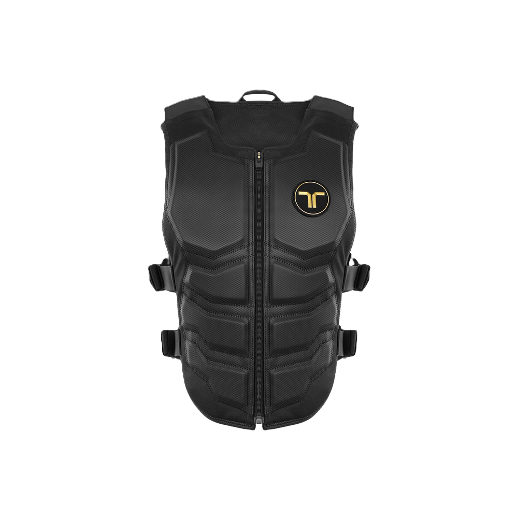
\includegraphics[width=\linewidth]{image2.png}
        \caption{Vibrotactile Haptic Vest \cite{bhaptics}}
        \label{fig:Haptic_Vest}
    \end{minipage}
\end{figure}

The overall system is composed of five cooperating parts: indoor mapping, user position and heading estimation, path planning, haptic signal encoding and sending, and the vest itself. The work reported in this document concentrates on the last two parts---the haptic vocabulary and the encoding of the user's pose relative to a route into vest commands---together with the integration of the ZED 2 camera as the pose source. Mapping and planning are described in the following subsections as the components that complete the pipeline.

\subsection*{Literature Review on Vibrotactile Navigation}

Prior work on vibrotactile navigation provides several design principles that guided the construction of our haptic feedback framework. First, directional information is most naturally conveyed through the spatial location of vibration on the body. This principle, often described as the ``tap-on-the-shoulder'' metaphor, relies on the intuitive association between the stimulated body location and the corresponding external direction \cite{ertan1998wearable, vanveen2004waypoint, vanerp2005waypoint, pielot2008continuous, pielot2010tactilewayfinder, kammoun2012guiding, flores2015vibrotactile, cosgun2014guidance}. Accordingly, navigation and warning signals in our framework are primarily encoded through actuator location on the vest rather than through arbitrary vibration patterns.

Second, prior studies indicate that vibration amplitude and frequency are less suitable as primary information channels, as users can reliably distinguish only a limited number of perceptual levels under each \cite{vanveen2004waypoint}. For this reason, our signal design emphasizes spatial structure and temporal rhythm, while vibration intensity is treated as a secondary parameter for modulating perceived urgency. This choice is further supported by our Phase~1 findings, in which intensity had little effect on recognition accuracy yet showed a consistent tendency to influence urgency perception.

Third, the literature indicates that distance-to-waypoint information can be encoded through rhythmic or monotonic timing patterns; however, such distance coding does not reliably lead to significant improvements in navigation performance \cite{vanveen2004waypoint, vanerp2005waypoint, pielot2010tactilewayfinder, straub2009distance, steltenpohl2013vibrobelt}. Accordingly, our current framework prioritizes directional and corrective feedback over continuous distance encoding. Distance-based rhythm modulation remains a candidate extension for future work, particularly for providing richer contextual information in the vicinity of waypoints.

Finally, studies on wearable vibrotactile navigation demonstrate that event-triggered feedback can reduce unnecessary stimulation and improve user comfort \cite{scheggi2017cooperative}. This principle motivated the design of our Phase~2 signal sender, in which safety-critical warnings, orientation corrections, and recovery cues are transmitted immediately, while routine movement signals are paced through a time-based play-and-wait policy.

\subsection*{Indoor Mapping}

The ZED SDK provides camera positional tracking and spatial reconstruction capabilities~\cite{zedtracking,zedmapping}. In the proposed implementation, depth observations and camera pose estimates will be combined to construct a map of the indoor test area. The resulting geometry will be processed into a navigation representation that distinguishes observed free space, obstacles, and unknown areas. Floor detection, obstacle height, and clearance around the user will be considered when deriving traversable regions.

Initial tests will use a previously scanned environment to isolate guidance performance from mapping errors. Subsequent tests will investigate incremental map expansion in a partially unknown environment. The primary experimental scope covers level indoor floors, corridors, turns, and stationary obstacles. Stairs and crowded public environments are outside the initial validation scope.

\subsection*{User Position and Heading Estimation}

Reliable estimation of the user's position and orientation is required to determine both the current navigation state and the direction in which guidance should be provided. Since the ZED camera is mounted on the user, the positional tracking provided by the camera is used as the primary source for estimating the user's location within the navigation map~\cite{zedtracking}. The camera trajectory is transformed into an approximate body-centered position and heading by considering the mounting configuration and the relative orientation between the camera and the user's torso.

Before each experiment, the camera mounting position and the user's forward-facing direction will be calibrated. Because torso orientation and actual walking direction may temporarily differ during turning, alignment, or lateral movement, the estimated heading will be interpreted together with recent motion history rather than relying solely on an instantaneous orientation measurement.

Tracking confidence and temporal consistency will also be monitored. If localization becomes unreliable or the pose estimate is inconsistent with the navigation map, the system will temporarily stop issuing normal directional guidance and may instead provide a stop or warning signal until reliable tracking is restored. The accuracy of the estimated position and heading will be evaluated using known reference locations and orientations within the experimental environment.

\subsection*{Path Planning}

Navigation is organized using both global and local planning components. A global planner determines an overall route between the estimated user position and the selected destination using the available representation of traversable space, represented as a sequence of intermediate waypoints. A local planner then determines the short-term motion direction required to reach the next waypoint while considering nearby obstacles, clearance constraints, and newly observed environmental information. Local deviations from the route, newly detected obstacles, or changes in the available free space trigger replanning when necessary.

For partially mapped or previously unseen environments, waypoint selection becomes an important part of the exploration process. When the complete route to the destination is not yet available, candidate waypoints may be evaluated according to the expected progress toward the destination, the amount of newly observable free space, obstacle clearance, and the additional distance introduced by exploration. If time permits, an adaptive local planner that accounts for dynamic obstacles will also be investigated.

The route produced by the planner is the trajectory that the haptic guidance algorithms of Phase~2 follow. During the development of those algorithms, predefined trajectories were used in place of planner output so that the guidance logic could be studied independently of mapping and planning errors.

\subsection*{Haptic Feedback Design}

The vest communicates a compact set of navigation messages through actuator location, intensity, pulse duration, and temporal sequence. Candidate messages include move forward, turn left, turn right, slow down, stop, and destination reached. In addition to discrete commands, directional patterns that resemble a spatial or arrow-like indication are investigated: by activating actuators sequentially across the vest, these patterns may provide a more intuitive indication of the direction toward which the user should move or turn. By experimenting with different vibration patterns---such as variations in frequency, amplitude, and location on the haptic vest---we aim to determine the optimal signals for efficient and safe navigation.

Stop and warning patterns take priority over routine directional guidance. The final cue set is selected using recognition accuracy, response time, perceived intuitiveness, and confusion between different vibration patterns, as measured in the user study of Chapter~4.

To achieve this goal, a user study was designed to investigate the following research questions:

\begin{itemize}
    \item Which type of haptic feedback signals are more effective?
    \item Does varying signal duration and intensity influence the interpretation of navigation cues?
    \item Can the signals be used to guide a user along a route while walking?
\end{itemize}

The first phase (Experiment 1 -- Signal Pattern Identification) is a non-dynamic experiment in which participants remain stationary while interacting with a computer-based experimental interface, ensuring that the evaluation focuses solely on haptic perception without the influence of physical movement. Participants wear the haptic vest and are exposed to a predefined set of vibrotactile patterns representing navigation, warning, and supplementary signals. They are asked to interpret each signal by identifying its perceived meaning (e.g., direction or class) using keyboard inputs.

In the second phase, participants again wear the haptic vest, but the experiment is conducted in a physical environment equipped with a camera-based tracking system. Participants move according to the signals received from the system, effectively translating perception into action. Using the camera setup, we measure the discrepancy between the participant's actual motion and the intended motion defined by the system. Metrics such as motion accuracy, response latency, and trajectory deviation are analyzed.

Four navigation strategies based on the vibrotactile cues are evaluated: \textit{non-stop waypoint navigation}, \textit{stop-and-align}, a \textit{hybrid model}, and \textit{non-stop align navigation}. In waypoint navigation, directional information is provided continuously while the participant is moving, so the user need not stop at each correction. In stop-and-align, the user first receives instructions to stop and orient toward the desired direction before continuing forward, which separates rotation from forward movement and is intended to reduce directional ambiguity. The hybrid model combines both: continuous guidance during normal navigation, with stop-and-align behavior triggered by large heading corrections, difficult turns, obstacles, or potentially unsafe situations. Finally, non-stop align navigation replaces sharp route corners with smooth curved local paths and continuously points the user toward a look-ahead waypoint on that curve, so that turns are negotiated through gradual steering without stopping.

\subsection*{Control Architecture}

The software connects camera perception, localization, path planning, a guidance supervisor, and vest communication. Timestamped observations from the user-mounted camera update the map and the estimated user pose. The supervisor selects the active waypoint, computes a body-relative instruction, and issues the corresponding vest command. The user's response changes the camera pose and provides feedback for the next update, forming a closed loop between sensing, guidance, and walking.

Initial operation uses a previously scanned indoor map with a destination defined in the same coordinate frame. The camera is localized in that map before guidance begins. During walking, new depth observations update local obstacle information and trigger route adjustment or a stop cue when needed. Later experiments will investigate incremental mapping as the wearer moves through a partially mapped area. A complete route to a destination in an unmapped region is not assumed to be available; guidance is limited to verified traversable segments until additional space is observed and the destination can be represented in the map.

%% ============================================================
%%  CHAPTER 4 — WORK COMPLETED
%% ============================================================
\setcounter{section}{4}
\setcounter{subsection}{0}
\setcounter{subsubsection}{0}
\chapter*{\centering CHAPTER 4\\[4pt]HAPTIC EXPERIMENTS \& USER SURVEYS}
\addcontentsline{toc}{chapter}{4. HAPTIC EXPERIMENTS \& USER SURVEYS}
\thispagestyle{fancy}

\subsection{Phase 1 - Haptic Signal Construction and Investigation}

In this phase of the project, we focused on constructing a structured and standardized set of haptic signals and designing an experimental framework to evaluate them. These signals form the vocabulary through which the navigation system communicates with the blind user.

First, we defined a comprehensive signal list by categorizing the haptic patterns into three main groups: \textbf{navigation}, \textbf{warning}, and \textbf{movement modulation} signals. For navigation, we created signals such as move left/right/forward/back, as well as rotation signals in both user-centered and externally-centered frames. For warnings, we designed signals indicating obstacle directions (front, back, left/right combinations) together with an emergency stop. Additionally, we introduced supplementary \textbf{movement modulation} signals such as faster/slower, upper/lower arm cues, hold/release, and task-related feedback like on track, goal reached, and mission complete. These supplementary signals were included to keep the vocabulary extensible; for the blind-navigation task, the on track and goal reached cues are directly relevant, while pace-related cues such as faster/slower may be used for speed regulation. The movement modulation class signals have relatively more complex patterns and were expected to require longer response times to interpret \cite{valdivia2023perception}. During this process, we generated multiple pattern variations (e.g., sliding vs.\ discrete patterns) using the bHaptics Developer SDK to explore different ways of encoding the same information.

\begin{figure}[H]
\centering
\begin{minipage}{0.49\textwidth}
    \centering  
    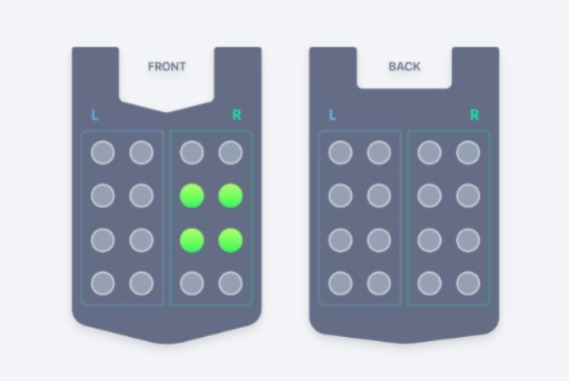
\includegraphics[width=\linewidth]{move_right_pattern.jpeg}   
\end{minipage}
\hfill
\begin{minipage}{0.49\textwidth}
    \centering
  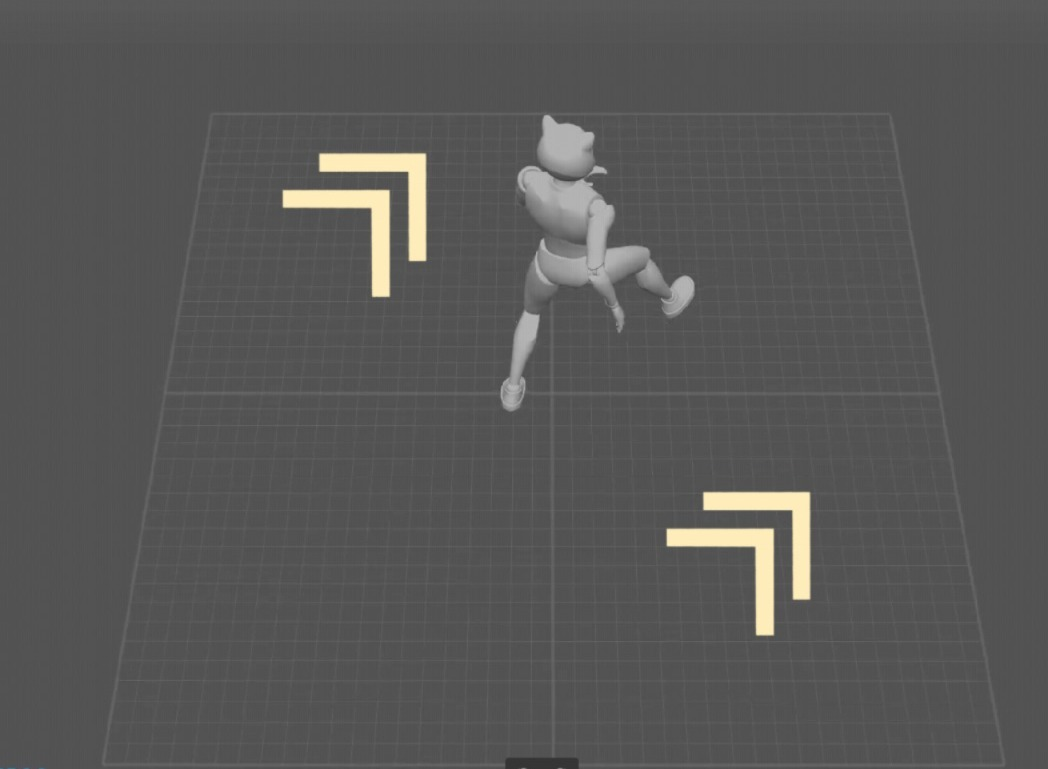
\includegraphics[width=\linewidth]{move_right_gif.jpeg}
\end{minipage}
\caption{"Move Right" signal's haptic pattern and visualization.}
\label{fig:move_right}
\end{figure}

\begin{figure}[H]
\centering
\begin{minipage}{0.49\textwidth}
    \centering
    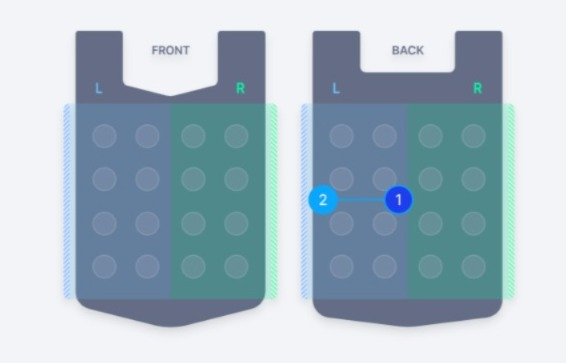
\includegraphics[width=\linewidth]{move_exact_left_pattern.jpeg}
\end{minipage}
\hfill
\begin{minipage}{0.49\textwidth}
    \centering
    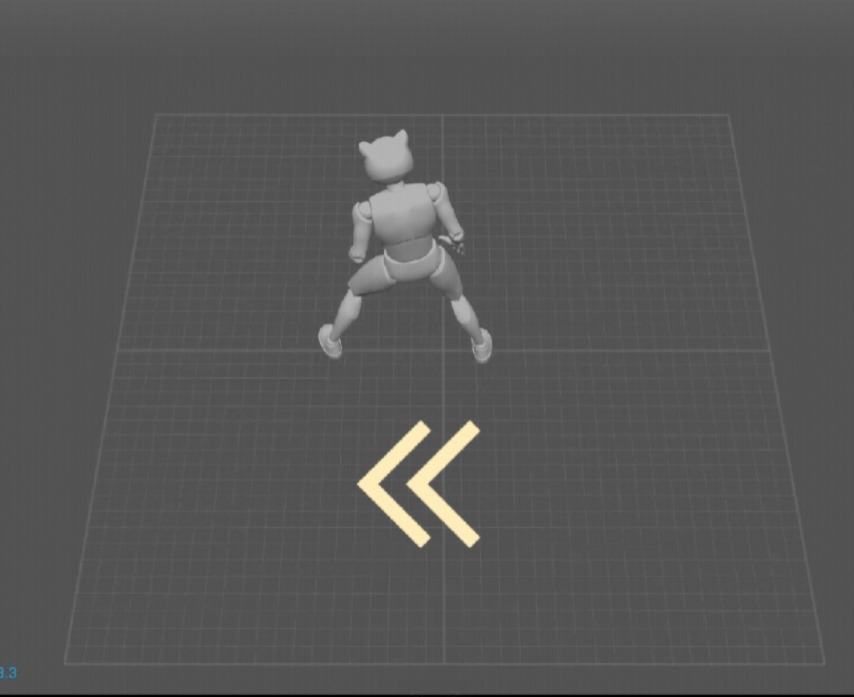
\includegraphics[width=\linewidth]{move_exact_left_gif.jpeg}
\end{minipage}
\caption{"Move Exact Left" signal's haptic pattern and visualization.}
\label{fig:move_exact_left}
\end{figure}

\begin{figure}[H]
\centering
\begin{minipage}{0.49\textwidth}
    \centering
    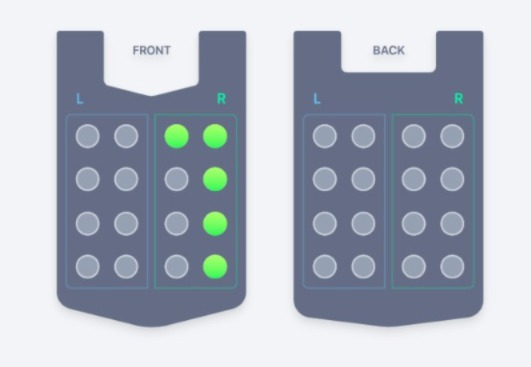
\includegraphics[width=\linewidth]{warning_right_front_pattern.jpeg}
\end{minipage}
\hfill
\begin{minipage}{0.49\textwidth}
    \centering
    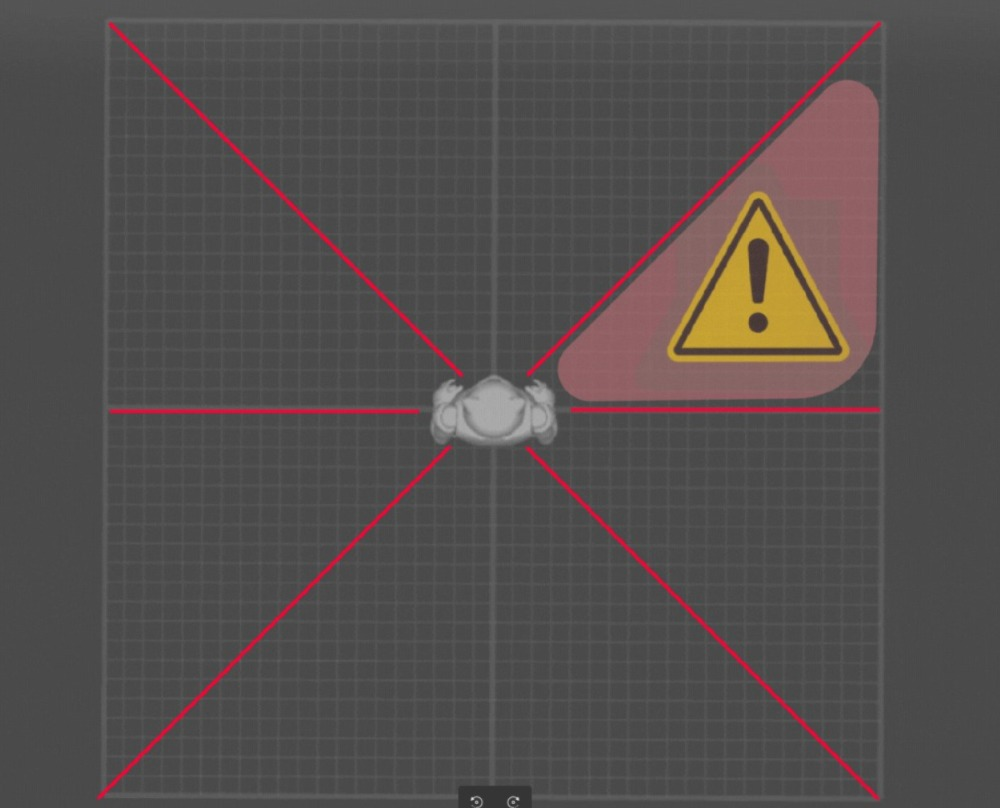
\includegraphics[width=\linewidth]{warning_right_front_gif.jpeg}
\end{minipage}
\caption{"Warning Right Front" signal's haptic pattern and visualization.}
\label{fig:warning_right_front}
\end{figure}

\subsubsection{Survey Design and Experimental Framework}

We completed the first phase ``Experiment 1 -- Signal Pattern Identification'' in which we systematically evaluate the haptic signals by focusing on:
\begin{itemize}
    \item identifying which signal patterns are more intuitive,
    \item analyzing the effect of intensity, and
    \item analyzing the effect of duration.
\end{itemize}

Throughout this process, we recorded objective performance metrics including reaction time (time between signal onset and first response), response time for final selection, and classification accuracy. Additionally, we logged whether the participant first identifies the direction or the signal category, allowing us to analyze the influence of response order on performance. After each trial, participants provided subjective evaluations using Likert-scale ratings, assessing factors such as confidence, clarity, perceived intensity, urgency, and comfort. These measurements allow us to evaluate not only the interpretability of each signal but also its cognitive load, usability, and user preference. The data collected in this phase plays a critical role in determining the mapping between haptic patterns and their intended meanings, as well as in selecting the most intuitive and distinguishable signal designs.

To collect user responses in a controlled and repeatable way, we developed a Python-based survey UI (\texttt{Tkinter}) with 3 blocks.

\begin{figure}[htbp]
    \centering
    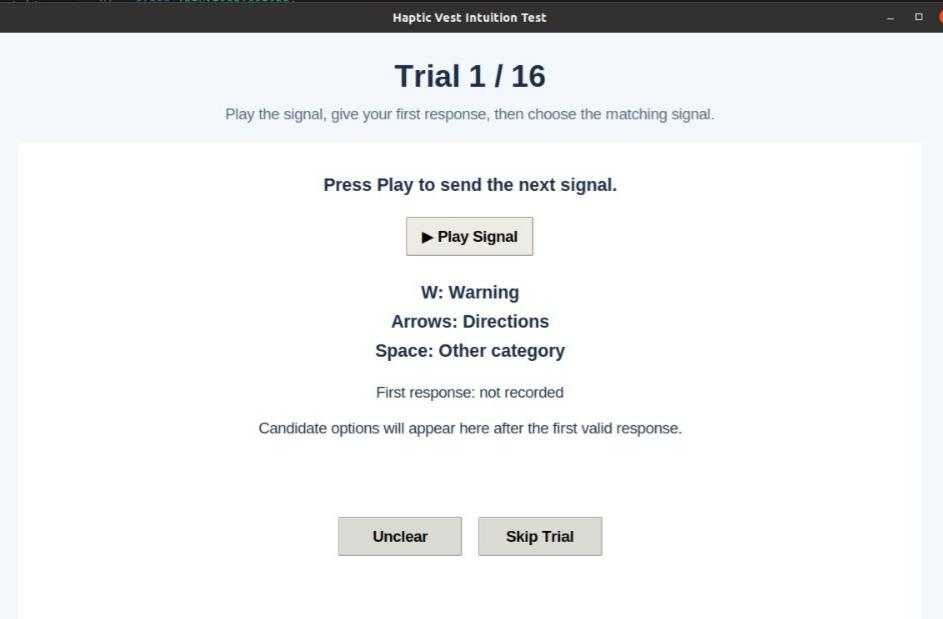
\includegraphics[width=\linewidth]{trial.jpg}
    \caption{Survey User Interface}
    \label{fig:trial0}
\end{figure}

\newpage

In the \textbf{intuition block}, the aim was to measure how the haptic signals are interpreted without training. Prior to the experiment, the visuals demonstrating the intended commands were shown and explained to the participants. They were informed about these commands' class [navigation, warning signal or movement modulation signal] without receiving the actual signal.

They were asked to classify the signal (\texttt{W/N}) and indicate direction using arrow keys. We recorded response time, classification accuracy, and direction accuracy, independent of which input (class or direction) was given first. After each trial, participants rated their confidence level, allowing us to also capture subjective perception. This block aims to measure haptic feedback's clarity and whether the patterns are intuitive to a person who does not know the exact pattern. After this first block, there was a training session in which the signal is sent to the vest while the user can see the pattern's visual on the vest and its intended command on the screen.

In the ``intensity'' and ``duration'' blocks, we applied the same signals with varying levels. Each signal was repeated with different intensities/durations to observe whether participants can distinguish them and how this affects:
\begin{itemize}
    \item response time,
    \item perceived urgency, and
    \item confidence.
\end{itemize}

\begin{figure}[H]
    \centering
    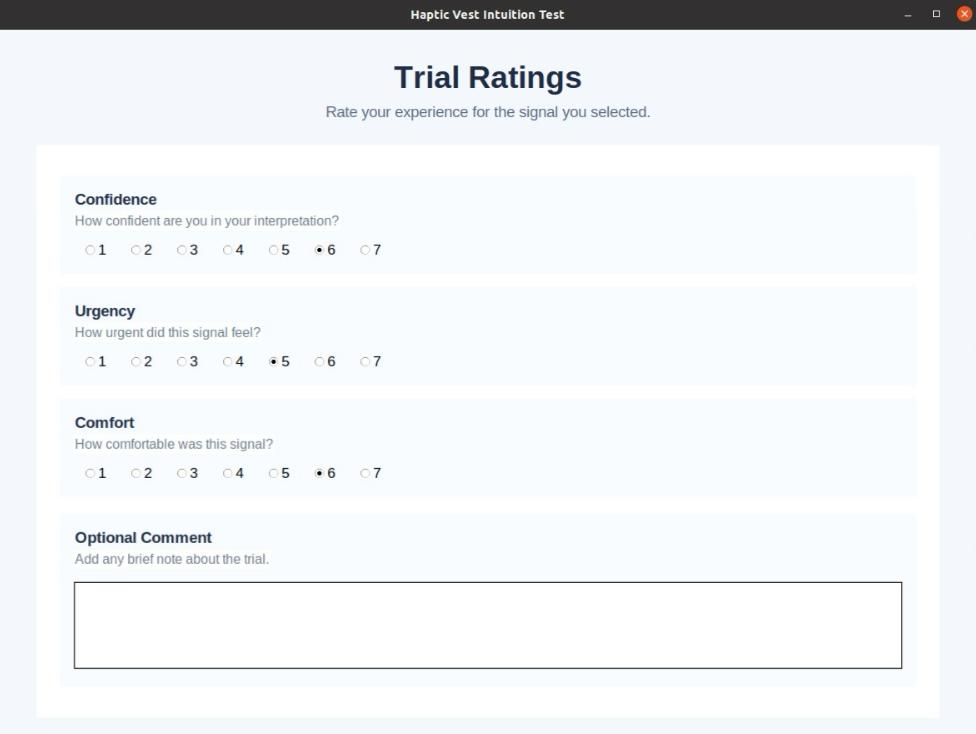
\includegraphics[width=\linewidth]{trial1.jpg}
    \caption{Survey User Interface}
    \label{fig:trial1}
\end{figure}

\begin{figure}[H]
    \centering
    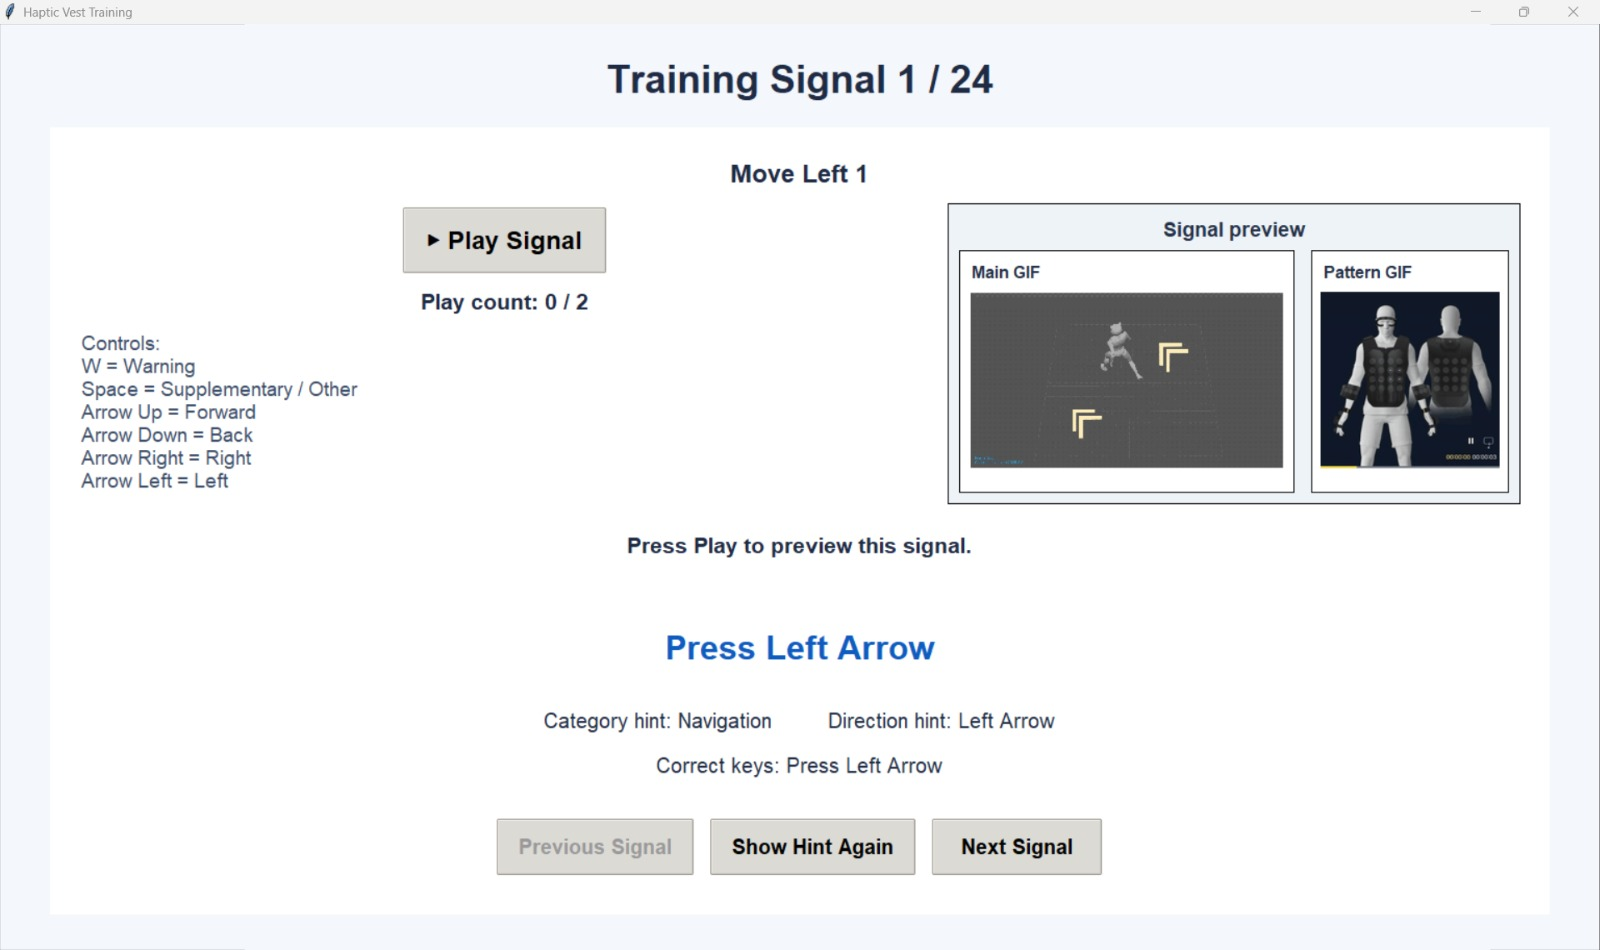
\includegraphics[width=\linewidth]{training_ui.jpeg}
    \caption{Survey User Interface - Training Block}
    \label{fig:Training ui}
\end{figure}

We also defined key evaluation metrics, including:
\begin{itemize}
    \item accuracy (direction and class identification),
    \item response time,
    \item perceived clarity and comfort,
    \item cognitive load, and
    \item improvement after training.
\end{itemize}

Finally, we set up the data logging pipeline, storing results in both \texttt{CSV} and Excel formats for later analysis. This includes detailed per-trial data such as response time, correctness, confidence rating (Likert scale 1-7), urgency rating (Likert scale 1-7), comfort rating (Likert scale 1-7), and signal type along with an optional comment block. The data were contained both in per-participant files and a master file for each block (intuition, intensity, duration) combining all participants' responses in single files to make the later analysis easier.

Overall, we established both the signal design space and a working experimental platform that allows us to systematically analyze how different haptic parameters affect human understanding of vibrotactile navigation cues.

\subsubsection{Performing the Survey}

Prior to the main user study, a pilot study was conducted to refine the haptic signal set through a preliminary evaluation. The design process consisted of three stages.

First, the design team conducted internal testing to verify signal functionality, identify implementation issues, and evaluate alternative signal designs. These sessions were used exclusively for iterative development and were not included in the final analysis.

Second, one external participant completed only the training block, which consisted of 36 signals, and provided qualitative feedback regarding signal distinguishability, comfort, and intuitiveness.

Finally, two external participants completed the full preliminary protocol, consisting of the intuition block (36 signals), training block (36 signals), duration block (50 signals), and intensity block (75 signals). The purpose of this pilot study was to compare alternative implementations of navigation and warning signals before finalizing the signal set used in the main experiment.

Several signals were represented by two or more candidate patterns. Examples included discrete versus continuous motion cues, alternative movement modulation patterns for on-track and off-track feedback, and different representations of self-centered and externally-centered rotational commands. The pilot study aimed to identify which signal variants were most intuitive, distinguishable, and comfortable.

\begin{table}[H]
\centering
\caption{Phase 1 Pilot Study Summary}
\label{tab:pilot_study}
\begin{tabular}{lcc}
\hline
\textbf{Preliminary Stage} & \textbf{Participants} & \textbf{Trial Count} \\
\hline
Training-only pilot & 1 & 24 \\
Intuition block & 2 & 72 \\
Duration block & 2 & 100 \\
Intensity block & 2 & 150 \\
\hline
\end{tabular}
\end{table}

Based on participant feedback and observed performance, the signal library was refined before the main study. In particular, non-coincident patterns were preferred for conceptually similar signals to improve discriminability. For example, when a discrete pattern was selected for a self-centered rotational cue presented from the front of the vest, a continuous sliding pattern was selected for the corresponding externally-centered rotational cue presented from the back. This design strategy reduced ambiguity between related navigation commands and improved overall signal differentiation.

\subsubsection*{Experimental Procedure}

The user study was conducted with 18 members (8 female, 10 male) from the Bo\u{g}azi\c{c}i University community, aged between 19 and 24 years. All participants in this stage were sighted; the study evaluates the perception and learnability of the vibrotactile vocabulary and does not constitute an evaluation with blind users. Participants had a mean height of 173.4 cm (median = 172.5 cm, range = 163--191 cm) and a mean weight of 67.7 kg (median = 65 kg, range = 50--94 kg). The participant pool was selected to represent a variety of body sizes, allowing the evaluation of the haptic vest across different physical characteristics. Before the experiment, participants were allowed to adjust the vest's side straps and shoulder snap fasteners to achieve an appropriate fit for their body size and shape.

Following the pilot study, the final signal set consisted of 24 haptic signals: 6 warning signals, 10 navigation signals, and 8 movement modulation signals. The complete experiment lasted approximately 45 minutes for each participant. In the intuition block, each of the 24 signals was presented once, followed by the training block.

The pilot study originally evaluated duration and intensity effects in two separate blocks. The duration block consisted of two different durations of the same signal, while the intensity block consisted of three different intensity levels. Based on observations from the pilot study, the final experiment combined these two blocks into a single mixed block containing 90 trials. To avoid unnecessary repetition, symmetric signal pairs were divided between the duration and intensity conditions. For example, \textit{Move Left}, \textit{Move Exact Right}, \textit{Robot-Centered Left Rotation}, and \textit{Self-Centered Right Rotation} were evaluated in the duration condition, whereas their symmetric counterparts (\textit{Move Right}, \textit{Move Exact Left}, \textit{Robot-Centered Right Rotation}, and \textit{Self-Centered Left Rotation}) were evaluated in the intensity condition. This approach reduced the total number of trials while maintaining coverage of all signal categories. The presentation order of signals was block-randomized independently for each participant. Consequently, every participant experienced a different trial sequence. Furthermore, signals representing different duration or intensity variants of the same command were never presented consecutively.

\begin{table}[H]
\centering
\caption{Phase 1 Main Experiment Summary}
\label{tab:phase1_summary}
\begin{tabular}{lc}
\hline
\textbf{} & \textbf{Number} \\
\hline
Participants & 18 \\
Male Participants & 10 \\
Female Participants & 8 \\
\hline
Intuition Block & 24 signals \\
Training Block & 24 signals \\
Mixed Block & 90 signals \\
Duration Trials & 36 (18 signals $\times$ 2 duration levels) \\
Intensity Trials & 54 (18 signals $\times$ 3 intensity levels) \\
\hline
\end{tabular}
\end{table}

\subsubsection{Data Collection and Statistical Analysis}

The collected data were analyzed at both the participant and signal levels. Performance metrics included signal recognition accuracy, response time, confidence, urgency, and comfort ratings. Analyses were conducted to evaluate learning effects, compare signal classes, investigate the influence of signal duration and intensity, identify common confusion patterns, and assess differences between signal categories such as warning, navigation, and movement modulation signals. Additional analyses examined directional recognition performance, front--back perception, continuous versus discrete signal designs, and the relationship between subjective ratings and objective recognition performance. Together, these analyses provide a comprehensive evaluation of the effectiveness, interpretability, and usability of the proposed haptic signal vocabulary. Prior to statistical analysis, the dataset was screened for data quality issues and response-time outliers. No implausible response times or extreme outliers were identified; therefore, all trials were retained. ``Don't Understand'' responses were treated as incorrect responses in accuracy analyses while retaining their subjective ratings. Response times were additionally normalized using participant-wise z-score normalization to reduce inter-participant variability. The outcomes of the statistical analyses are reported in the Results section alongside descriptive statistics, figures, and visualizations.

\paragraph{Wilcoxon Signed-Rank Test}
The Wilcoxon signed-rank test was used to compare two repeated conditions, such as warning versus navigation signals, duration level 1 versus duration level 2, and pre-training versus post-training performance. The test reports the signed-rank statistic $W$, the standardized test statistic $Z$, and the associated $p$-value. Statistical significance was accepted at $p < 0.05$. Effect size was calculated as
\[
r = \frac{|Z|}{\sqrt{N}},
\]
where $N$ denotes the number of paired observations. Following common conventions, effect sizes of approximately $0.1$, $0.3$, and $0.5$ were interpreted as small, medium, and large effects, respectively.

\paragraph{Friedman Test}
The Friedman test was used for repeated comparisons involving three or more levels, such as the three intensity levels. The test reports the Friedman chi-square statistic $\chi^2$ and the corresponding $p$-value. Effect size was quantified using Kendall's coefficient of concordance,
\[
W = \frac{\chi^2}{N(k-1)},
\]
where $N$ is the number of participants and $k$ is the number of repeated conditions. Values of approximately $0.1$, $0.3$, and $0.5$ were interpreted as small, medium, and large effects, respectively.

\paragraph{Post-hoc Analysis}
When a Friedman test revealed a significant overall effect, pairwise comparisons were performed using Wilcoxon signed-rank tests. Holm correction was applied to control the family-wise error rate associated with multiple comparisons.

\paragraph{Mann--Whitney U Test}
For comparisons between independent groups, such as male and female participants, the Mann--Whitney U test was employed. The test reports the $U$ statistic and the corresponding $p$-value. Effect size was quantified using Cliff's $\delta$.

\paragraph{Response Time Normalization}
To reduce inter-participant variability in baseline response speed, response times were normalized using participant-wise z-score normalization:
\[
z = \frac{x-\mu}{\sigma},
\]
where $x$ denotes the response time for a given trial, $\mu$ is the participant's mean response time, and $\sigma$ is the participant's response time standard deviation.

\subsection{Phase 2 - Path Tracking with Haptic Signals}

The first phase of the study focused on the design and evaluation of individual haptic signals. Based on the recognition accuracy, response time, confidence, comfort, and urgency analyses presented in Phase 1, the signal library was refined before proceeding to navigation experiments. Signals that produced low recognition performance, particularly several movement modulation cues, were redesigned. Furthermore, duration and intensity configurations that achieved the highest recognition accuracy were selected as the final signal parameters for navigation tasks.

While Phase 1 investigated whether participants could correctly interpret isolated haptic signals, Phase 2 evaluates whether these signals can be used to guide users through a physical environment. In this stage, participants are required to translate haptic feedback into navigation actions such as following a route, correcting their heading direction, recovering from path deviations, and avoiding nearby obstacles.

\begin{figure}[!ht]
    \centering
    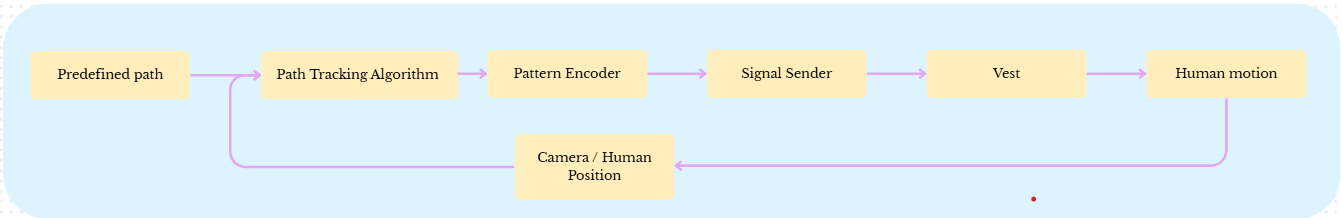
\includegraphics[width=1.0\linewidth]{phase2_diagram.png}
    \caption{Diagram for main structure of Phase 2.}
    \label{fig:phase2_diagram}
\end{figure}

Unlike the signal recognition experiments of Phase 1, effective navigation requires not only selecting appropriate haptic cues but also determining when each signal should be transmitted and how competing navigation objectives should be prioritized. Consequently, a signal encoding and signal sending framework was developed to continuously convert the user's position and orientation into navigation commands. The signal encoder determines which signal should be sent based on the user's current navigational context, while the signal sender decides when to transmit each signal. Together, these two components form the core of the Phase 2 navigation system.

To achieve this objective, a path-tracking encoder was developed. The encoder continuously maps the user's position and heading, relative to a route, into haptic navigation commands. The user pose is represented as
\[
x_h = (p,\theta),
\]
where $p=(x,y)$ denotes the user position and $\theta$ denotes the heading angle. At each control cycle, the encoder generates a haptic message
\[
m = (\text{signal},\text{mode}),
\]
where the transmitted signal depends on the current navigation state and the selected path-tracking strategy.

Four path-tracking strategies were designed and evaluated. The first strategy, Non-stop Waypoint Navigation, continuously guides the user while walking using directional haptic cues. The second, Stop-and-Align Navigation, prioritizes safety by requiring the user to stop and correct their orientation before continuing movement. The third, Hybrid Navigation, combines both approaches, aiming to balance the robustness of Stop-and-Align Navigation with the natural walking experience provided by Non-stop Waypoint Navigation. The fourth, Non-stop Align Navigation, targets smooth cornering: sharp route corners are replaced by curved local paths and the user is continuously pointed toward a look-ahead waypoint on the curve. The overall architecture of the Phase 2 navigation framework is illustrated in Figure~\ref{fig:phase2_diagram}.

Figures~\ref{fig:method1}--\ref{fig:method4} summarize the four strategies.

\begin{figure}[H]
\centering
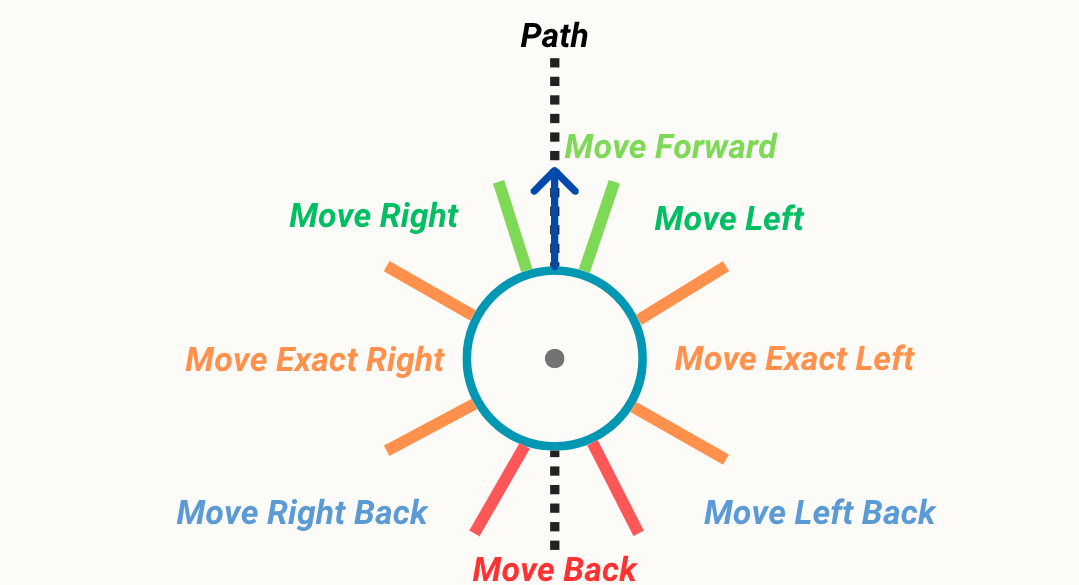
\includegraphics[width=0.8\linewidth]{figures/method_1_original_diagram.png}
\caption{Non-stop Waypoint Navigation direction regions. The heading error is mapped to one of eight haptic directions.}
\label{fig:method1}
\end{figure}

\begin{figure}[H]
\centering
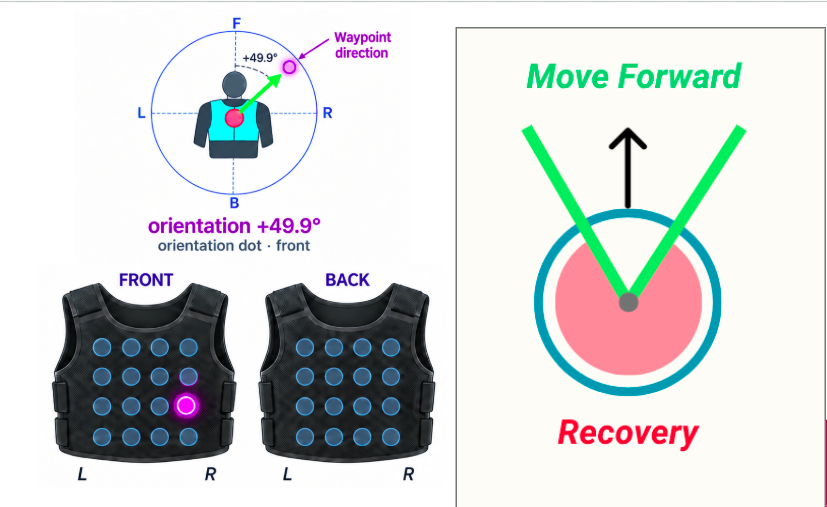
\includegraphics[width=0.85\linewidth]{figures/method_2_original_diagram.png}
\caption{Stop-and-Align Navigation. Left: the vest pointing vector toward the waypoint direction (orientation $+49.9^\circ$ in the example). Right: the move-forward margin and the recovery region.}
\label{fig:method2}
\end{figure}

\begin{figure}[H]
\centering
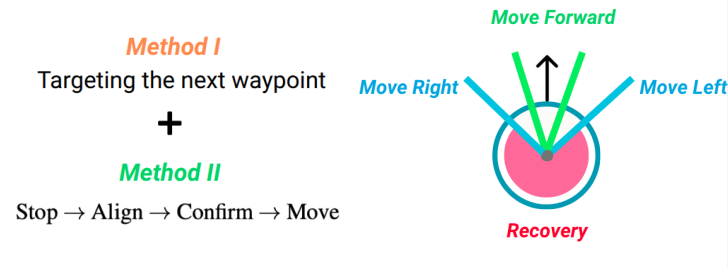
\includegraphics[width=0.85\linewidth]{figures/method_3_original_diagram.png}
\caption{Hybrid Navigation model, combining next-waypoint targeting with the stop-align-confirm-move sequence. Green: move forward; blue: move left/right while walking; red: stop and recovery.}
\label{fig:method3}
\end{figure}

\begin{figure}[H]
\centering
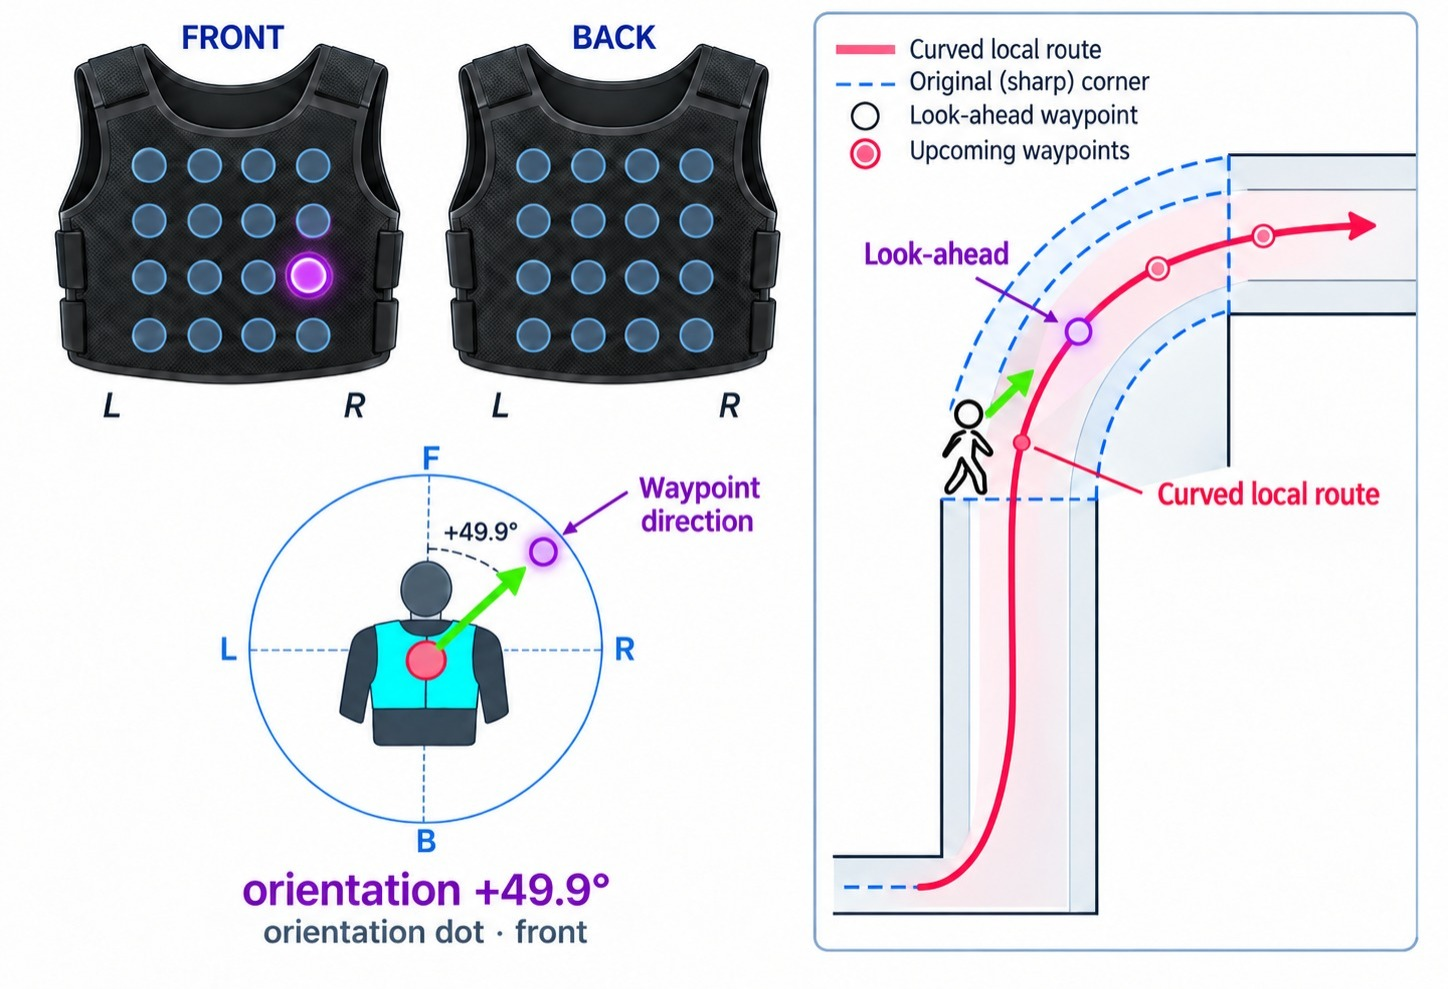
\includegraphics[width=0.9\linewidth]{figures/method_4_original_diagram.png}
\caption{Non-stop Align Navigation. The vest vector points toward a look-ahead waypoint placed on a curved local route that replaces the original sharp corner.}
\label{fig:method4}
\end{figure}

\subsubsection{Path Tracking Algorithms}

All three encoders share the same input, a state $x=(p,\theta)$ consisting of the user position $p=(p_x,p_y)$ and heading $\theta\in[0^\circ,360^\circ)$, and the same route, sampled at a fixed resolution $\delta_r$,
\[
T=\{p_0,p_1,\ldots,p_N\}.
\]
In the final system this route is produced by the path planner on the indoor map; during algorithm development, predefined trajectories were used. Each encoder is stateful and emits one haptic message per control step. They differ in how heading and position errors are converted into commands, but they share a common priority ordering in which obstacle warnings always dominate path-following,
\[
\text{Warning}
\succ
\text{Position Recovery}
\succ
\text{Orientation Recovery}
\succ
\text{Normal Navigation}.
\]

\paragraph{Obstacle warning model:}

The nearest obstacle is
\[
o^\ast=\arg\min_{o\in\mathcal{O}}\lVert o-p\rVert,
\]
where $\mathcal{O}$ is the set of detected obstacles (for circular obstacles the boundary distance $\lVert o-p\rVert-r_o$ is used). A warning is raised whenever $\lVert o^\ast-p\rVert\le d_{\text{warn}}$. The warning is two-tier:
\[
\begin{cases}
\lVert o^\ast-p\rVert \le d_{\text{crit}}, & \text{emergency stop},\\[4pt]
d_{\text{crit}} < \lVert o^\ast-p\rVert \le d_{\text{warn}}, & \text{directional warning}.
\end{cases}
\]
For a directional warning the relative bearing of the obstacle with respect to the user heading,
\[
\rho=\bigl(\operatorname{atan2}(o^\ast_y-p_y,\;o^\ast_x-p_x)-\theta\bigr)\bmod 360^\circ,
\]
is quantised into front / left-front / left-back / back / right-back / right-front sectors. While a warning is active no other command is issued, so obstacle avoidance overrides all path-following objectives.

\subsubsection*{Stop-and-Align Navigation}

The Stop-and-Align method prioritises safety and interpretability: orientation correction and position correction are never performed simultaneously, since walking while mis-oriented increases trajectory error and complicates signal interpretation. Navigation is decomposed into the sequence
\[
\text{Stop}\rightarrow\text{Align}\rightarrow\text{Confirm}\rightarrow\text{Move}
\]

When no warning is active, the closest point on the trajectory is obtained by segment projection, giving the closest segment index $i^\ast$ and the cross-track error
\[
d_{\text{traj}}=\min_{q\in T}\lVert q-p\rVert .
\]

\textbf{Position recovery:} If $d_{\text{traj}}>d_{\text{safe}}$ the user has left the safe corridor and position recovery is activated. Rather than steering toward the nearest path point, a recovery waypoint is placed ahead of the closest location,
\[
k=i^\ast+\left\lfloor \frac{\delta_{\text{wp}}}{\delta_r}\right\rceil ,
\]
where $\delta_{\text{wp}}$ is the look-ahead distance and $\lfloor\cdot\rceil$ denotes rounding to the nearest sample. The selection is corner-aware: if a detected corner lies between $i^\ast$ and $k$, the waypoint is snapped just beyond that corner, and if the candidate waypoint falls within $d_{\text{corner}}$ of a corner it is again advanced past it. The waypoint is clamped to the trajectory endpoint when necessary. Recovery itself is staged: the user is first told to stop and rotate to face the waypoint (\emph{Orientation\_start}), then to walk toward it (\emph{Position}); if the heading drifts while walking the user is re-aligned (\emph{Orientation\_on\_way}); and on arrival (within $d_{\text{reach}}$ of the waypoint) the heading is brought into line with the local path direction (\emph{Orientation\_end}). The recovery is re-planned if the user drifts laterally from the recovery line by more than $d_{\text{rec}}$, and it terminates early if the user crosses the trajectory at the waypoint.

\textbf{Orientation recovery and normal mode:} If the user is inside the corridor, the heading error relative to the local path direction $\psi_{i^\ast}$ is evaluated,
\[
\delta=\bigl(\psi_{i^\ast}-\theta\bigr)_{\pm 180^\circ}.
\]
A dual-threshold strategy with a hysteresis dead band is applied,
\[
\begin{cases}
|\delta|\le\alpha_{\text{align}}, & \text{aligned (move forward)},\\[4pt]
|\delta|>\alpha_{\text{stop}}, & \text{stop and rotate},\\[4pt]
\alpha_{\text{align}}<|\delta|\le\alpha_{\text{stop}}, & \text{maintain previous state},
\end{cases}
\]
where $\alpha_{\text{align}} < \alpha_{\text{stop}}$. The alignment threshold is intentionally chosen to be smaller than the stop threshold in order to enforce a stricter orientation requirement before forward motion is permitted. In other words, once the user enters the alignment mode, a more accurate heading must be achieved before the system considers the user aligned and resumes movement. This hysteresis region prevents rapid switching between alignment and movement states caused by small orientation fluctuations and improves the stability of the navigation guidance.

\subsubsection*{Non-stop Waypoint Navigation}

The Non-stop method provides a continuous walking experience: directional cues are issued while the user walks, without explicit stop-and-turn operations. At each step the closest trajectory point is found,
\[
p^\ast=\arg\min_{q\in T}\lVert q-p\rVert ,
\qquad
d_{\text{traj}}=\lVert p-p^\ast\rVert .
\]

\textbf{Inside the corridor:} ($d_{\text{traj}}\le d_{\text{safe}}$) the guidance does \emph{not} aim at the path tangent. A look-ahead point is taken on the centreline at arc length $s^\ast+d_{\text{look}}$ and then offset by the user's current lateral displacement, so the desired direction runs parallel to the route rather than pulling the user back to the centreline:
\[
w = c(s^\ast+d_{\text{look}}) + \bigl(p-p^\ast\bigr),
\qquad
\psi^\ast=\operatorname{atan2}\!\bigl(w_y-p_y,\;w_x-p_x\bigr),
\]
where $c(\cdot)$ is the centreline point at the given arc length. The heading error is
\[
\delta=\mathrm{wrap}_{(-180^\circ,180^\circ]}\!\bigl(\psi^\ast-\theta\bigr).
\]

\textbf{Outside the corridor} ($d_{\text{traj}}>d_{\text{safe}}$) the user enters recovery. A look-ahead recovery waypoint is selected at $s^\ast+d_{\text{look}}$ (advanced past an upcoming corner when one falls inside the look-ahead window), and the desired direction becomes the bearing toward it,
\[
\beta_w=\operatorname{atan2}\!\bigl(w_y-p_y,\;w_x-p_x\bigr),
\qquad
\delta=\mathrm{wrap}_{(-180^\circ,180^\circ]}\!\bigl(\beta_w-\theta\bigr).
\]
The recovery waypoint is held fixed across steps and re-selected only when the user drifts from the recovery line beyond $d_{\text{rec}}$ or reaches the current target.

In either case the heading error is mapped to one of eight discrete commands, each spanning a $45^\circ$ sector,
\[
\delta\;\longmapsto\;
\bigl\{\,
\text{forward},\ \text{left},\ \text{right},\ \text{exact-left},\
\text{exact-right},\ \text{back-left},\ \text{back-right},\ \text{back}\,
\bigr\},
\]
with \textit{forward} for $|\delta|\le 22.5^\circ$ and \textit{back} for $|\delta|\ge 157.5^\circ$. Commands are updated continuously according to the user's current orientation relative to either the offset look-ahead point (in corridor) or the recovery waypoint (in recovery). On reaching the final point a \textit{position achieved} signal is sent.

\subsubsection*{Hybrid Navigation}

The Hybrid method combines the natural walking of Non-stop Navigation with the robustness of Stop-and-Align: small errors are corrected while walking, whereas large errors or corridor departures trigger explicit recovery. At each step the encoder evaluates the cross-track error $d_{\text{traj}}$ and, inside the corridor, the heading error $\delta=(\psi_{i^\ast}-\theta)_{\pm 180^\circ}$ against three nested bands:
\[
\begin{cases}
|\delta|\le\alpha_{\text{fwd}}, & \text{move forward (continuous)},\\[4pt]
\alpha_{\text{fwd}}<|\delta|\le\alpha_{\text{stop}}, & \text{continuous left/right correction},\\[4pt]
|\delta|>\alpha_{\text{stop}}\ \text{or}\ d_{\text{traj}}>d_{\text{safe}}, & \text{stop-and-align recovery}.
\end{cases}
\]
While $|\delta|\le\alpha_{\text{stop}}$ and $d_{\text{traj}}\le d_{\text{safe}}$ the encoder behaves like the Non-stop method, issuing \textit{Move Forward} when the heading is within the forward band and steady \textit{Move Left} / \textit{Move Right} nudges otherwise, all without interrupting locomotion. The forward band can be narrowed adaptively with distance from the trajectory,
\[
\alpha_{\text{fwd}}(d_{\text{traj}})=
\alpha_{\text{fwd}}^{0}+\bigl(\alpha_{\text{fwd}}^{\,1}-\alpha_{\text{fwd}}^{0}\bigr)
\left(\min\!\Bigl(1,\tfrac{d_{\text{traj}}}{d_{\text{safe}}}\Bigr)\right)^{\!\gamma},
\]
so that tolerance tightens as the user approaches the corridor boundary.

Once the heading error exceeds $\alpha_{\text{stop}}$ or the user leaves the corridor, the encoder switches to the Stop-and-Align recovery logic described above (stop and rotate, or staged position recovery), returning to continuous guidance only after alignment falls back below $\alpha_{\text{align}}$. By adaptively switching between the two strategies, the Hybrid method balances navigation efficiency, path-tracking accuracy, safety, and user comfort.

\subsubsection*{Non-stop Align Navigation}

The fourth method addresses a weakness observed in the other strategies at route corners. When a route turns sharply, a user who follows the discrete corner is either told to stop and rotate (Stop-and-Align) or receives abrupt direction changes that can cause overshoot and zig-zag motion (Non-stop Waypoint and Hybrid). Non-stop Align Navigation keeps the user walking and reduces these effects by smoothing the route itself.

Sharp corners of the route $T$ are replaced by a curved local path $\tilde{T}$ around each detected corner. A look-ahead waypoint $w_{\text{la}}$ is selected on this curved path ahead of the user's closest point, and the vest vector, i.e., the continuously updating pointing signal also used for orientation recovery, indicates the direction of $w_{\text{la}}$ relative to the user's heading,
\[
\delta=\mathrm{wrap}_{(-180^\circ,180^\circ]}\!\bigl(\operatorname{atan2}(w_{\text{la},y}-p_y,\;w_{\text{la},x}-p_x)-\theta\bigr).
\]
As the user advances, the look-ahead waypoint moves along the curve, so the indicated direction rotates gradually and the user steers smoothly through the corner rather than receiving a sudden turn command. The obstacle warning priority of the other methods is unchanged. The goal of this strategy is to reduce overshoot and zig-zag motion at corners while preserving continuous walking.

\subsubsection*{Overview of the Signals}
The output of the signal encoder that is transmitted to the haptic vest for each path-tracking algorithm is listed in Table~\ref{tab:algorithm_signals}.

When the encoder transmits the continuous \textit{Angle Difference} signal during orientation recovery, it functions as a virtual haptic compass needle. Utilizing the bHaptics \texttt{play\_path} function, the system generates a localized point of vibration at a fixed vertical height on the vest. As the user physically rotates, this focal point of vibration pans smoothly across the torso, transitioning seamlessly between the front and back panels to continuously indicate the relative direction of the target heading. Once the user's orientation falls within the predefined alignment margin, this dynamic tracking ceases, and a discrete \textit{On Track} confirmation signal is transmitted to indicate successful orientation alignment.

\begin{table}[H]
\centering
\caption{Signals Transmitted per Navigation Algorithm Case}
\label{tab:algorithm_signals}
\begin{tabular}{@{}p{3.5cm} p{5.0cm} p{6.0cm}@{}}
\toprule
\textbf{Algorithm} & \textbf{Navigation Case} & \textbf{Signals Transmitted} \\
\midrule
\textbf{Stop-and-Align} 
& Normal Mode (Aligned) & ``Move Forward'', ``On Track'' \\
& Orientation Recovery (Misaligned) & ``Stop'', Angle Difference, ``On Track'' \\
& Position Recovery (Outside Corridor) & ``Stop'', Angle Difference, ``Move Forward'', ``On Track'' \\
& Obstacle Warning & Directional Warnings, ``Stop''\\
\midrule
\textbf{Non-stop Waypoint} 
& Continuous Tracking (8-Sector) & ``move\_forward'', ``move\_left'', ``move\_right'', ``move\_exact\_left'', ``move\_exact\_right'', ``move\_back\_left'', ``move\_back\_right'', ``move\_back'' \\
& Goal Reached & ``On\_Track'' \\
& Obstacle Warning & Directional Warnings, ``emergency\_stop'' \\
\midrule
\textbf{Hybrid (Version 3)} 
& Normal Mode (Inner Band) & ``Move Forward'', ``On Track'' \\
& Normal Mode (Middle Band) & ``Move Left'', ``Move Right'' \\
& Orientation Recovery (Outer Band) & ``Stop'', Angle Difference, ``On Track'' \\
& Position Recovery (Outside Corridor) & ``Stop'', Angle Difference, ``Move Forward'', ``On Track'' \\
& Obstacle Warning & Directional Warnings, ``Stop'' \\
\midrule
\textbf{Non-stop Align}
& Continuous Tracking (Curved Local Path) & Angle Difference (continuous pointing vector toward look-ahead waypoint) \\
& Goal Reached & ``Position Achieved'' \\
& Obstacle Warning & Directional Warnings, ``Stop'' \\
\bottomrule
\end{tabular}
\end{table}

\subsubsection{Signal Sender}

The signal sender governs when each signal selected by the encoder is actually transmitted, operating according to two complementary policies: case-based and time-based. Under the case-based policy, signals tied to safety-critical or momentary navigational events --- warnings, orientation-alignment cues, and interrupt signals such as on-track confirmations, emergency stops, and position/orientation-achieved notifications --- are transmitted immediately as soon as the corresponding case is detected, ensuring the user receives time-sensitive feedback without delay. Under the time-based policy, by contrast, movement-guidance signals (e.g., move forward, move left/right) follow an explicit play-and-wait cycle: each signal is played once for a fixed duration and then withheld for a configurable repeat interval before being reissued, so the user is guided continuously without being overwhelmed by uninterrupted haptic stimulation. This time-gated behavior is further refined by a signal-stability threshold, which only accepts a new movement signal once the encoder has requested it consistently for a minimum duration --- filtering out transient flicker --- and by turning-point overrides, which allow an imminent directional change near a path corner to interrupt the current timing cycle and be communicated immediately. Together, these case-based and time-based mechanisms allow the signal sender to deliver critical cues instantly while pacing routine guidance signals in a way that supports a natural and comfortable navigation experience.

\subsubsection{Simulation Environments}

Before conducting the physical navigation experiments, we developed both two-dimensional and three-dimensional simulation environments to validate the proposed path-tracking algorithms, signal encoder, and signal sender framework. These simulation platforms enabled us to test the overall navigation pipeline, identify potential implementation issues, and collect preliminary user feedback before proceeding to real-world experiments.

\subsubsection*{2-D Simulations}

As an initial validation step, we developed a two-dimensional simulation environment using the \texttt{Matplotlib} library. At this stage, the signal sender module was not yet integrated, and the primary objective was to evaluate the behavior of the Stop-and-Align and Hybrid navigation algorithms; the Non-stop Align method was added to the same framework afterwards.

The simulation allowed users to navigate through predefined paths using keyboard arrow keys while visualizing the real-time outputs generated by the signal encoder. The interface consisted of two main panels. The left panel displayed the user's current position, orientation, predefined trajectory, and safety margins, enabling detailed observation of the path-tracking behavior. The right panel visualized the vibrotactile patterns that would be transmitted to the haptic vest, allowing us to verify the correctness and timing of the generated navigation cues (as in Figures~\ref{fig:stop_and_align_2d_sim}, \ref{fig:hybrid_2d_sim}, \ref{fig:Recovery_2d_sim}).

This environment provided a rapid prototyping platform for debugging the navigation algorithms and evaluating their performance under various path configurations.

\begin{figure}[H]
\centering
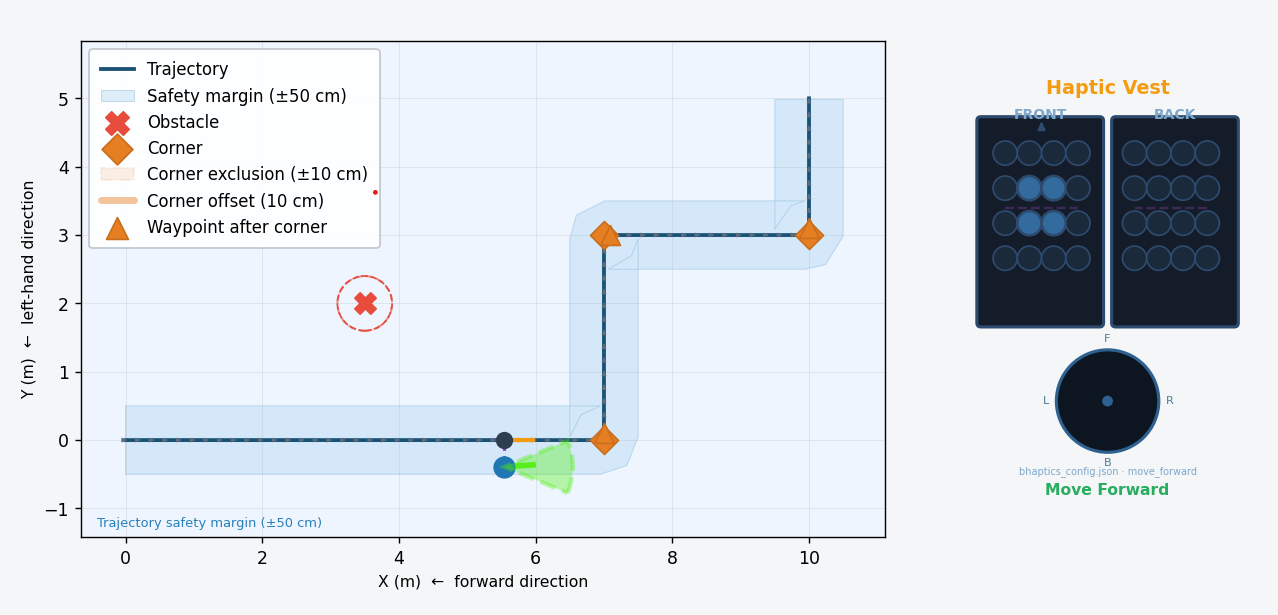
\includegraphics[width=\linewidth]{stop_align_2d_sim.png}
\caption{Stop and Align 2-D Sim. Character is represented with the blue dot, and the green cone depicts the \textit{Move Forward} margin.}
\label{fig:stop_and_align_2d_sim}
\end{figure}

\begin{figure}[H]
\centering
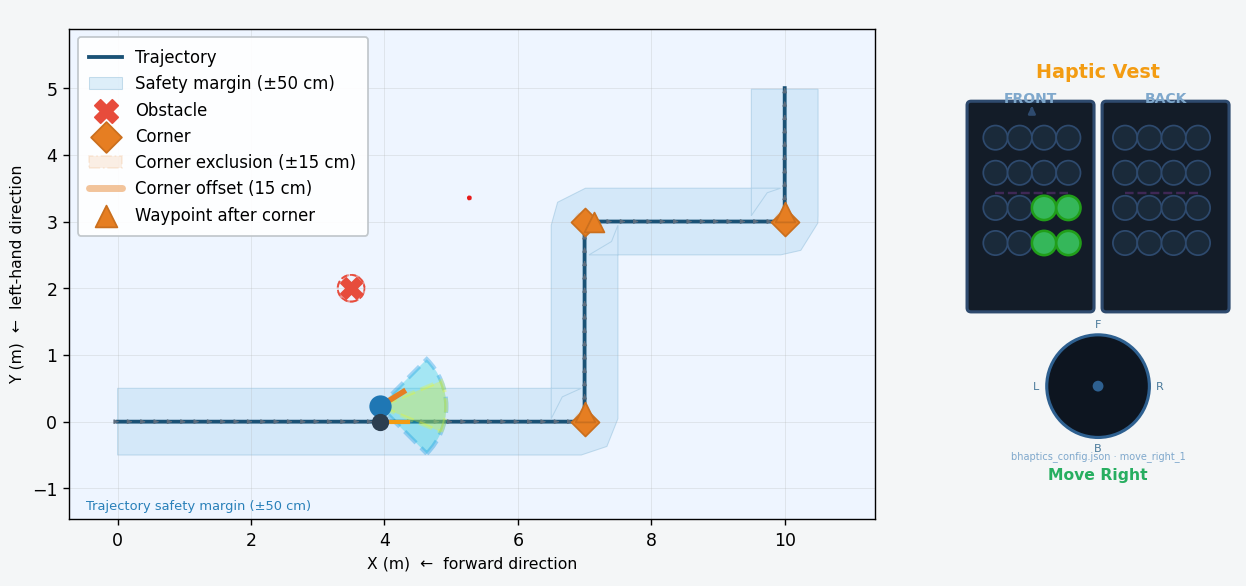
\includegraphics[width=\linewidth]{hybrid_2d_sim.png}
\caption{Hybrid Model 2-D Sim. Character is represented with the blue dot. While the blue cone depicts the \textit{Move Left} and \textit{Move right} margin, yellow cone depicts the \textit{Move Forward} margin.}
\label{fig:hybrid_2d_sim}
\end{figure}

\begin{figure}[H]
\centering
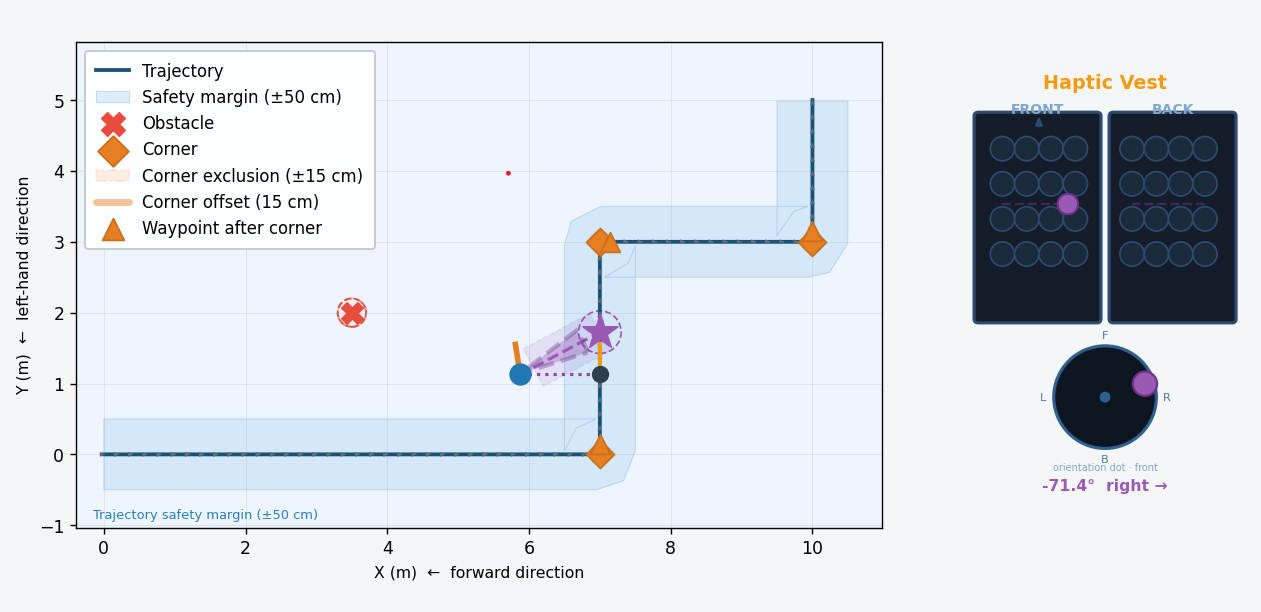
\includegraphics[width=\linewidth]{Recovery_2d_sim.png}
\caption{Recovery Mode Model for 2-D Sim. Alignment margin is represented with purple cone.}
\label{fig:Recovery_2d_sim}
\end{figure}

\subsubsection*{3-D Simulations}

To further evaluate the proposed framework and obtain feedback from external users, a three-dimensional simulation environment was developed using \texttt{VisPy}. Unlike the 2-D simulation, this platform incorporated both the signal sender module and the vibrotactile haptic vest, enabling end-to-end testing of the complete guidance pipeline.

Participants navigated through predefined paths in the virtual environment using an Xbox controller while receiving haptic guidance through the vest. Their objective was to complete the assigned trajectories as accurately as possible using only the generated haptic feedback.

The simulation was designed with three synchronized displays. The primary display presented the user's perspective within the virtual environment (as in Fig.~\ref{fig:Participant_view}). Two additional administrative panels were developed for monitoring purposes. The first admin panel visualized the vibration patterns currently being transmitted to the haptic vest (as in Fig.~\ref{fig:Admin_view_vest}), while the second displayed the participant's real-time position, orientation, trajectory, and safety margins (as in Fig.~\ref{fig:Admin_view_visualization}). These monitoring tools enabled detailed observation of the system's behavior and facilitated debugging and performance evaluation.

The 3-D simulation served as an important intermediate step between algorithm development and real-world experiments, allowing us to assess usability, collect user feedback, and refine the navigation framework before deploying it in physical environments.

\begin{figure}[H]
\centering
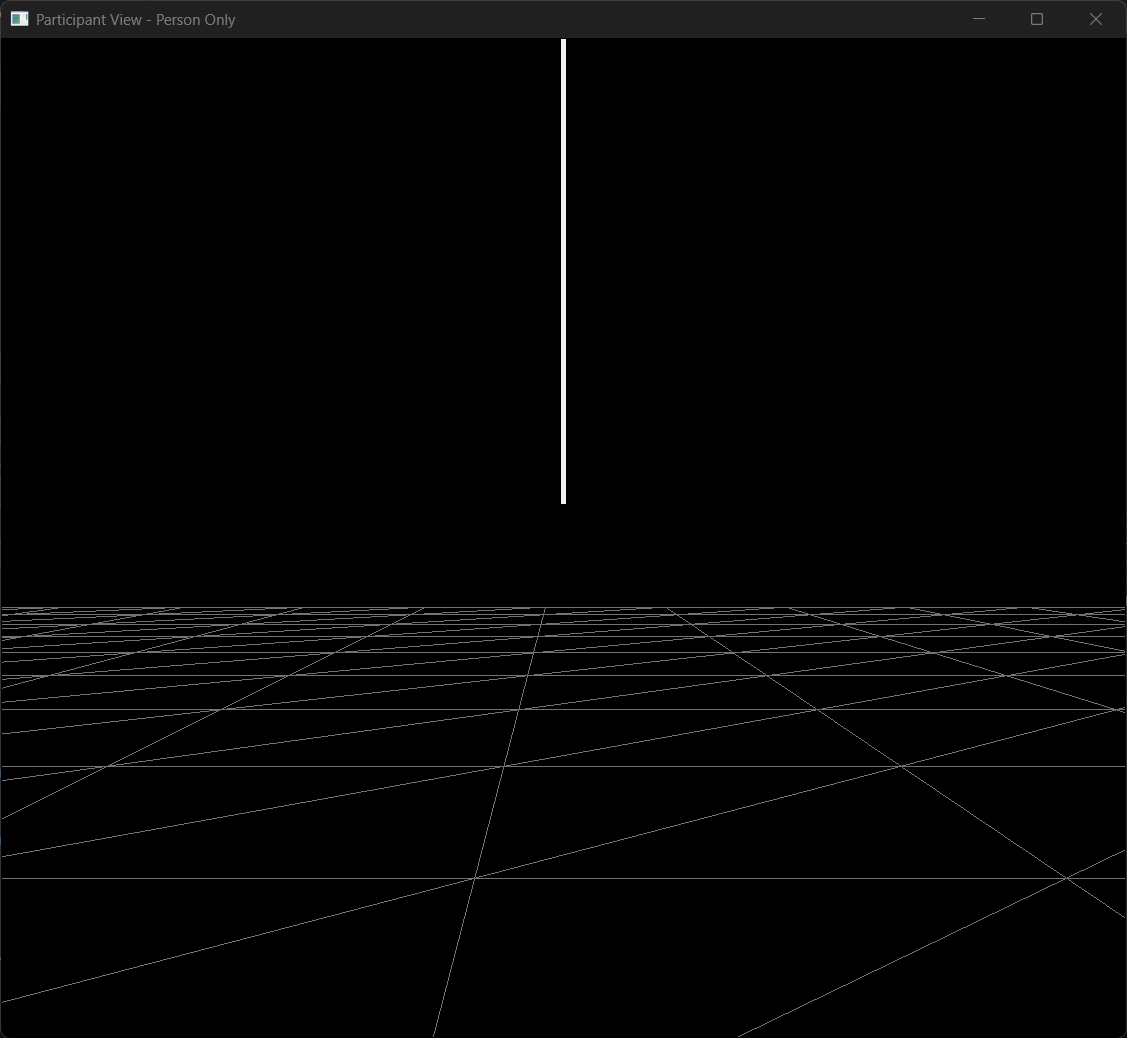
\includegraphics[width=300pt]{Participant_view.png}
\caption{Participant View in 3-D Sim.}
\label{fig:Participant_view}
\end{figure}

\begin{figure}[H]
\centering
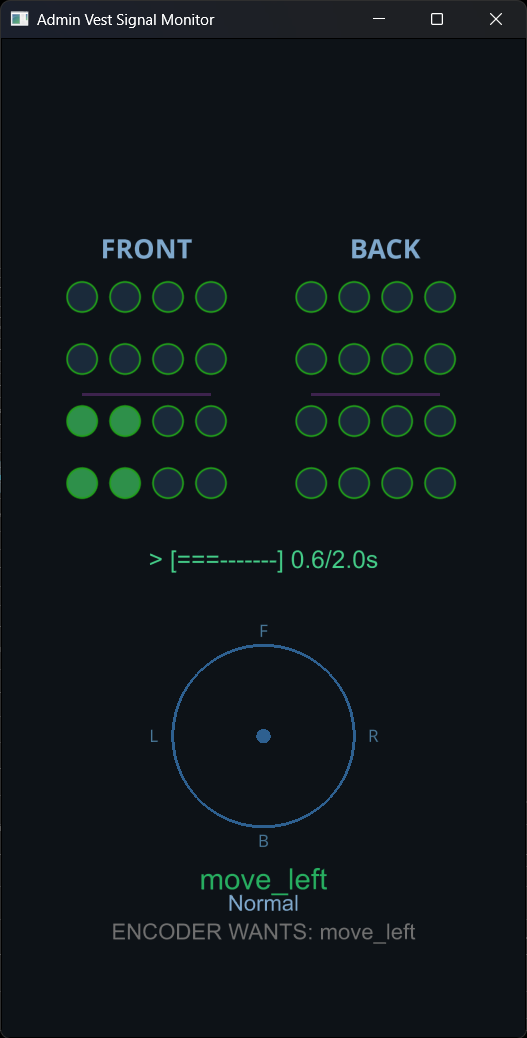
\includegraphics[width=150pt]{Admin_view_vest.png}
\caption{Admin View Vest Panel in 3-D Sim.}
\label{fig:Admin_view_vest}
\end{figure}

\begin{figure}[H]
\centering
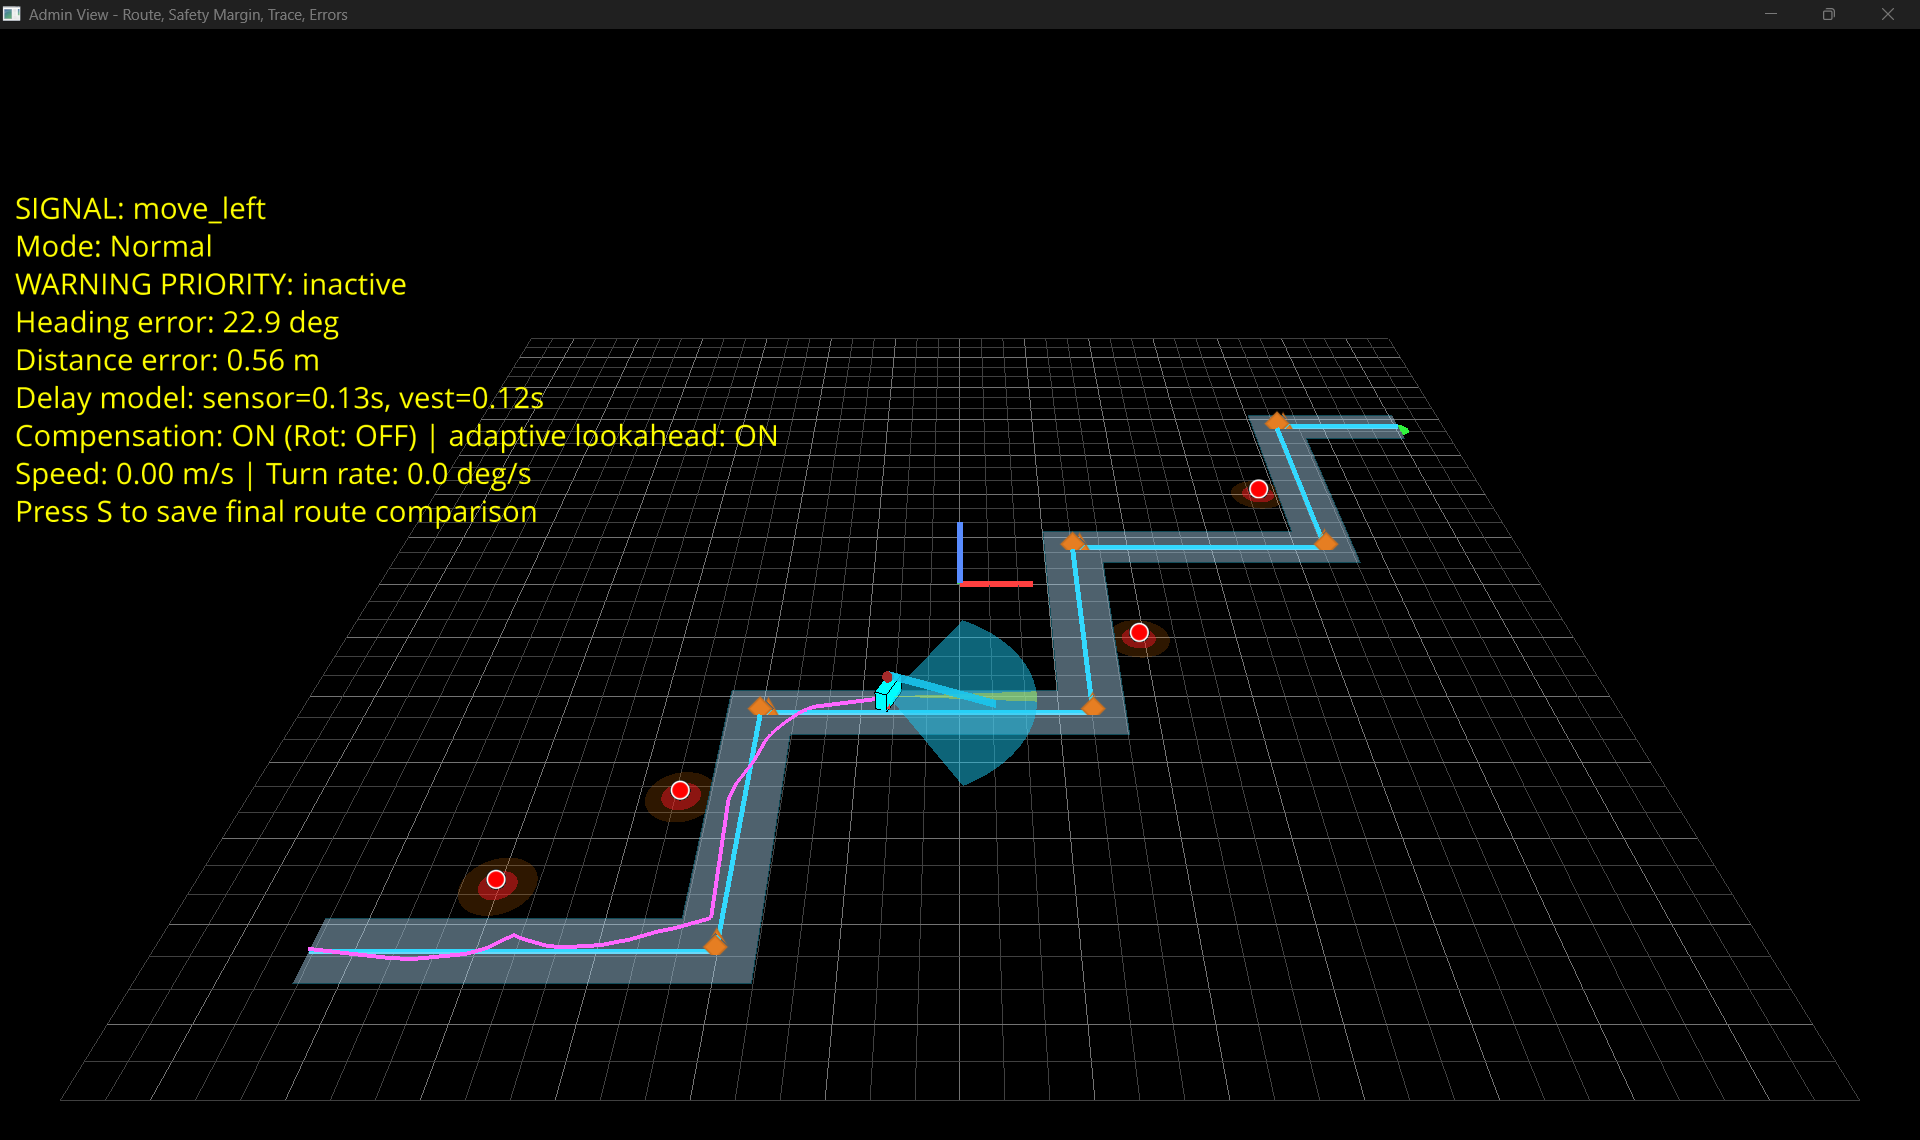
\includegraphics[width=\linewidth]{Admin_view_visualization.png}
\caption{Admin View Visualization Panel in 3-D Sim.}
\label{fig:Admin_view_visualization}
\end{figure}

\subsubsection*{Camera Integration}

Human position and orientation tracking is implemented using a ZED 2 stereo camera, as shown in Fig.~\ref{fig:zed2_camera}. Although the tracking system is still under active development and several limitations remain, the camera has been successfully integrated into the simulation framework.

The tracking data are continuously streamed to the navigation system and used to estimate the participant's position and heading in real time. This integration enables realistic simulation of human navigation behavior and allows the complete haptic guidance framework to be evaluated under conditions that closely resemble the intended physical experiments. The same camera will subsequently serve as the source for indoor mapping and localization in the full navigation system.

\begin{figure}[H]
\centering
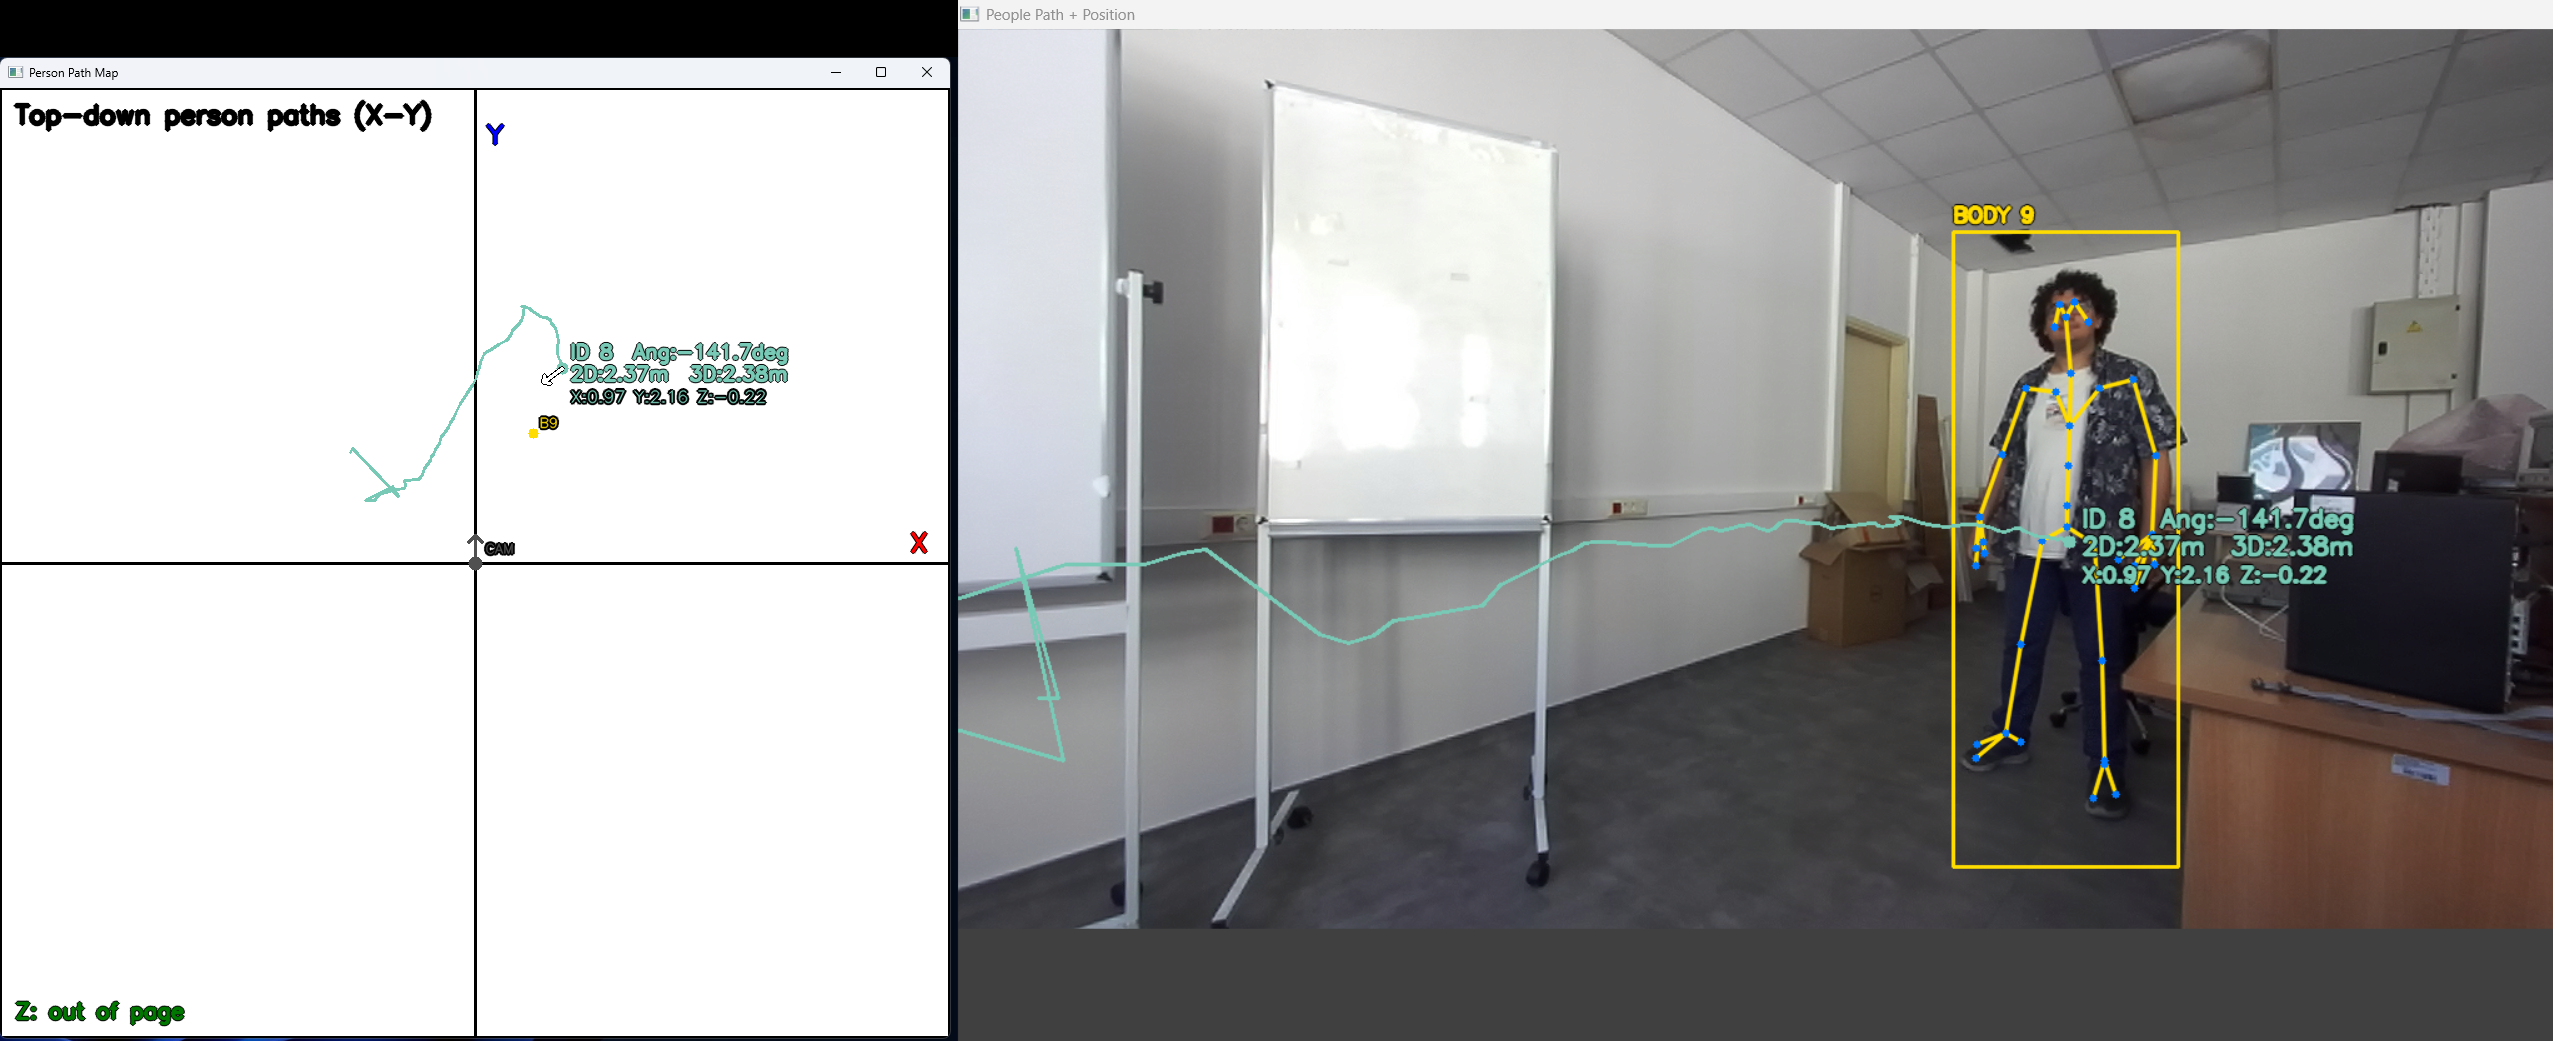
\includegraphics[width=\linewidth]{zed2_implementation.png}
\caption{ZED 2 Camera Implementation.}
\label{fig:zed2_camera}
\end{figure}

\subsubsection*{Path Selection}

Three different navigation paths were designed for the user study in order to evaluate the proposed path-tracking algorithms under varying levels of difficulty.

The first path was designed as an easy trajectory consisting primarily of $45^\circ$ and $90^\circ$ turns. The second path incorporated more complex turning angles and directional changes to increase navigational difficulty. Finally, the third path was designed to pass close to obstacles, requiring more frequent corrective actions and providing a greater opportunity to evaluate the effectiveness of the obstacle warning signals and safety mechanisms.

Together, these three trajectories allow the evaluation of the navigation framework across a range of realistic indoor navigation scenarios, including straight segments, turns, and obstacle proximity.

\subsubsection*{Planned Navigation Study}

The planned navigation study consists of evaluating all four path-tracking algorithms on each of the three predefined trajectories, resulting in a total of twelve experimental conditions. The first path, with its $45^\circ$ and $90^\circ$ turns, and the second, with more complex turning angles, are particularly informative for comparing the corner behavior of Non-stop Align Navigation against the other methods.

During the experiment, participants will wear the vibrotactile haptic vest and will be continuously tracked using the camera-based localization system. Participants will be instructed to follow the designated trajectories using only the haptic feedback provided by the navigation framework. Early feasibility experiments may involve sighted participants under controlled visual restriction; results from such trials will be reported separately and will not be treated as equivalent to evaluation with blind users. Experiments involving blind participants will be conducted only with appropriate recruitment procedures, accessible instructions, supervision, safety measures, and the required institutional approval. Trials will take place in a supervised, obstacle-controlled space with an accessible stop mechanism and a nearby experimenter. Trial order will be counterbalanced where possible to reduce learning effects, and participants will receive structured training with the selected vibration patterns before the navigation trials.

Performance will be assessed using objective navigation metrics such as task completion rate, trajectory deviation (cross-track error), path completion time, travelled distance, heading error, wrong turns, stopping events, the number of corrective actions, and obstacle-related interventions. In addition, subjective feedback regarding comfort, intuitiveness, workload, confidence, and overall user experience will be collected through post-experiment questionnaires. Acceptance thresholds will be established after pilot testing and fixed before the main study, and comparative results will be reported with variability and appropriate statistical analysis, without assuming that any strategy will be superior.

The collected data will be used to compare the effectiveness of the Non-stop Waypoint, Stop-and-Align, Hybrid, and Non-stop Align navigation strategies and to identify the most suitable approach for conveying navigation instructions to blind users through vibrotactile feedback.

%% ============================================================
%%  CHAPTER 5 — CONCLUSION
%% ============================================================
\setcounter{section}{5}
\setcounter{subsection}{0}
\setcounter{subsubsection}{0}
\chapter*{\centering CHAPTER 5\\[4pt]RESULTS AND CONCLUSION}
\addcontentsline{toc}{chapter}{5. RESULTS AND CONCLUSION}
\thispagestyle{fancy}

\subsection{Results}
This section presents the results of the Phase 1 user study conducted to evaluate the proposed haptic signal vocabulary. The findings are organized according to the main research questions, including signal recognition performance, training effects, signal design comparisons, and the influence of signal parameters such as duration and intensity. Descriptive statistics, visualizations, and statistical analyses are provided to support the interpretation of the results.

\subsubsection*{Learning Effects and Training Analysis}

The training block was designed to familiarize participants with the signal library. All 24 signals were presented together with their visual demonstrations. Participants were allowed to replay the signals using an on-screen play button and review the demonstrations at their own pace. Questions regarding signal meanings and navigation concepts were answered during this phase. After the training block, users moved on to the mixed block consisting of 90 trials. To reduce cognitive fatigue, a mandatory five-minute break was introduced after the 45th trial of the block. Figure~\ref{fig:learning_curve} illustrates the evolution of participant accuracy throughout the experiment. A rapid increase in accuracy can be observed during the first few trials of the pre-training intuition block, indicating a short familiarization period. During the mixed block, performance initially remains relatively stable before gradually decreasing as participants approach the middle of the block, suggesting the effects of cognitive fatigue. Following the mandatory break, accuracy levels increase again, indicating that the rest period helped participants maintain attention and performance throughout the remainder of the experiment.

\begin{figure}[H]
\centering
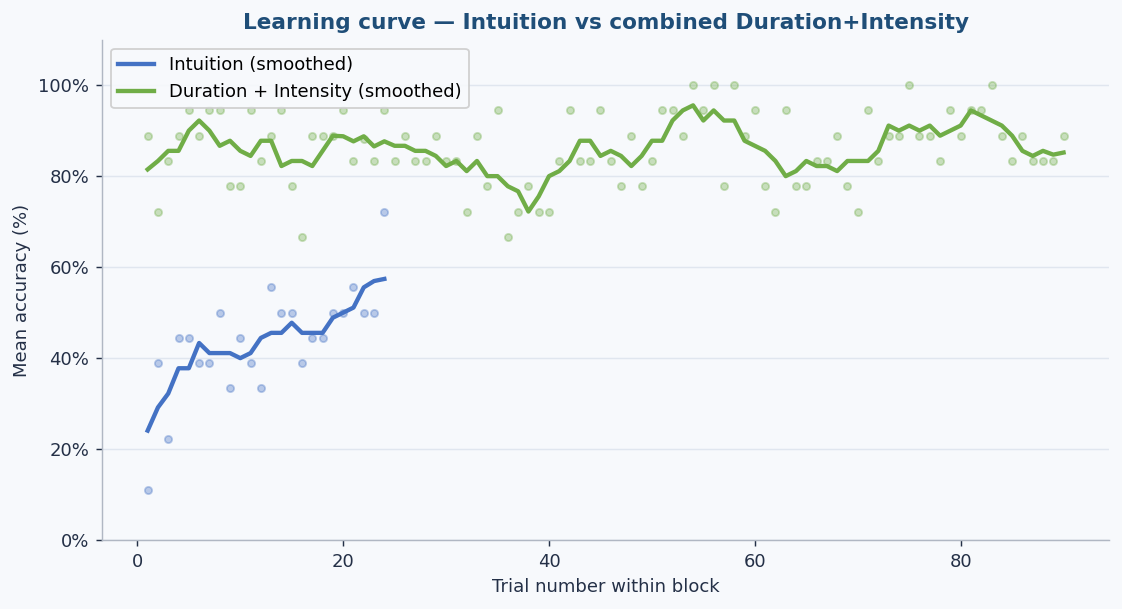
\includegraphics[width=0.85\linewidth]{learning_curve.png}
\caption{Average accuracy for each trial number.}
\label{fig:learning_curve}
\end{figure}

To evaluate the effectiveness of the training procedure, participant performance in the pre-training intuition block was compared with performance in the combined duration and intensity blocks. For each participant, mean accuracy, confidence rating, and response time were calculated. Since the measurements were paired and normality could not be assumed, Wilcoxon signed-rank tests were used for statistical comparisons.

\begin{figure}[H]
    \centering
    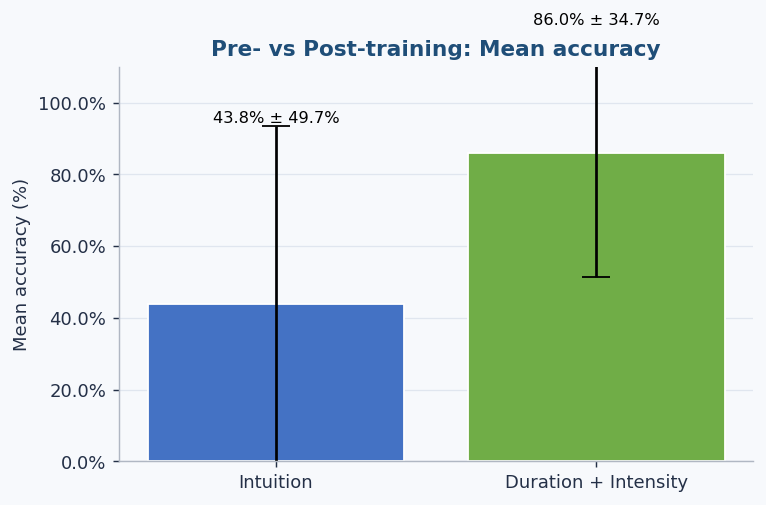
\includegraphics[width=0.8\linewidth]{training_effect_accuracy.png}
    \caption{Mean signal recognition accuracy before and after training.}
    \label{fig:training_effect_accuracy}
\end{figure}

As shown in Figure~\ref{fig:training_effect_accuracy}, signal recognition accuracy increased substantially after training. Mean accuracy improved from $43.8 \pm 49.7\%$ during the intuition block to $86.0 \pm 34.7\%$ in the post-training blocks, corresponding to an absolute improvement of 42.2 percentage points ($p = 7.63 \times 10^{-5}$, $r = 0.85$). This result indicates that participants were able to learn and recognize the haptic signals considerably more accurately after becoming familiar with the signal set.

\begin{figure}[H]
    \centering
    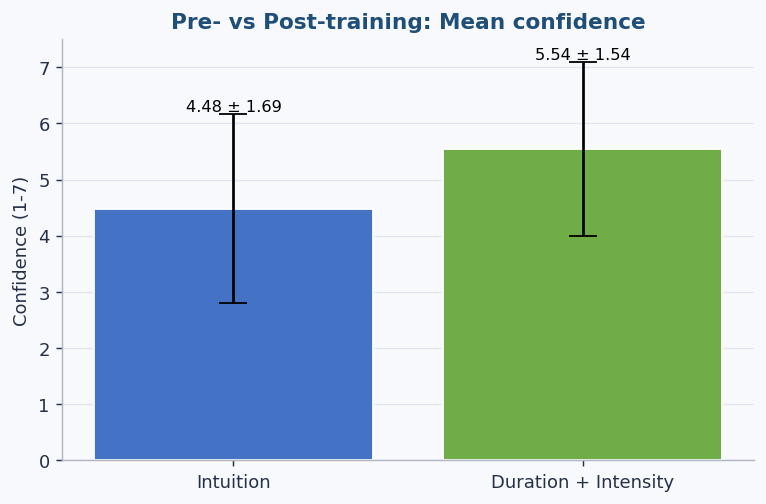
\includegraphics[width=0.8\linewidth]{training_effect_confidence.png}
    \caption{Mean confidence ratings before and after training.}
    \label{fig:training_effect_confidence}
\end{figure}

Participant confidence also increased following training, as illustrated in Figure~\ref{fig:training_effect_confidence}. The mean confidence rating increased from $4.48 \pm 1.69$ to $5.54 \pm 1.54$ on the 1--7 Likert scale, representing a relative increase of approximately 23.7\% (Wilcoxon signed-rank test, $p = 3.81 \times 10^{-5}$, $r = 0.88$). The increase in confidence suggests that participants became more certain about their interpretations of the haptic cues after training.

\begin{figure}[!ht]
    \centering
    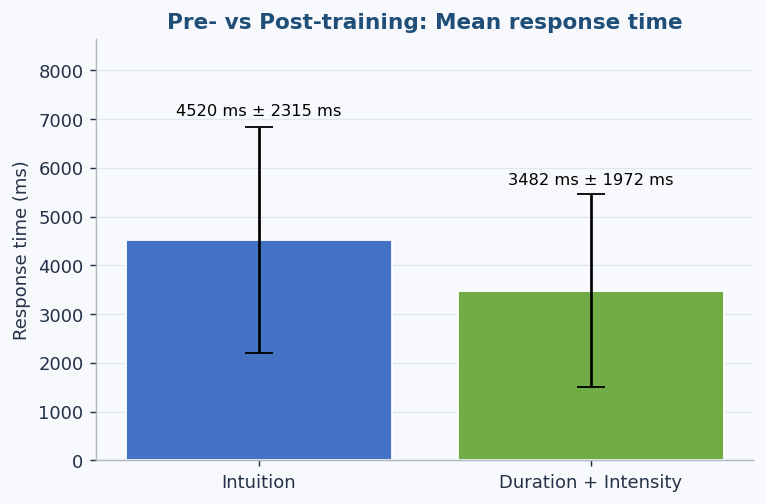
\includegraphics[width=0.8\linewidth]{training_effect_rt.png}
    \caption{Mean response times before and after training.}
    \label{fig:training_effect_rt}
\end{figure}

Training additionally improved response speed. As shown in Figure~\ref{fig:training_effect_rt}, the mean response time decreased from $4520 \pm 2315$ ms to $3482 \pm 1972$ ms, corresponding to a reduction of approximately 23.0\% ($p = 1.53 \times 10^{-5}$, $r = 0.73$). This decrease indicates that participants required less time to identify and classify the presented haptic signals once they had gained experience with the signal set.

Overall, the training procedure significantly improved participant performance across all measured dimensions. Following training, participants recognized signals more accurately, responded more quickly, and reported higher confidence levels. These findings demonstrate that the proposed haptic vocabulary can be learned effectively and that familiarity with the signals substantially enhances recognition performance.

\begin{figure}[H]
    \centering
    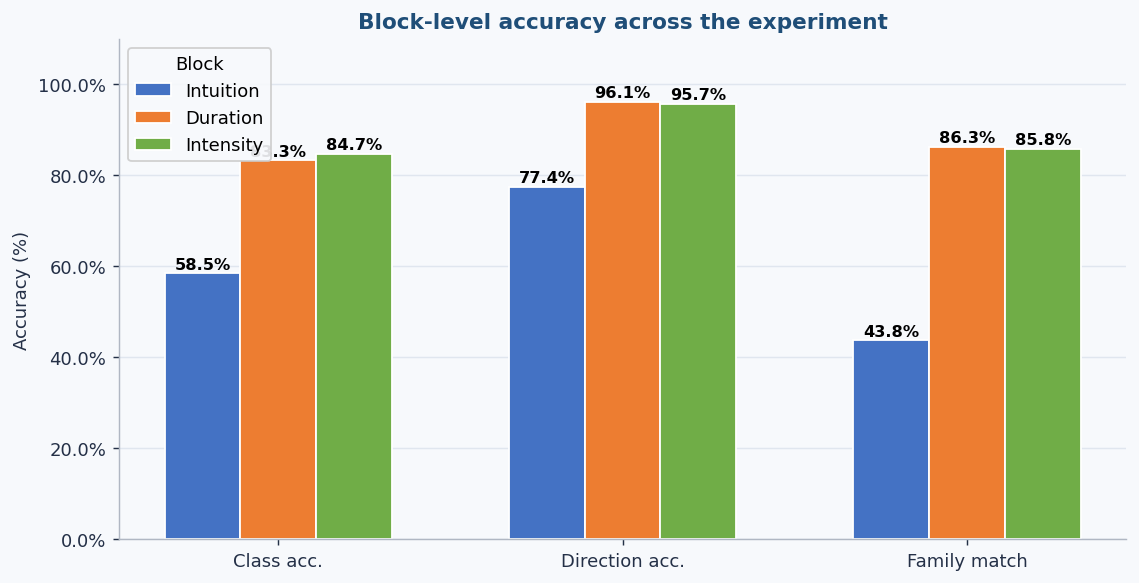
\includegraphics[width=0.5\linewidth]{all_blocks_accuracy_graph.png}
    \caption{Accuracy percentages across all blocks.}
    \label{fig:all_blocks_accuracy}
\end{figure}

\subsubsection*{Intuition Block Analysis}

\begin{figure}[!ht]
    \centering
    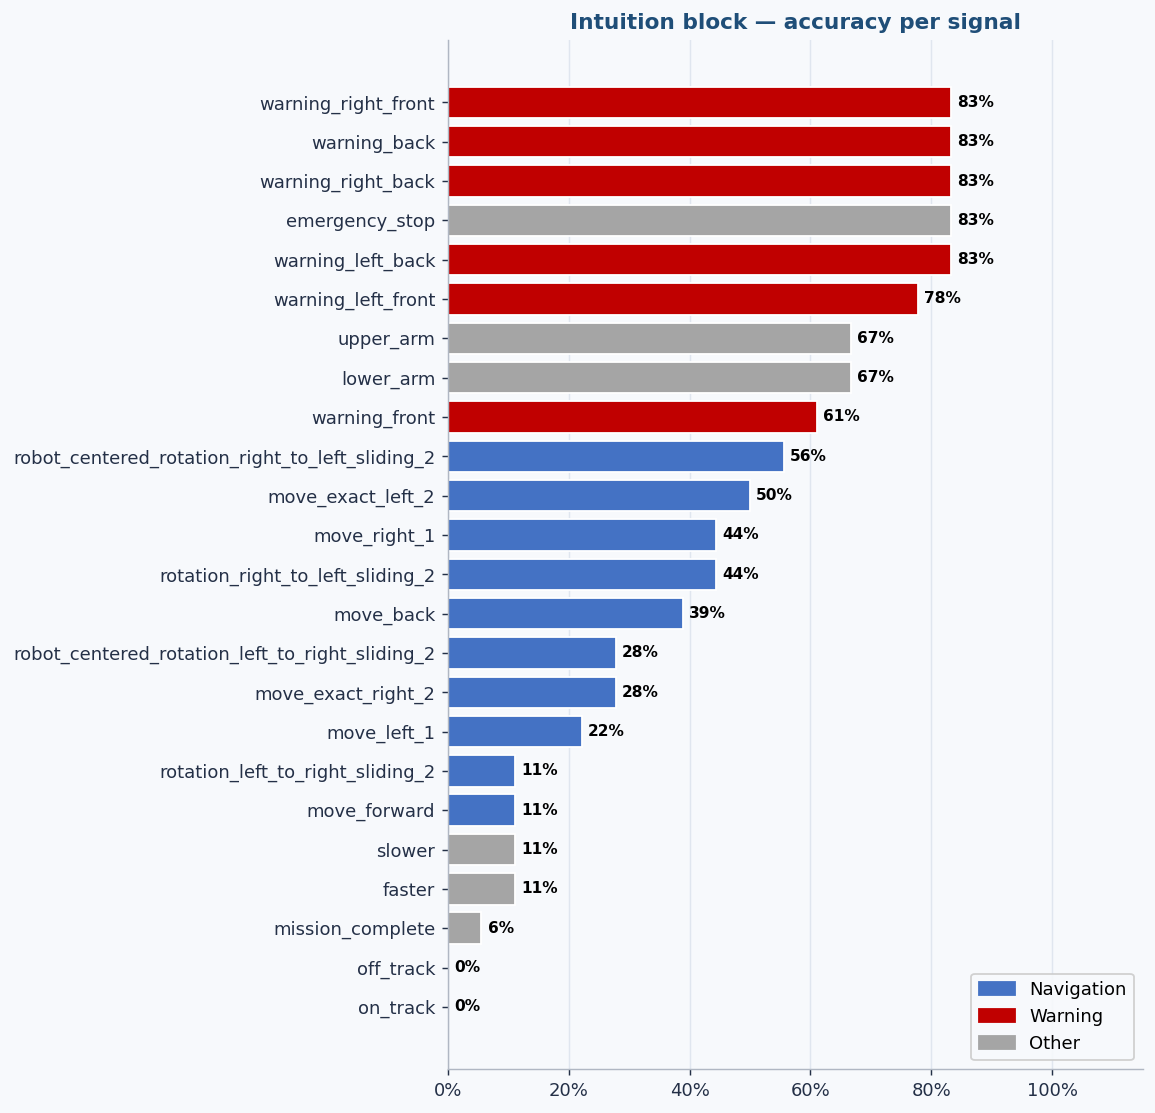
\includegraphics[width=0.8\linewidth]{intuition_signal_list.png}
    \caption{List of signals tested in the intuition block.}
    \label{fig:intuition_signal_list}
\end{figure}

To compare the intuitiveness of different signal categories, navigation and warning signals were analyzed separately using participant-level averages and Wilcoxon signed-rank tests. Warning signals consistently outperformed navigation signals across both recognition accuracy and response speed. Participants recognized warning signals significantly more accurately than navigation signals (78.7\% vs. 33.3\%, Wilcoxon signed-rank test, $p = 2.0 \times 10^{-4}$, $r = 0.878$). Similarly, warning signals were classified more accurately according to their signal category (82.2\% vs. 46.9\%, $p = 3.2 \times 10^{-4}$, $r = 0.847$). In addition, warning signals were recognized significantly faster, with mean response times of 3618 ms compared to 4618 ms for navigation signals ($p = 8.4 \times 10^{-4}$, $r = 0.734$).

\begin{figure}[H]
\centering
\begin{minipage}{0.49\textwidth}
    \centering
    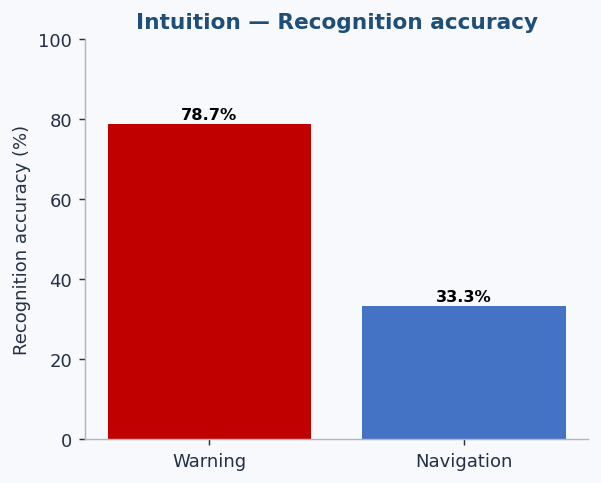
\includegraphics[width=\linewidth]{intuition_accuracy.png}
\end{minipage}
\hfill
\begin{minipage}{0.49\textwidth}
    \centering
    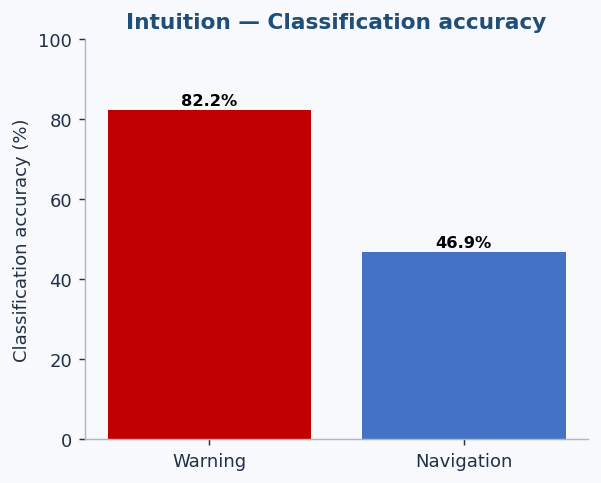
\includegraphics[width=\linewidth]{intuition_classification.png}
\end{minipage}
\caption{Mean recognition and classification accuracy levels in the intuition (pre-training) block.}
\label{fig:intuition_accuracy_class}
\end{figure}

A closer examination of navigation signal performance revealed that participants were often able to identify the general direction conveyed by the signal but struggled to distinguish the exact navigation command. While directional recognition accuracy reached 59.4\%, exact recognition accuracy remained substantially lower at 33.3\%. This finding suggests that many navigation signals were interpreted as generic directional or warning-like cues rather than as distinct navigation commands. Overall, the results indicate that warning signals were inherently more intuitive and easier to interpret, whereas navigation signals would benefit from further refinement to improve their distinctiveness and reduce ambiguity.

Movement modulation signals exhibited lower recognition performance than navigation and warning signals, which was expected since these signals are conveyed through distinct vibration patterns rather than intuitive directional cues. Unlike navigation and warning signals, whose meanings can often be inferred from the stimulated body location, movement modulation signals require participants to learn an arbitrary mapping between the vibration pattern and its intended meaning. Consequently, these signals were generally perceived as less intuitive.

Nevertheless, certain movement modulation signals achieved relatively high recognition rates. In particular, the \textit{Upper Arm} and \textit{Lower Arm} commands benefited from a natural correspondence between the vibration pattern and the intended action. Participants were able to associate the discrete upward and downward progression of the vibration with the corresponding direction of motion, making these signals easier to interpret. This observation suggests that incorporating spatial or motion-consistent metaphors into haptic signal design can improve intuitiveness and facilitate faster learning of more abstract commands.

\subsubsection*{Duration Level Based Analysis}

\begin{figure}[H]
    \centering
    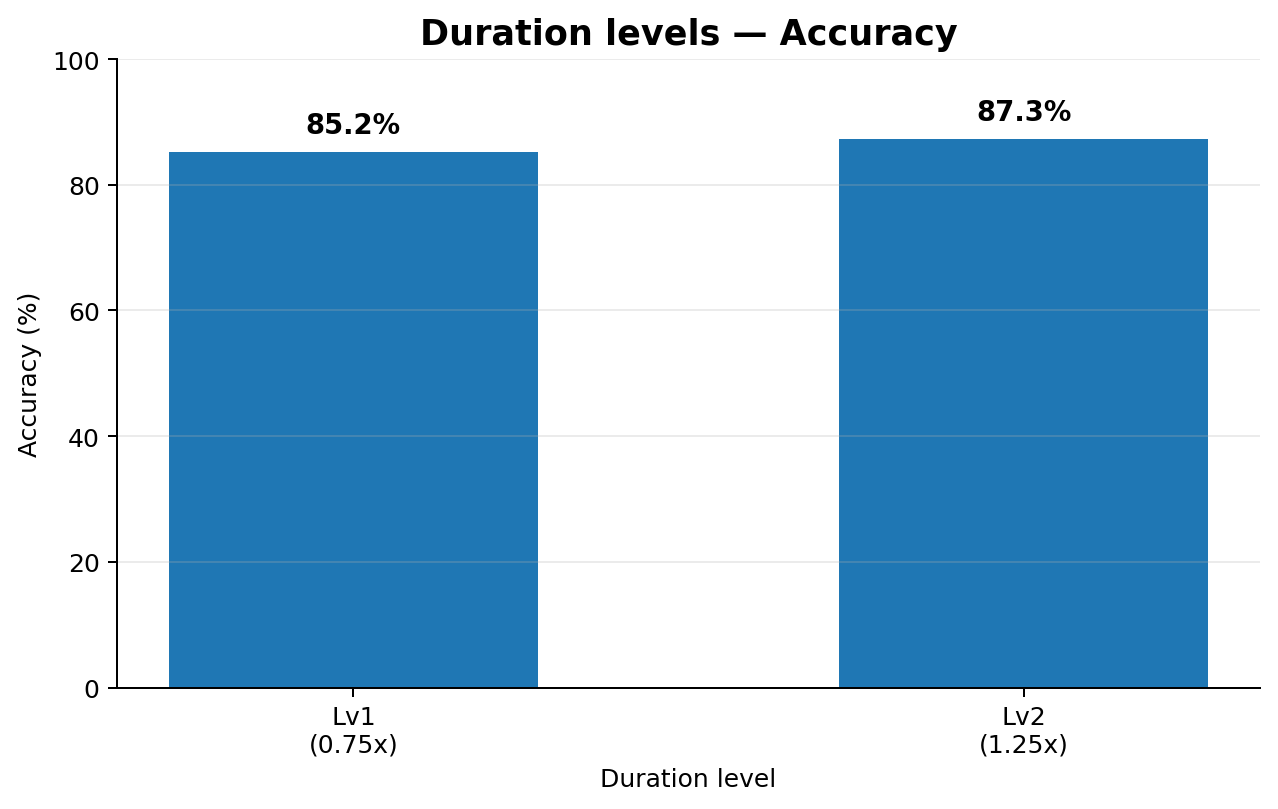
\includegraphics[width=0.5\linewidth]{duration_accuracy_mean.png}
    \caption{Mean accuracy percentages comparing the two duration levels.}
    \label{fig:duration_accuracy_mean}
\end{figure}

To evaluate the effect of signal duration, participant responses to the short-duration (Level 1) and long-duration (Level 2) variants of the same signals were compared using participant-level averages and Wilcoxon signed-rank tests. Increasing signal duration resulted in significantly longer response times, with the average response time increasing from 3372 ms to 3633 ms ($p = 0.0159$, $r = 0.559$). This result is expected, as participants generally waited for a larger portion of the signal before making a decision when longer stimuli were presented.

Although longer duration signals produced a modest increase in overall recognition accuracy (85.2\% to 87.3\%), this improvement was not statistically significant ($p = 0.201$). However, signal duration had a more pronounced effect on movement modulation signals. For this signal category, recognition accuracy increased significantly from 83.3\% to 90.3\% ($p = 0.0067$, $r = 0.891$), suggesting that the additional temporal information provided by longer patterns helped participants distinguish between more complex, non-directional vibration sequences.

\begin{figure}[H]
\centering
\begin{minipage}{0.49\textwidth}
    \centering
    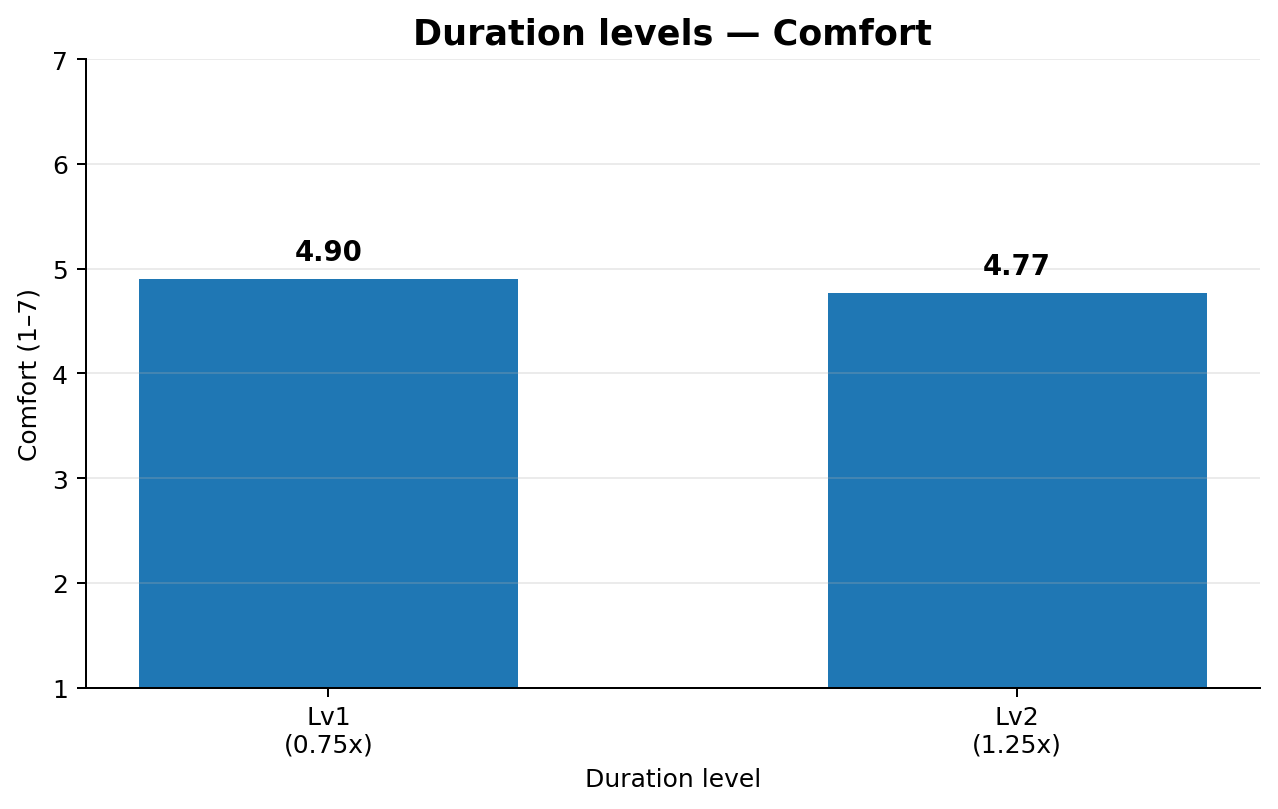
\includegraphics[width=\linewidth]{duration_comfort_mean.png}
\end{minipage}
\hfill
\begin{minipage}{0.49\textwidth}
    \centering
    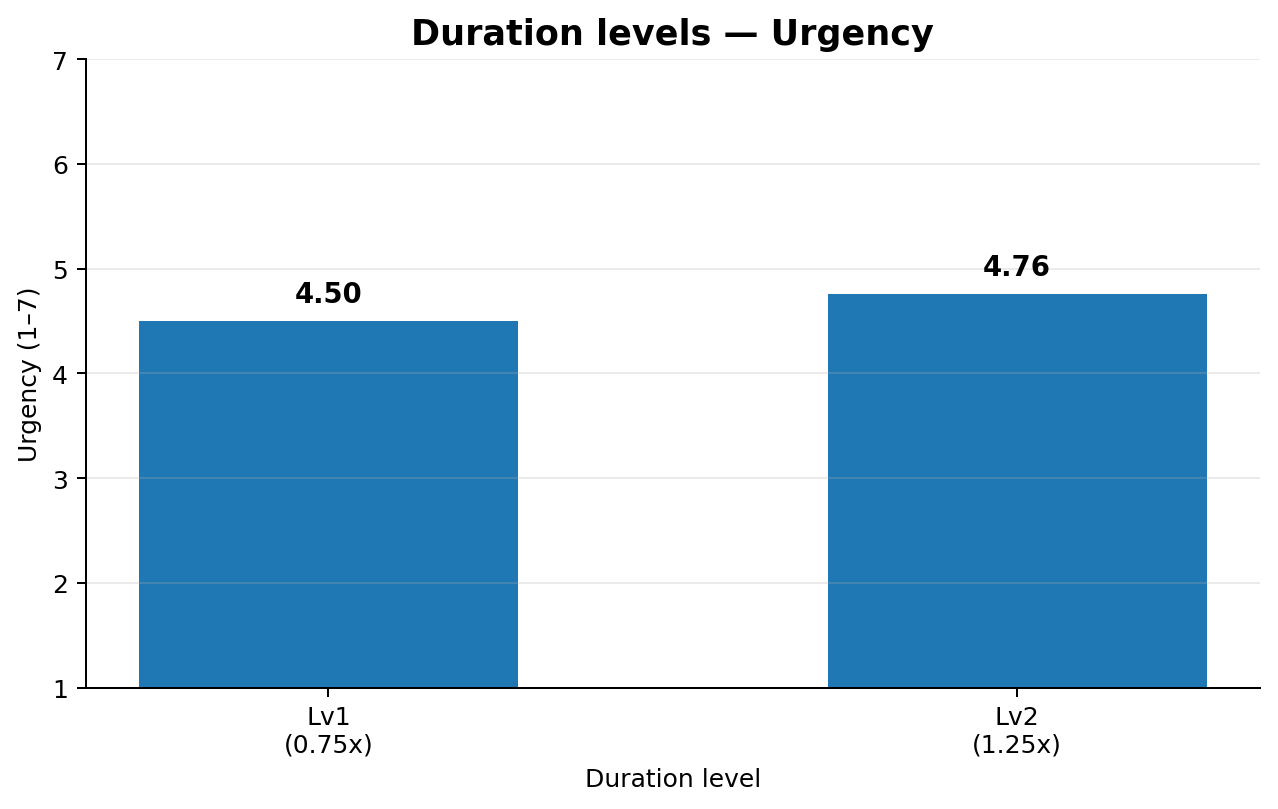
\includegraphics[width=\linewidth]{duration_urgency_mean.png}
\end{minipage}
\caption{Mean comfort and urgency ratings for the two duration levels.}
\label{fig:duration_comfort_urgency}
\end{figure}

Duration also influenced subjective perceptions of the signals. Longer duration signals were perceived as significantly more urgent ($p = 0.0048$, $r = 0.683$), with Level 2 signals consistently receiving higher urgency ratings across all signal classes. This finding indicates that signal duration itself contributes to the perception of urgency, independent of the signal content. Conversely, shorter duration signals were rated as significantly more comfortable, with mean comfort ratings decreasing from 4.9 to 4.77 for the longer-duration condition ($p = 0.041$, $r = 0.603$). This suggests a trade-off between urgency and user comfort when selecting signal duration parameters.

For warning signals, recognition performance remained extremely high at both duration levels (98.6\% and 91.7\%), indicating that these signals were highly robust to duration changes. Even though a small reduction in accuracy was observed for longer warning signals, participants were able to recognize them reliably regardless of duration. Overall, the results suggest that extending signal duration primarily affects response speed, urgency perception, and the recognition of more complex movement modulation signals, while providing limited benefit for already highly recognizable warning signals.

\subsubsection*{Intensity Level Based Analysis}

\begin{figure}[H]
\centering
\begin{minipage}{0.49\textwidth}
    \centering
    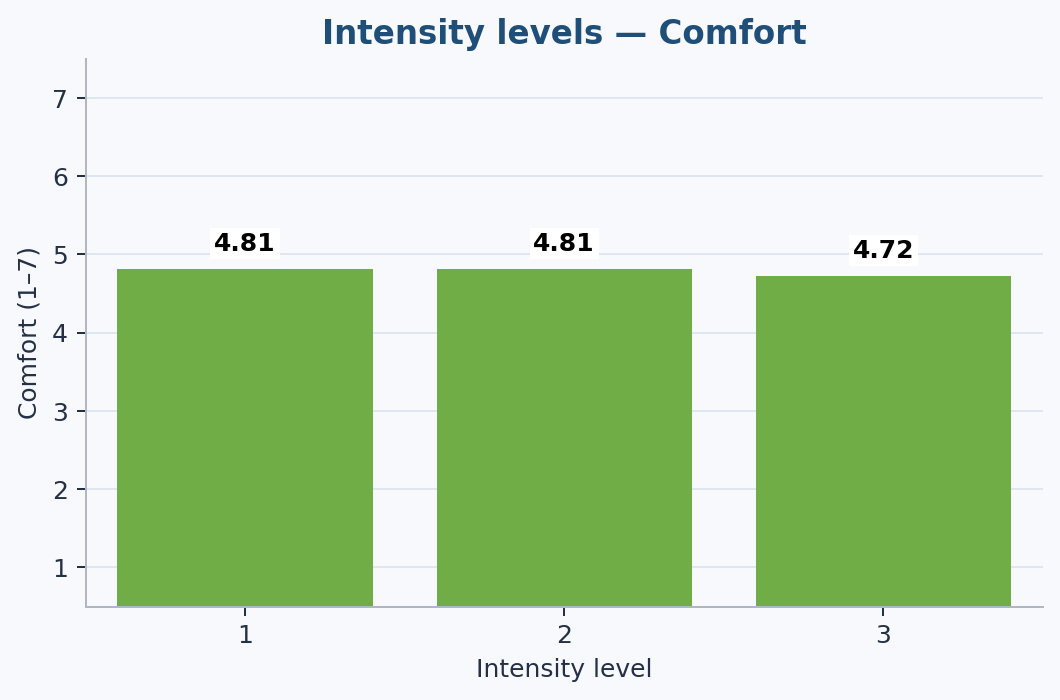
\includegraphics[width=\linewidth]{intensity_levels_comfort_mean_labels.png}
\end{minipage}
\hfill
\begin{minipage}{0.49\textwidth}
    \centering
    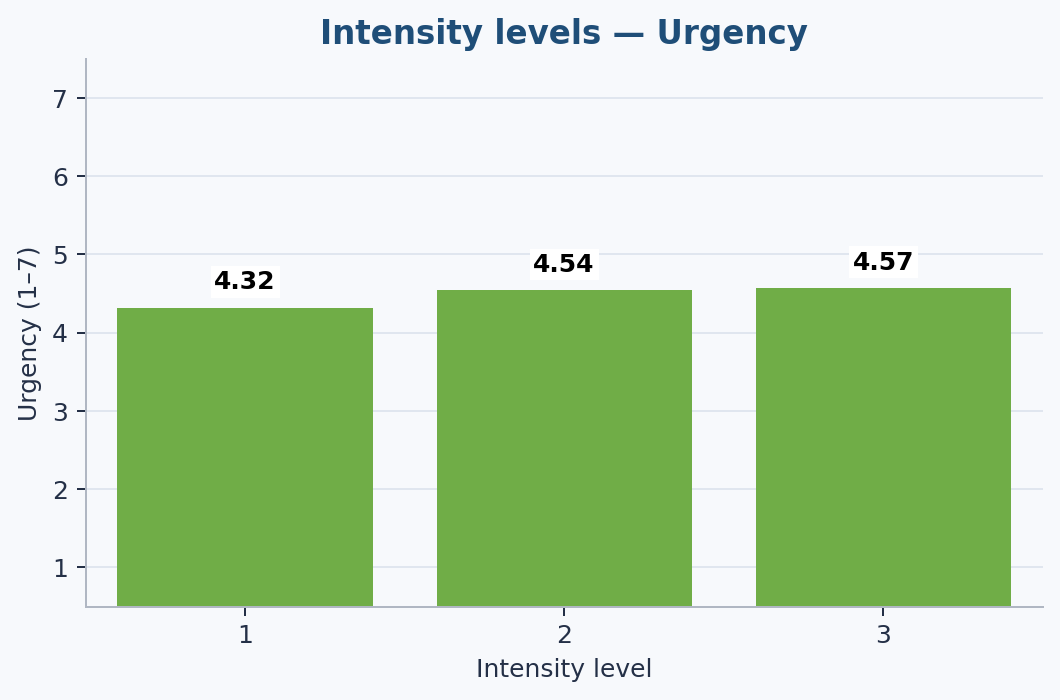
\includegraphics[width=\linewidth]{intensity_levels_urgency_mean_labels.png}
\end{minipage}
\caption{Mean comfort and urgency ratings for all three intensity levels.}
\label{fig:intensity_comfort_urgency}
\end{figure}

To evaluate the influence of vibration intensity, participant responses were compared across three intensity levels using participant-level averages. Since the measurements were repeated and normality could not be assumed, Friedman tests were used to assess statistical differences between intensity conditions.

Recognition performance remained highly stable across all intensity levels. Exact signal recognition accuracy was 86.1\%, 85.7\%, and 86.1\% for intensity levels 1, 2, and 3, respectively. The effect of intensity on recognition accuracy was not statistically significant (Friedman test, $\chi^2(2)=0.10$, $p=0.950$). Similarly, direction recognition remained consistently high across all intensity levels (97.2\%, 97.8\%, and 96.7\%), with no significant differences observed ($\chi^2(2)=0.21$, $p=0.902$). Class recognition accuracy showed a small decreasing trend (86.3\%, 85.3\%, and 84.9\%), but this effect did not reach statistical significance ($\chi^2(2)=5.41$, $p=0.067$).

Response times were also largely unaffected by intensity level. Mean response times were 3572 ms, 3368 ms, and 3467 ms for intensity levels 1, 2, and 3, respectively, with no statistically significant differences between conditions ($\chi^2(2)=1.00$, $p=0.607$).

Although intensity had little influence on objective recognition performance, it affected subjective user perception. Mean urgency ratings increased from 4.32 to 4.54 and 4.57 as intensity increased, indicating that stronger vibrations tended to be perceived as more urgent. However, this trend narrowly missed statistical significance ($\chi^2(2)=5.33$, $p=0.069$). Comfort ratings showed the opposite tendency, decreasing slightly from 4.81 to 4.72 as intensity increased, although this effect was not statistically significant ($\chi^2(2)=1.85$, $p=0.397$).

Overall, the results suggest that vibration intensity has a substantially weaker influence on signal interpretability than signal structure or duration. Recognition accuracy remained nearly constant across all intensity levels, indicating that participants primarily relied on the spatial and temporal characteristics of the vibration patterns rather than vibration strength when interpreting the signals. Consequently, intensity appears to be more suitable as a secondary parameter for modulating perceived urgency than as a primary mechanism for improving signal recognition performance.

The relatively weak effect of intensity may be partially explained by the limited separation between the selected intensity levels. While the three intensity levels were intentionally chosen to remain comfortable and clearly perceptible, the differences between them may not have been sufficiently large to produce substantial changes in recognition performance or subjective ratings. Future studies could investigate a wider intensity range to determine whether larger amplitude differences result in stronger effects on urgency perception and signal interpretability.

\begin{figure}[H]
\centering
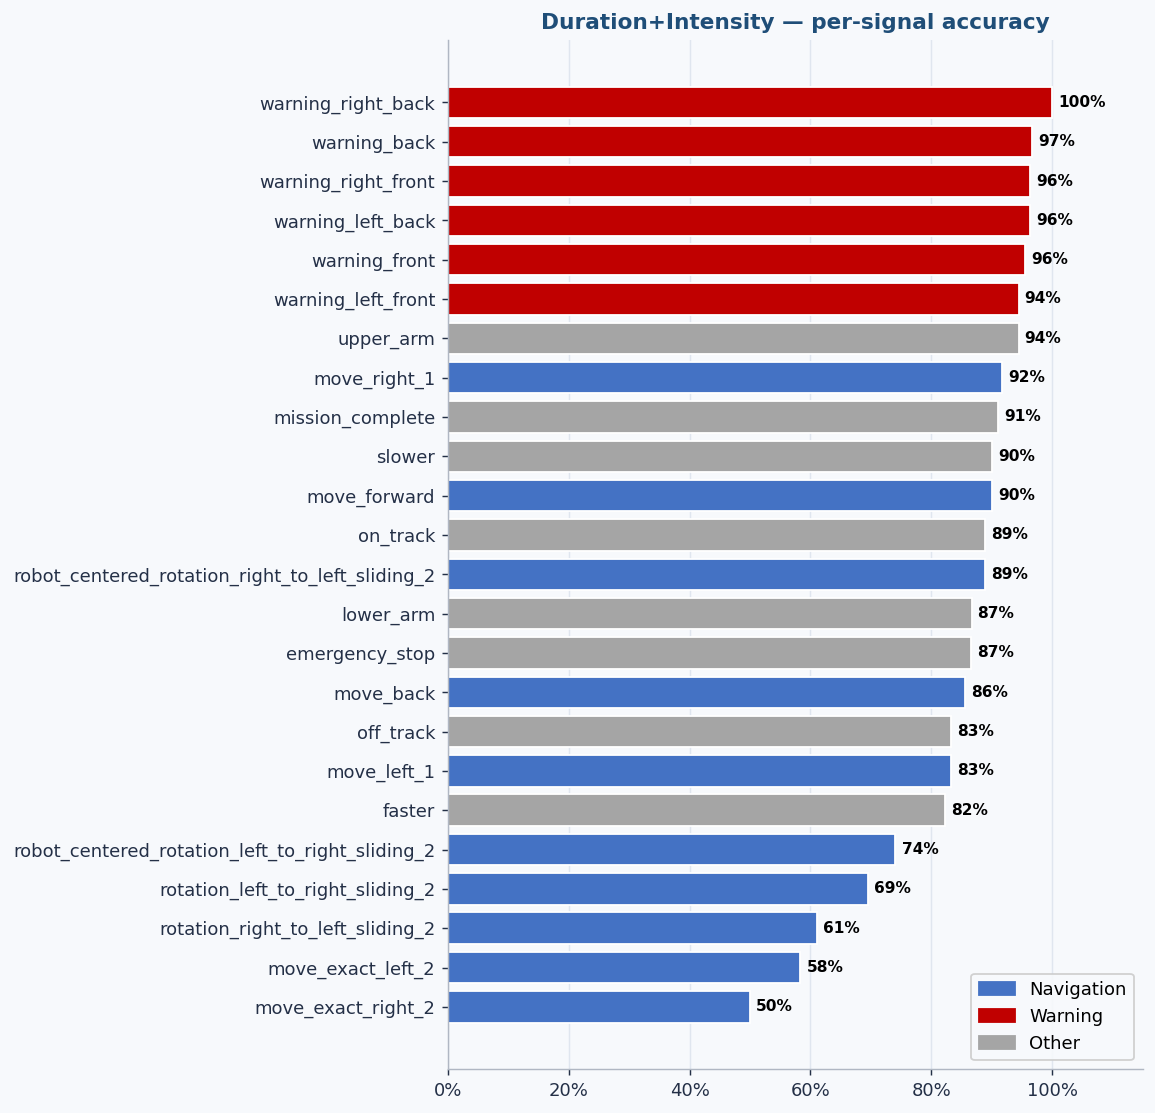
\includegraphics[width=0.85\linewidth]{per_signal_dur_int.png}
\caption{List of signals tested in the duration and intensity blocks combined.}
\label{fig:per_signal_dur_int}
\end{figure}

\subsubsection*{Accuracy Depending on Direction}

Direction-based accuracy showed a clear improvement after training. In the intuition block, participants recognized backward and left directions better than forward and right, with the lowest pre-training accuracy observed for forward signals at 36.1\% and right signals at 42.9\%. After training, all directions improved substantially in the duration block, reaching around 80.6--88.9\% accuracy. The intensity block showed the highest performance for forward and backward directions, with accuracies of 95.4\% and 92.6\%, respectively. However, left and especially right directions remained comparatively weaker in the intensity block, with right-direction accuracy decreasing to 73.5\%. Overall, these results suggest that training strongly improved directional interpretation, but directional cues were not equally robust across all directions; forward and backward cues became highly reliable, whereas lateral directions, particularly rightward cues, may require further refinement to reduce directional ambiguity.

\begin{figure}[H]
    \centering
    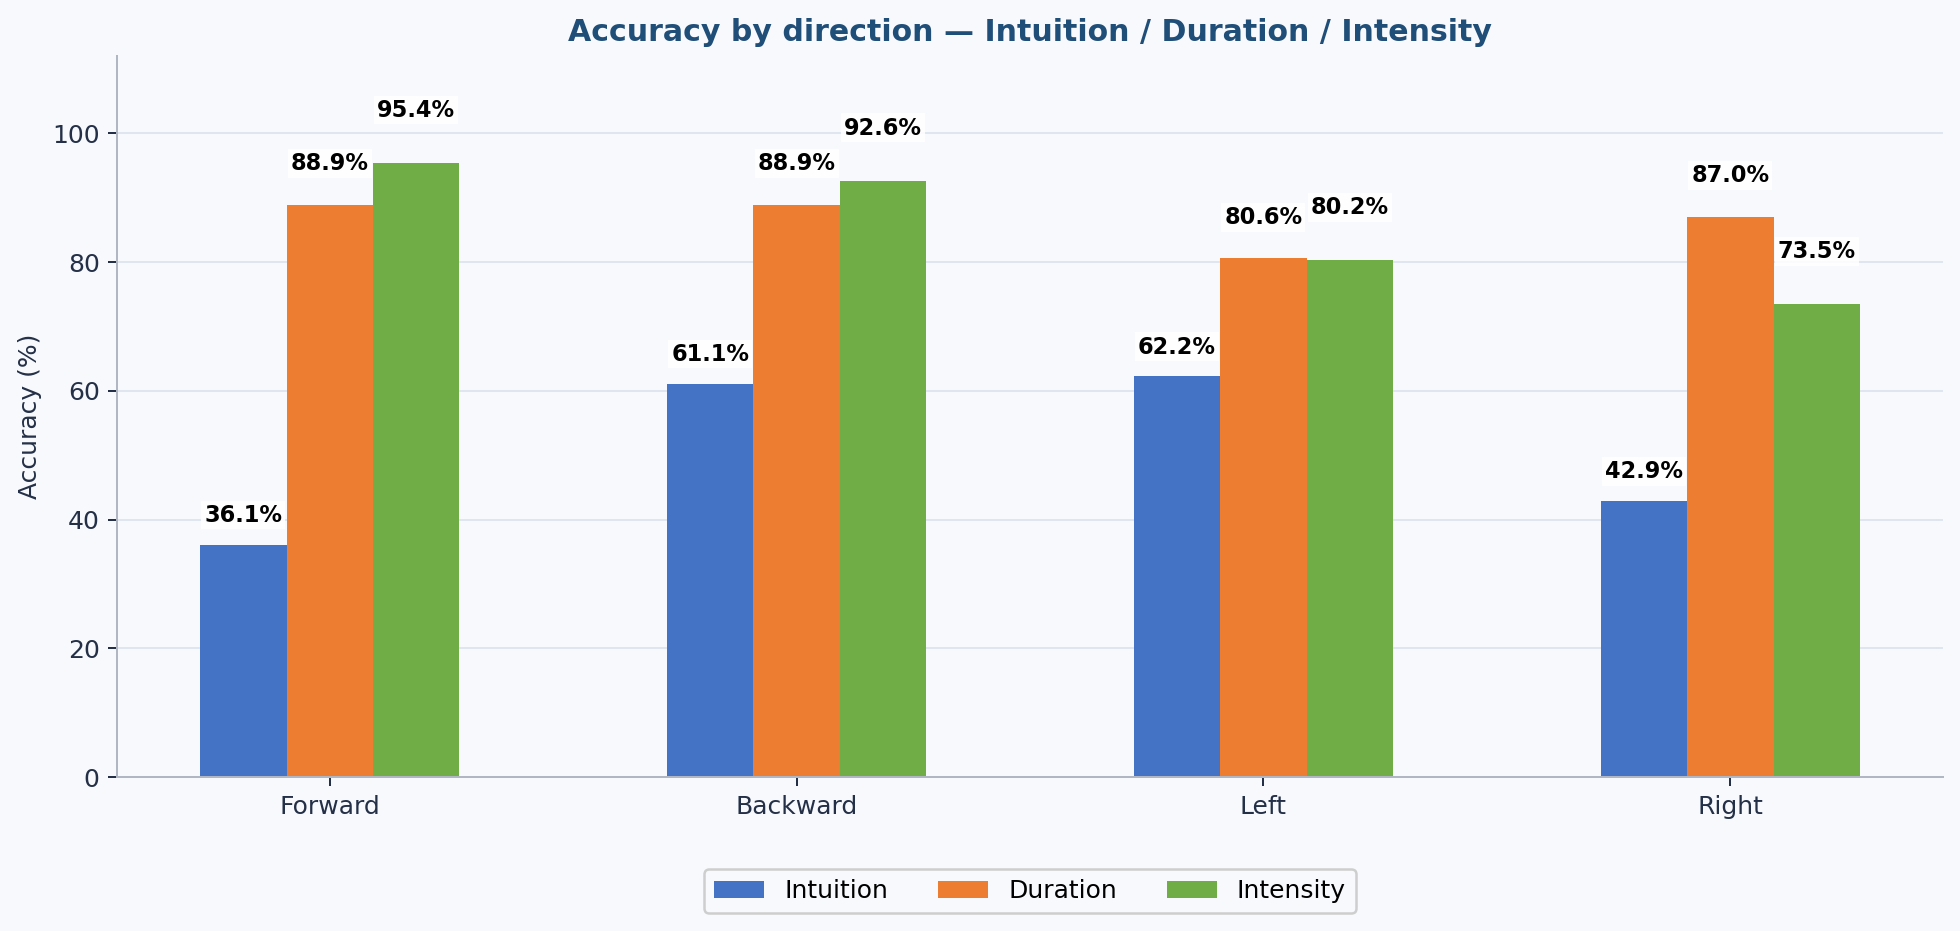
\includegraphics[width=1\linewidth]{direction_accuracy_mean_labels.png}
    \caption{Accuracy percentages for all directions.}
    \label{fig:direction_accuracy_mean}
\end{figure}

\begin{figure}[H]
    \centering
    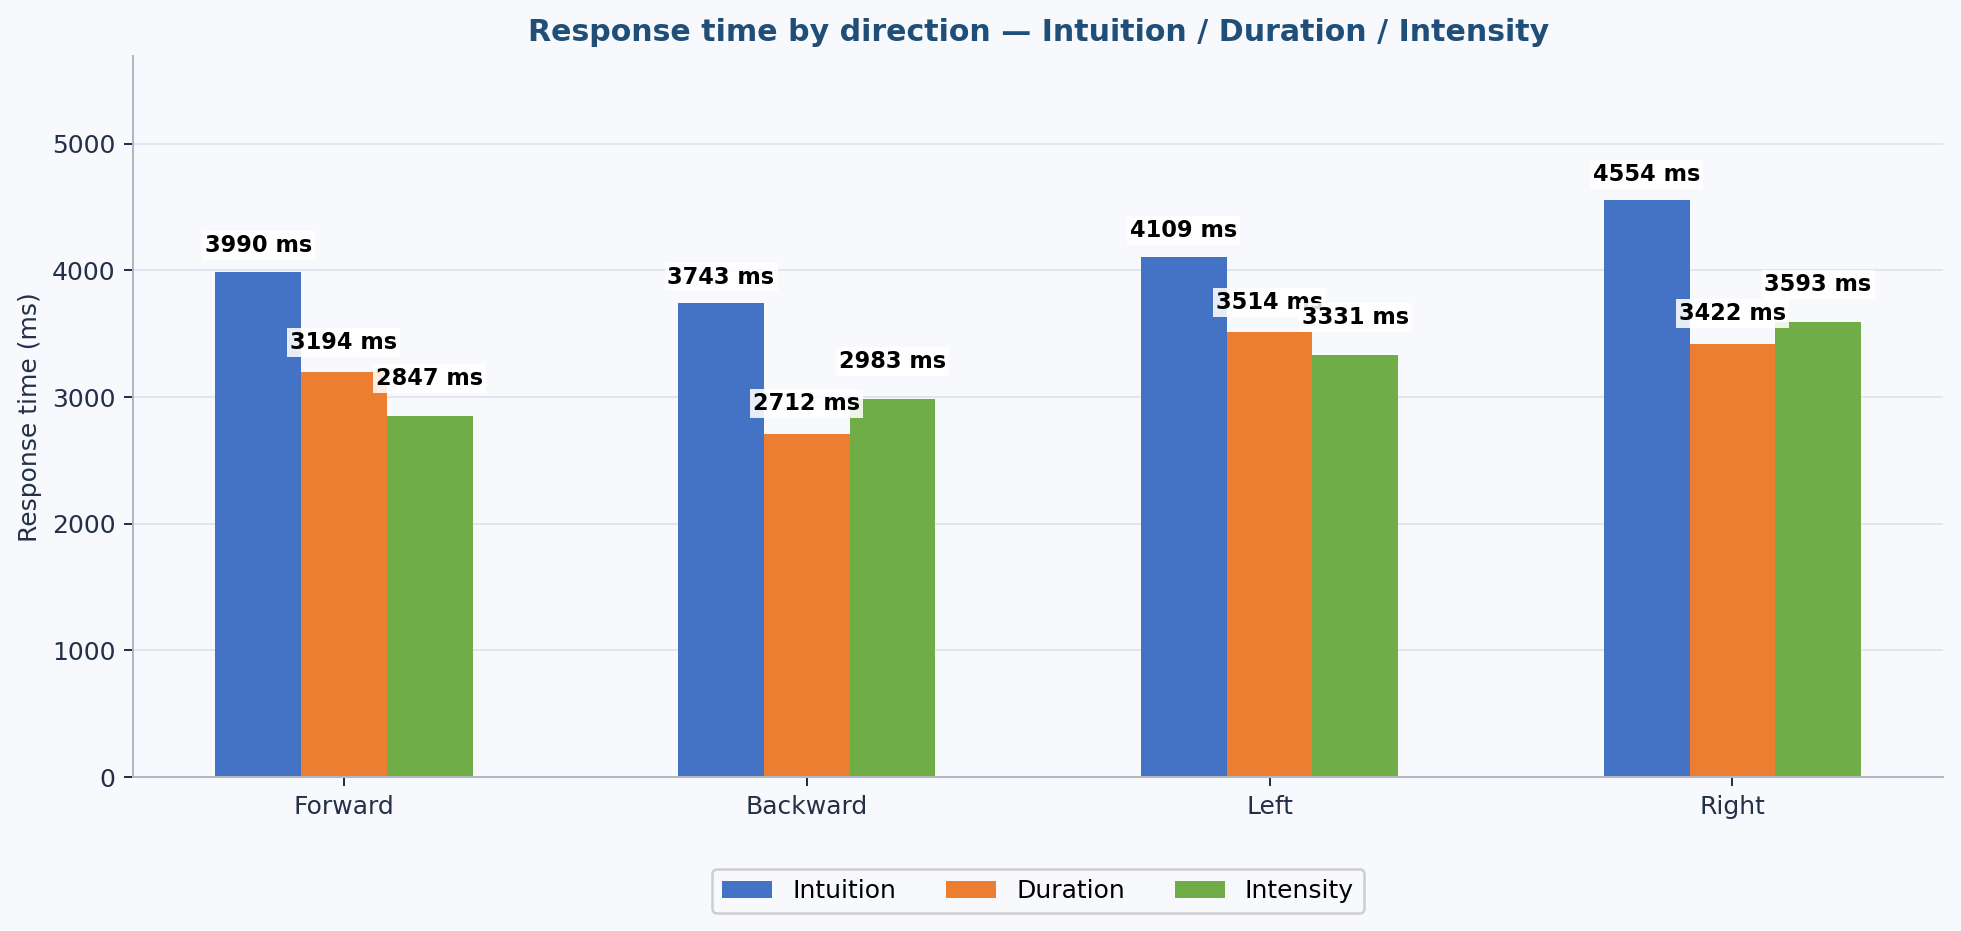
\includegraphics[width=1\linewidth]{direction_rt_mean_labels.png}
    \caption{Mean Response times for all directions.}
    \label{fig:direction_rt_mean_labels}
\end{figure}

\subsubsection*{Subjective Ratings}

In addition to objective performance measures such as accuracy and response time, participants evaluated each signal using three subjective metrics: confidence, comfort, and perceived urgency. Confidence reflects how certain participants were about their interpretation of the signal, comfort measures the perceived pleasantness of the haptic stimulation, and urgency represents the extent to which the signal conveyed an immediate need for action.

After each trial, participants were given the opportunity to provide optional written comments through the experimental interface. Furthermore, qualitative feedback was collected during the training phase and through discussions following the completion of the experiment. Throughout the design process, particular emphasis was placed on incorporating participant feedback, and several signal refinements were made based on observations and comments gathered during both the pilot and main studies.

Figures~\ref{fig:confidence_ratings}, \ref{fig:comfort_ratings}, and \ref{fig:urgency_ratings} summarize the average subjective ratings obtained in the intuition, duration, and intensity blocks. Error bars represent one standard deviation.

\begin{figure}[H]
    \centering
    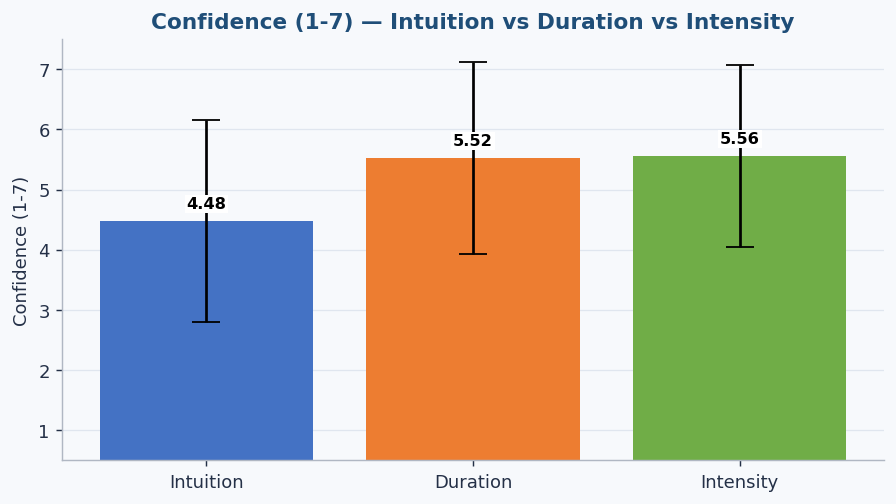
\includegraphics[width=0.5\linewidth]{confidence_ratings.png}
    \caption{Mean confidence ratings for all blocks.}
    \label{fig:confidence_ratings}
\end{figure}

As shown in Figure~\ref{fig:confidence_ratings}, confidence ratings increased substantially after training. Participants reported an average confidence of 4.48 during the intuition block, which increased to 5.52 and 5.56 in the duration and intensity blocks, respectively. This trend is consistent with the objective performance measures and suggests that participants became more familiar with the haptic vocabulary as the experiment progressed.

\begin{figure}[H]
    \centering
    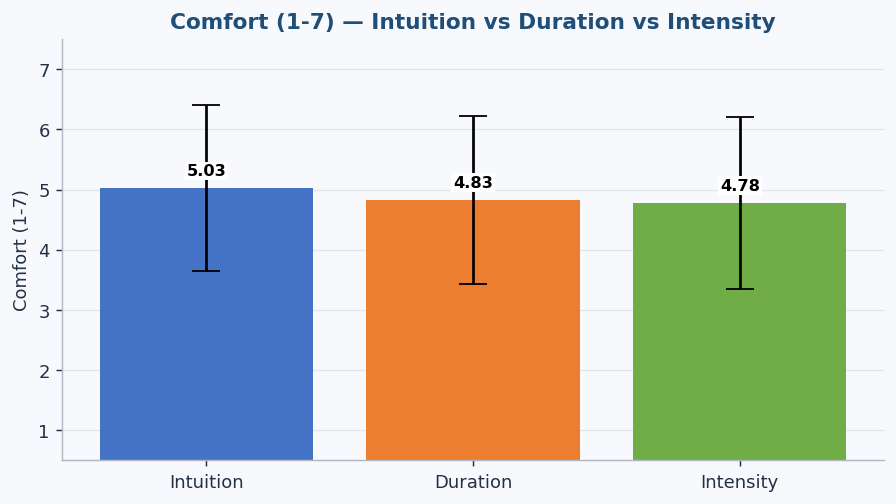
\includegraphics[width=0.5\linewidth]{comfort_ratings.png}
    \caption{Mean comfort ratings for all blocks.}
    \label{fig:comfort_ratings}
\end{figure}

Comfort ratings remained relatively stable across all experimental blocks (Figure~\ref{fig:comfort_ratings}). Mean comfort scores ranged between 4.78 and 5.03 on the seven-point scale, indicating that the majority of signals were perceived as moderately comfortable. The absence of a notable decrease in comfort despite prolonged exposure suggests that neither the signal duration nor the intensity manipulations introduced substantial discomfort.

\begin{figure}[H]
    \centering
    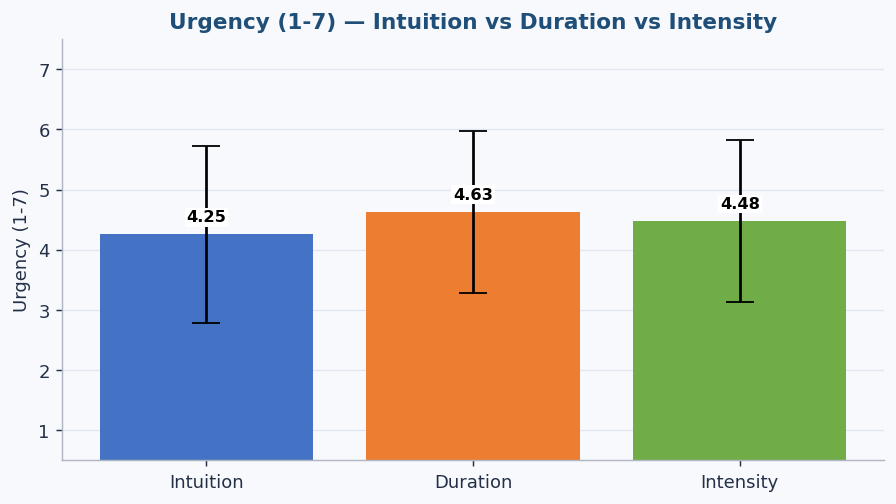
\includegraphics[width=0.5\linewidth]{urgency_ratings.png}
    \caption{Mean urgency ratings for all blocks.}
    \label{fig:urgency_ratings}
\end{figure}

Perceived urgency ratings exhibited a slight increase following training (Figure~\ref{fig:urgency_ratings}). The average urgency score increased from 4.25 in the intuition block to 4.63 and 4.48 in the duration and intensity blocks, respectively. This finding indicates that participants were better able to associate specific signals with their intended level of urgency after becoming familiar with the signal set.

To further investigate the effect of actuator location, subjective comfort and recognition accuracy were analyzed separately for front and back vest actuators and across gender groups. Figure~\ref{fig:front_back_gender} presents these results.

\begin{figure}[H]
\centering
\begin{minipage}{0.49\textwidth}
    \centering
    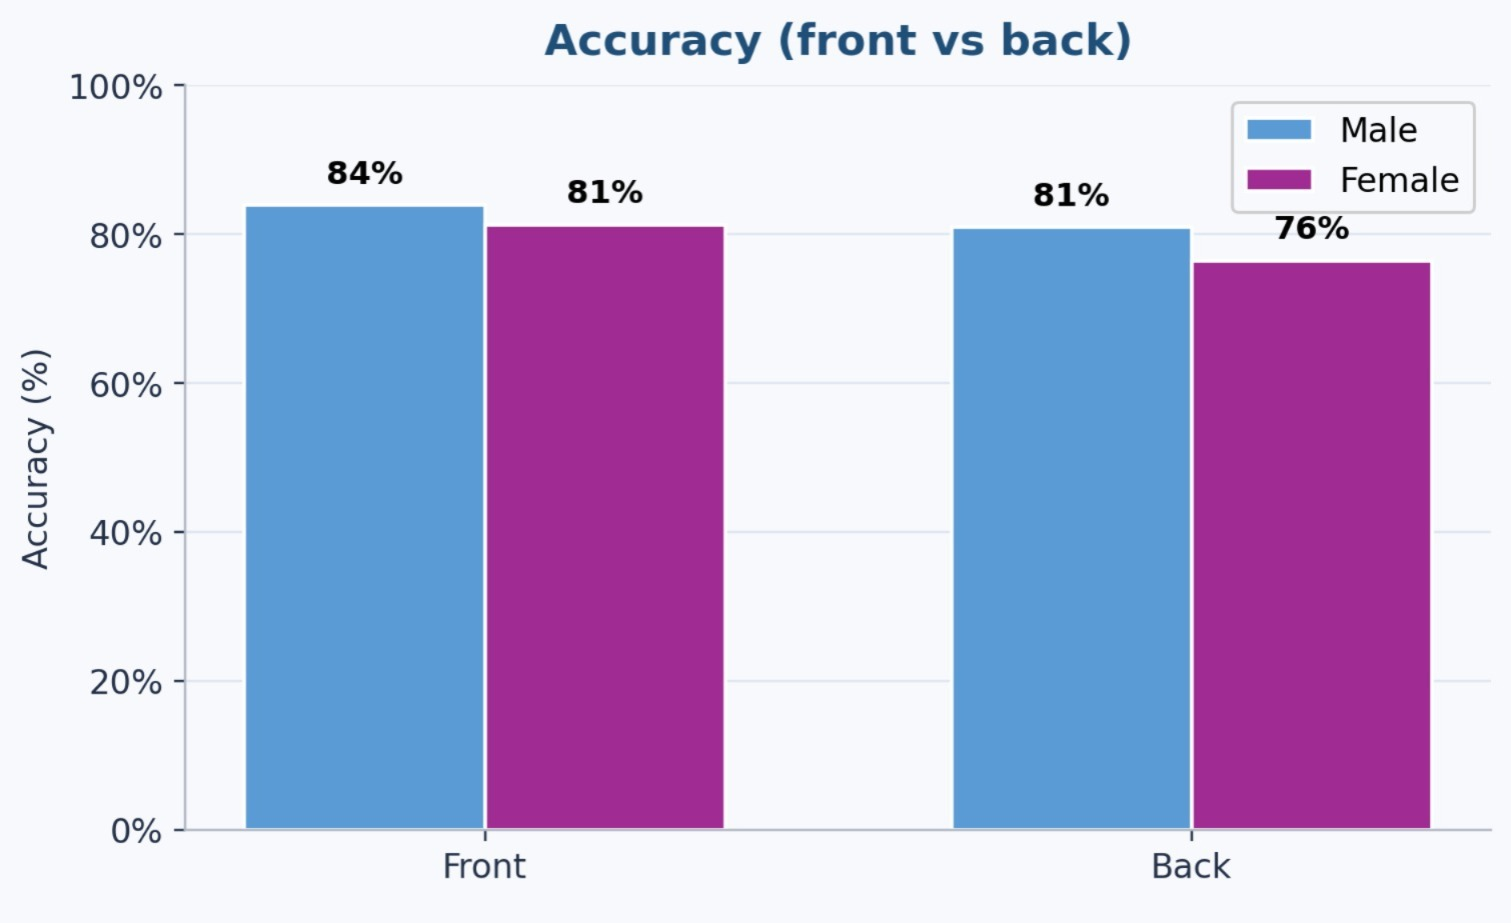
\includegraphics[width=\linewidth]{frontvsback_gender.jpeg}
\end{minipage}
\hfill
\begin{minipage}{0.49\textwidth}
    \centering
    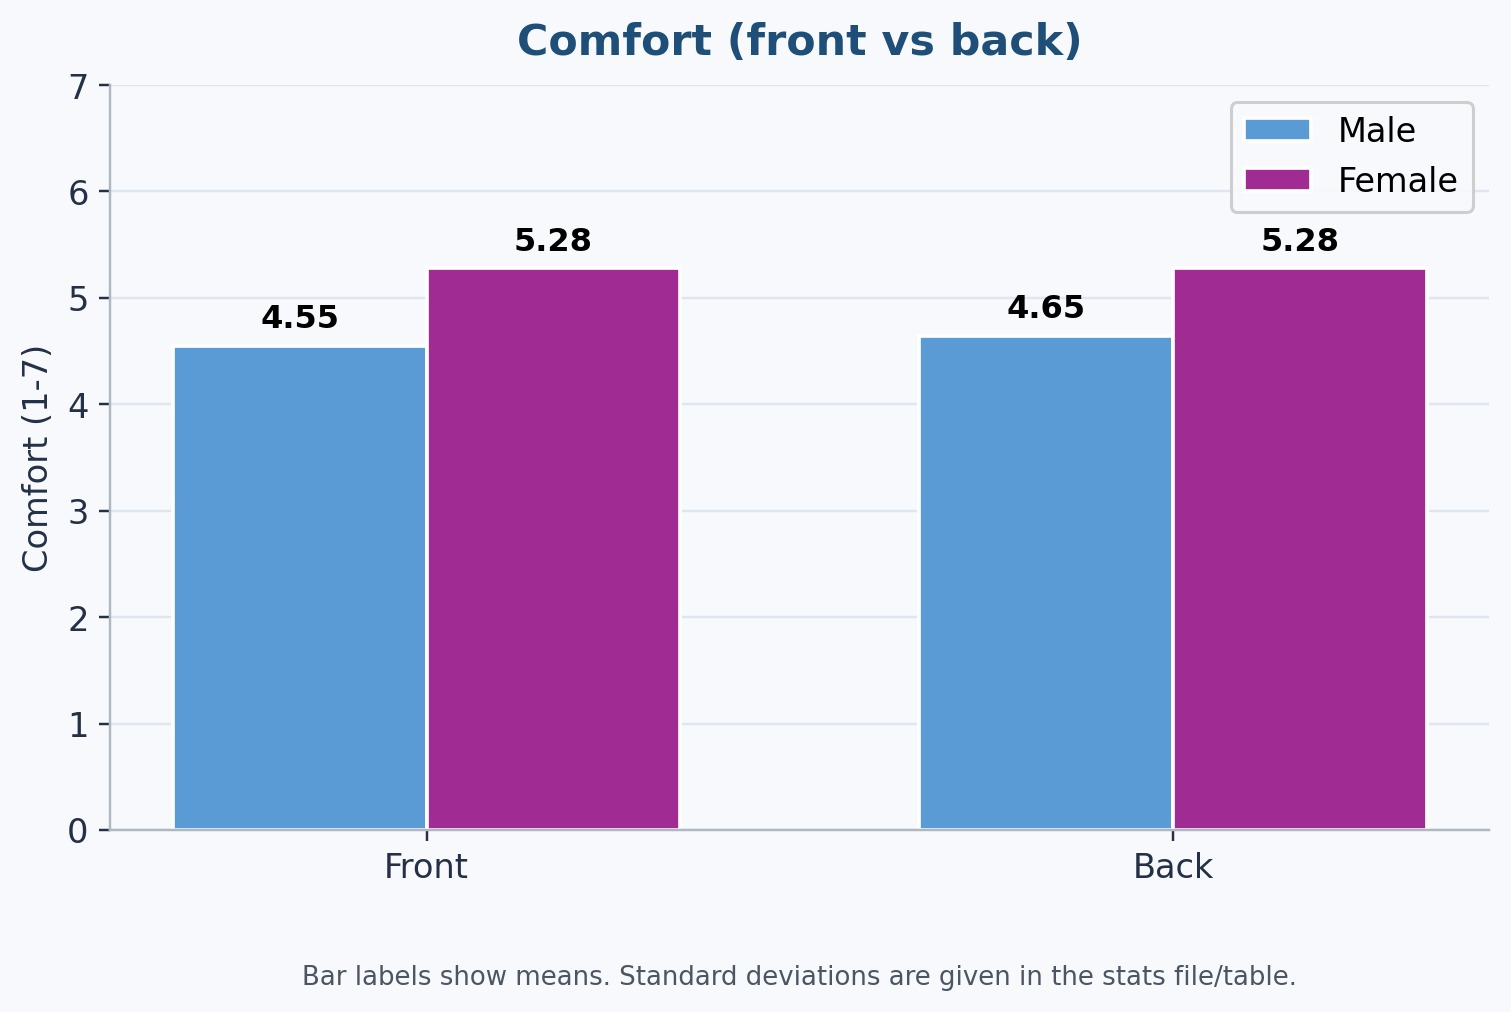
\includegraphics[width=\linewidth]{frontback_comfort_gender.jpeg}
\end{minipage}
\caption{Mean accuracy and comfort levels for front and back signals.}
\label{fig:front_back_gender}
\end{figure}

Female participants reported higher comfort ratings than male participants for both front and back actuator locations. While female participants rated front and back stimulation similarly, male participants showed a slight preference for signals actuated with back-mounted actuators. Despite these observable differences, Mann--Whitney U tests did not reveal a statistically significant effect of gender on comfort ratings ($p=0.146$). Similar non-significant results were obtained for confidence ($p=0.122$), response time ($p=0.203$), and recognition accuracy ($p=0.594$).

Signal recognition accuracy was generally comparable between front and back actuator locations. Male participants achieved average accuracies of approximately 84\% and 81\% for front and back signals, respectively, while female participants achieved average accuracies of approximately 81\% and 76\%. These results suggest that both front and back stimulation locations can effectively convey information, although a slight performance advantage was observed for front-mounted actuators.

Overall, the observed differences between gender groups and actuator locations were relatively small and did not reach statistical significance. This suggests that the proposed haptic vocabulary can be interpreted reliably across different user groups and stimulation locations.

The absence of statistically significant gender effects is encouraging from a design perspective, as it indicates that the haptic signals can be understood reliably across different user groups. Nevertheless, the consistently higher comfort ratings reported by female participants may warrant further investigation in future studies involving larger participant populations.

Overall, the subjective ratings indicate that the proposed haptic signal set was generally well accepted by participants. Training increased participant confidence without negatively affecting comfort, while urgency ratings remained consistent with the intended purpose of the signals. Combined with the objective performance measures, these findings support the suitability of the selected signal set for use in the navigation system developed in Phase 2.

\subsubsection*{Overview of Signal Scores}

\begin{figure}[H]
    \centering
    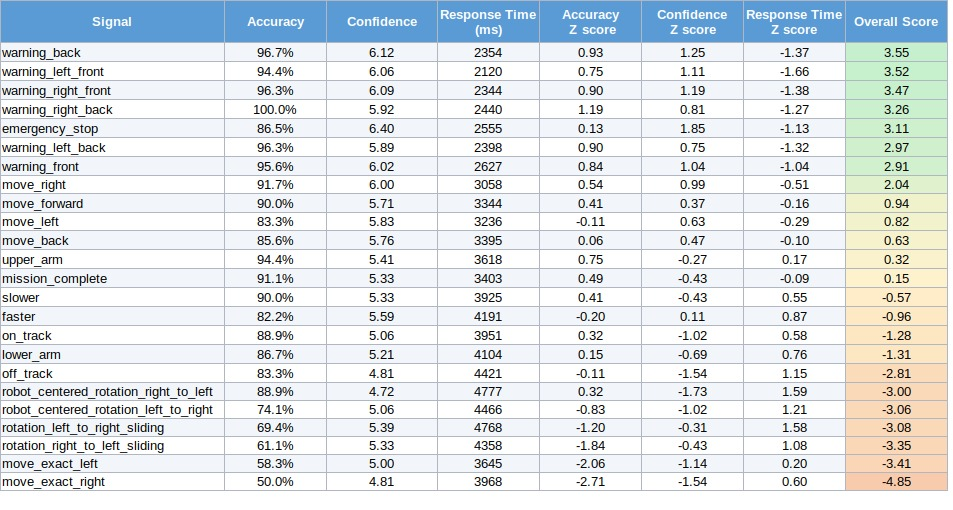
\includegraphics[width=1\linewidth]{overall_scores.jpeg}
    \caption{Overall Signal Scores.}
    \label{fig:overall_scores}
\end{figure}

To compare the overall effectiveness of the haptic signals, a composite score was computed using the standardized accuracy, confidence, and response time values:
\[
\text{Score} = z(\text{Accuracy}) + z(\text{Confidence}) - z(\text{Response Time})
\]

This metric rewards signals that are recognized accurately, interpreted with high confidence, and identified quickly. By combining these three dimensions into a single score, it becomes possible to evaluate the overall quality of each signal rather than focusing on a single performance metric. Higher scores therefore indicate stronger signal candidates for inclusion in the final haptic signal library.

The results show that warning signals consistently achieved the highest overall scores. Signals such as warning back, warning left front, warning right front, and warning right back occupied the top positions in the ranking, exhibiting high recognition accuracy, high confidence ratings, and relatively short response times. This outcome is particularly desirable from a safety perspective, as warning signals are intended to communicate urgent information, such as an approaching obstacle, that must be recognized quickly and reliably by a blind walker. The strong performance of these signals suggests that participants were able to distinguish and interpret safety-critical cues effectively.

In contrast, signals involving precise left-right directional discrimination achieved the lowest scores. In particular, move exact left, move exact right, and the rotational sliding signals showed lower accuracy, lower confidence, and longer response times compared to most other signals. These findings indicate that participants experienced greater difficulty distinguishing between fine-grained directional cues, suggesting that these patterns may benefit from further refinement. The overall signal ranking represents one of the most important outcomes of Phase 1, as it directly informed the final signal selection and design decisions. Rather than evaluating signals solely on intuition or individual metrics, the composite score provided an objective basis for identifying the most effective signal candidates and determining which patterns required redesign before integration into the path-tracking system developed in Phase 2.

\begin{figure}[H]
    \centering
    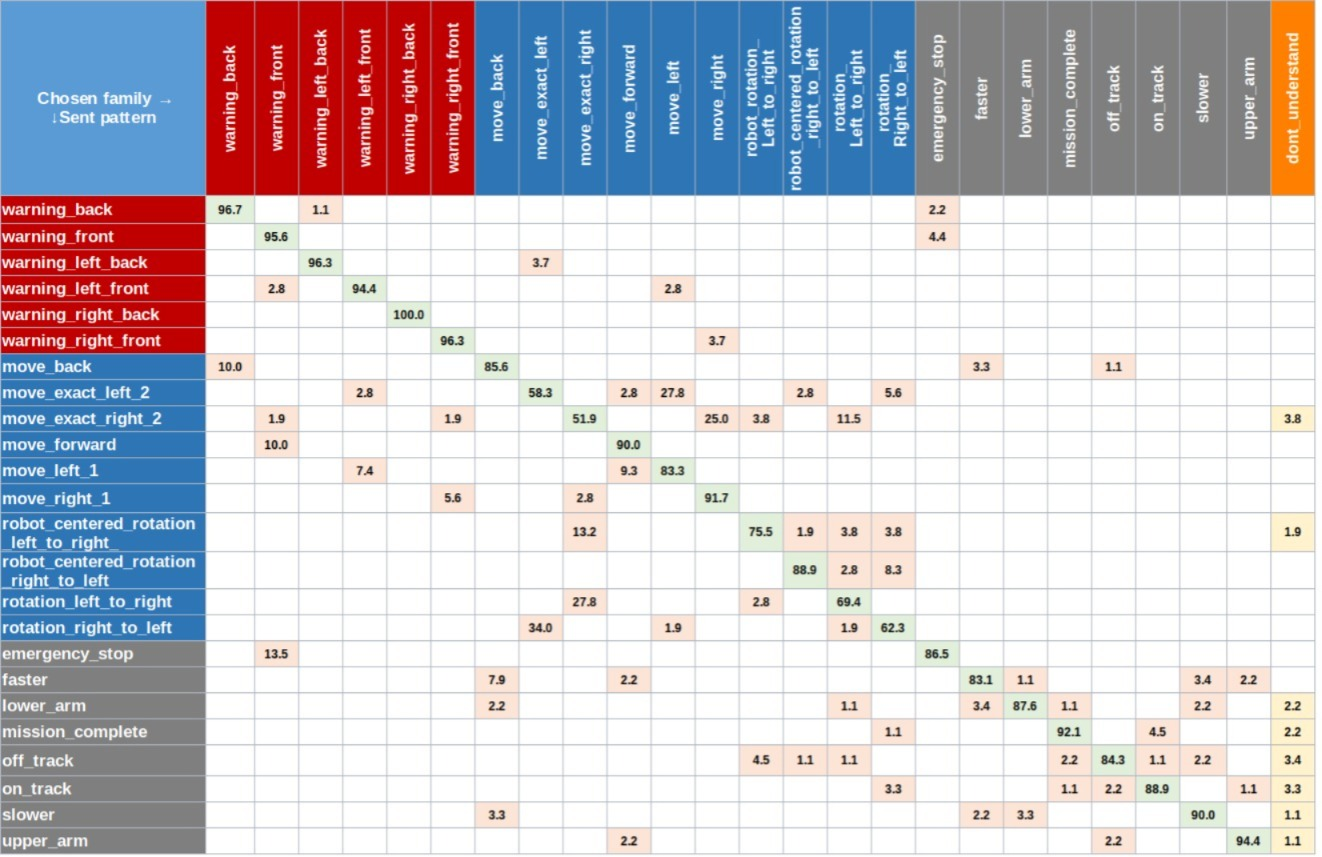
\includegraphics[width=1\linewidth]{combined_confusion_matrice.jpeg}
    \caption{Confusion Matrix for the signals in intensity + duration blocks combined.}
    \label{fig:combined_confusion_matrice}
\end{figure}

The confusion matrices served as one of the primary design evaluation tools throughout the study. While overall accuracy provides a single performance metric, confusion matrices reveal which specific signals are mistaken for each other and, therefore, provide direct insight into the intuitiveness of individual signal designs. Consequently, they were used extensively when refining the signal library and selecting the final signals for the Phase 2 navigation experiments.

\begin{figure}[H]
    \centering
    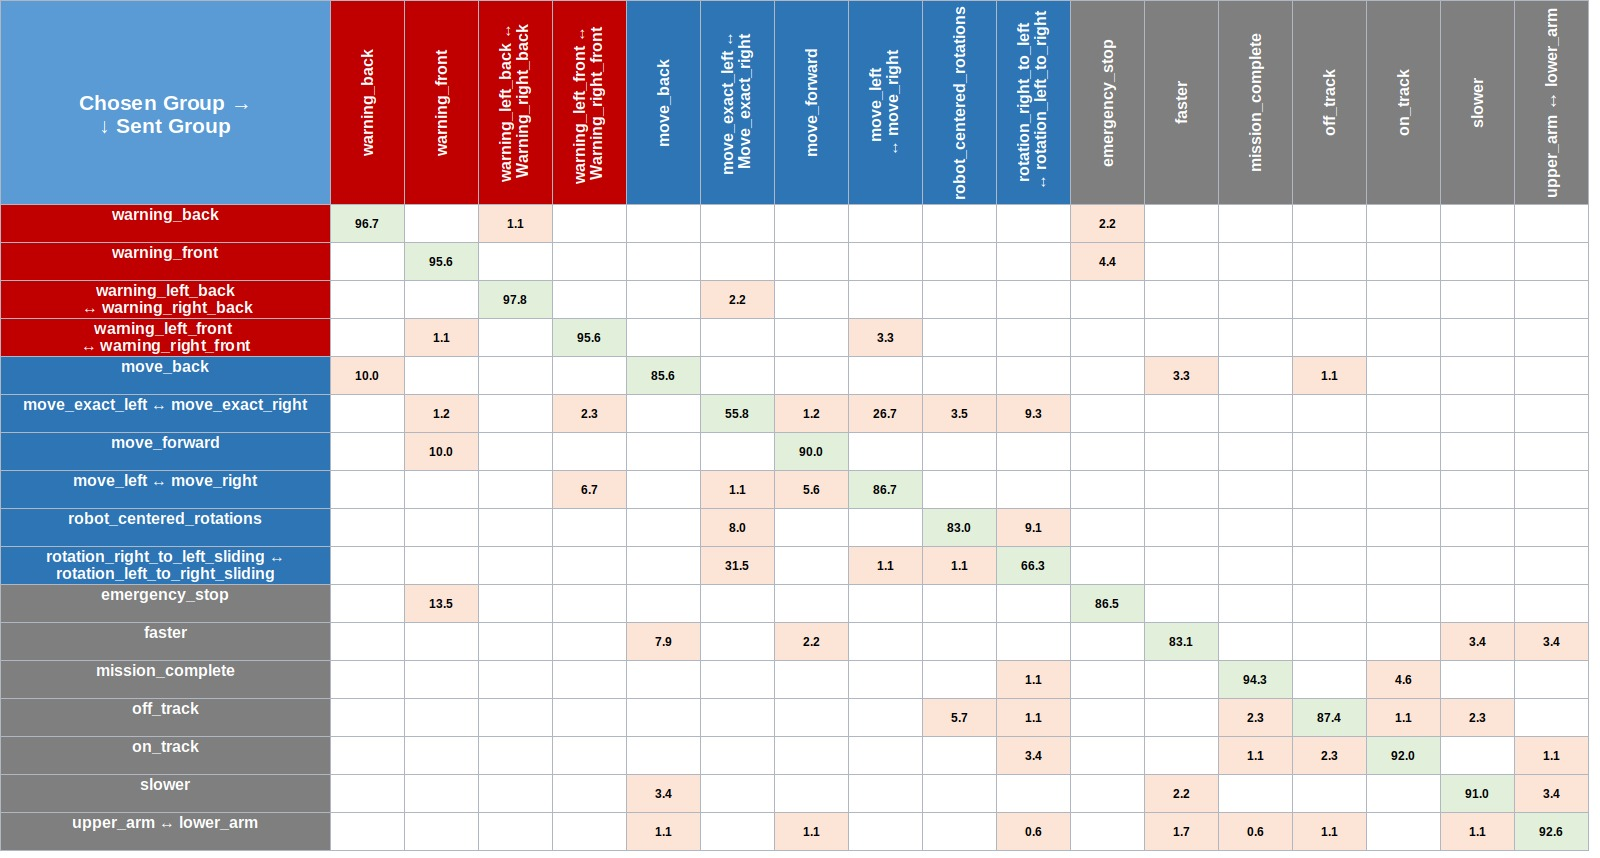
\includegraphics[width=1\linewidth]{symmetric_signals_confusion_matrix.jpeg}
    \caption{Confusion Matrix with symmetric signals merged in intensity + duration blocks.}
    \label{fig:symmetric_signals_confusion_matrix}
\end{figure}

Confusion matrices were generated for each experimental block individually, as well as for a combined dataset containing all post-training responses. In addition, a symmetric confusion matrix (Figure~\ref{fig:symmetric_signals_confusion_matrix}) was constructed by grouping left--right symmetric signals into common categories. This representation emphasizes conceptual recognition performance by removing errors arising solely from left--right inversions and highlighting broader signal interpretation patterns.

The matrices indicate that warning signals achieved consistently high recognition rates with very limited confusion, supporting their suitability for safety-critical notifications. In contrast, most confusion occurred among navigation signals that shared similar directional meanings. In particular, participants frequently confused exact directional cues with their corresponding coarse directional variants (e.g., \textit{Move Exact Left} and \textit{Move Left}) and occasionally confused rotational navigation cues with directional navigation cues representing the same turning direction. These observations motivated the redesign and removal of several low-performing navigation patterns and directly influenced the final signal selection used in Phase 2.

\subsection{Discussion and Future Work}

\subsubsection{Discussion}

This work presented a vibrotactile haptic vest framework for indoor navigation assistance for blind users. The two-phase experimental design allowed us to systematically evaluate both the interpretability of individual haptic signals and their applicability in navigation tasks.

The results of Phase 1 demonstrated that participants were able to learn and correctly interpret the proposed haptic signal vocabulary with high accuracy following a brief training session. Warning signals proved to be the most intuitive and reliably recognized category, achieving consistently high recognition rates even before training. Navigation signals, while initially more ambiguous, showed substantial improvement after training, indicating that the proposed signal designs are learnable and suitable for guiding users. Movement modulation signals, which rely on learned mappings rather than spatial metaphors, benefited most from training and from longer signal durations, suggesting that their design may require further refinement to improve pre-training intuitiveness. It should be noted that these results were obtained with sighted participants; whether blind users show the same learning behavior and recognition accuracy remains to be verified in the planned studies.

The intensity analysis revealed that recognition accuracy remained stable across all tested vibration levels, indicating that participants primarily relied on the spatial and temporal structure of the signals rather than vibration strength. Duration, on the other hand, influenced both response time and perceived urgency, highlighting its role as a meaningful secondary parameter in haptic signal design. The confusion matrix analysis further identified specific signal pairs that require redesign due to directional ambiguity, most notably fine-grained lateral navigation cues.

The Phase 2 framework introduced four path-tracking strategies --- Non-stop Waypoint, Stop-and-Align, Hybrid, and Non-stop Align Navigation --- each offering different trade-offs between safety, naturalness, and navigation accuracy. The fourth strategy was motivated by corner behavior in the other three and aims to reduce overshoot and zig-zag motion through curved local paths and a moving look-ahead waypoint; its benefit remains to be confirmed experimentally. Preliminary simulations in both 2-D and 3-D environments validated the signal encoding pipeline and revealed key design considerations regarding signal timing, corridor thresholds, and recovery behavior. The integration of the ZED 2 stereo camera into the system further enabled realistic human pose estimation, bringing the framework closer to deployment in real indoor navigation scenarios.

\subsubsection{Future Work}

The remaining work follows the structure of the system described in Chapter~3. First, the ZED 2 camera will be used to build the indoor map of the test area and to localize the user within it, and the accuracy of the resulting position and heading estimates will be evaluated against known reference locations. Additional filtering techniques, such as Kalman filtering and smoothing, will be investigated to improve the robustness of the pose estimate and to handle tracking discontinuities.

Second, the global and local path-planning components will be developed so that the routes followed by the guidance algorithms are generated automatically from the map and the selected destination, with replanning when new obstacles are observed. These components will then be integrated with the signal encoder, signal sender, and vest to form the closed-loop navigation system, whose latency and robustness will be tested under controlled conditions, including localization failures, route deviations, and obstacle encounters.

Third, the primary objective is to conduct the full navigation study described in Chapter~4, comparing the four path-tracking strategies across the three trajectory configurations, first with pilot participants and then in the main evaluation. Experiments with blind participants will be carried out only with the necessary institutional approval and safety measures. If integration of simultaneous mapping and navigation is delayed, the minimum demonstrator will retain a ZED-generated indoor map, wearable camera localization, path planning, and closed-loop vest guidance in a previously scanned area; incremental mapping during user motion will remain an extension.

The signal sender module is also a target for further development. By incorporating a model of human behavioral state --- such as current velocity, response latency, and deviation trend --- the system could adaptively select the optimal timing and type of feedback signal, rather than relying on fixed time-based policies. Prediction of the user's future position and heading, adaptive local planning in the presence of dynamic obstacles, semantic target identification, and partially mapless navigation are further extensions to be investigated if time permits.

Additionally, although prior work has shown that distance encoding does not produce statistically significant improvements in navigation performance \cite{vanveen2004waypoint}, it remains a candidate for future integration. The current framework communicates direction but not proximity to the next waypoint. Adding a distance channel, encoded as rhythm or pulse rate as suggested in the literature, could provide richer contextual information and may reduce heading corrections near waypoints. Finally, a comparison of vibrotactile guidance with alternative modalities such as auditory instructions would help clarify the conditions under which haptic feedback offers a meaningful advantage.

\subsection{Social, Environmental and Economic Impact}

The project aims to support indoor mobility and accessibility for blind users through a wearable interface that leaves hearing available for environmental awareness. Its practical value will depend on users' ability to learn the cues, tolerate the vest, and navigate confidently with the system. Feedback from intended users will therefore be important in assessing usefulness beyond laboratory performance.

The prototype reuses available laboratory equipment where possible. Processing requirements, battery operation, camera and vest comfort, carried weight, and maintenance costs may limit portability and deployment. The project evaluates technical feasibility in a controlled environment; broad accessibility benefits remain an intended longer-term outcome.

\subsection{Technical and Experimental Constraints}

Mapping and tracking may be affected by lighting, low-texture surfaces, occlusion, camera placement, and computational delay. Errors in user orientation can produce incorrect directional cues even when position is accurate. The design therefore monitors data reliability and maintains conservative stopping and clearance rules.

Trials will use a supervised, obstacle-controlled space with an accessible stop mechanism and a nearby experimenter. The prototype will be evaluated as an assistance system rather than as a replacement for established mobility aids. Recorded images and trajectories will be limited to the approved study needs, with consent and access controls appropriate to the experiment.

\subsection{Cost Analysis}

The personnel estimate is retained as a planning assumption: two team members, each working approximately 8 hours per week over two 14-week semesters, i.e., 28 weeks in total. Total working hours per person:
\[
8 \times 28 = 224 \text{ hours}
\]
At an assumed hourly rate of 500 TL, the cost per person is $224 \times 500 = 112{,}000$ TL, so for two people
\[
2 \times 112{,}000 = \boxed{224{,}000 \text{ TL}}.
\]
This is an estimated personnel valuation, not a statement of actual expenditure.

Table~\ref{tab:cost} lists the equipment relevant to the project scope. The vest and camera amounts are based on earlier estimates and have not been updated using current quotations. The budget covers wearable sensing and feedback equipment and its processing, mounting, and power requirements.

\begin{table}[htbp]
\centering
\caption{Provisional Equipment Budget}
\label{tab:cost}
\begin{tabular}{l r}
\hline
\textbf{Component} & \textbf{Estimated cost (TL)}\\
\hline
Vibrotactile vest (previous estimate) & 26,000.00\\
ZED 2 stereo camera (previous estimate) & 25,878.00\\
Compatible processing computer & 50,000.00\\
Wearable camera mount, power, and communications & To be confirmed\\
\hline
\textbf{Equipment subtotal} & \textbf{101,878.00}\\
\hline
\end{tabular}
\end{table}

The provisional personnel-plus-equipment total is therefore $224{,}000 + 101{,}878 = \boxed{325{,}878 \text{ TL}}$. The full project estimate will be finalized after confirming equipment availability and any additional procurement; items already provided by the laboratory will be distinguished from new purchases.

\subsection{Standards}

The team will review applicable laboratory procedures, equipment manufacturer instructions, human-participant research requirements, and data-handling requirements with the advisors before integrated testing. The project will document operating limits and test procedures. Compliance or certification to a particular assistive-device standard is not claimed.

%% ===================== APPENDICES ==========================
\clearpage
\thispagestyle{fancy}
\vspace*{\fill}
\begin{center}
\textbf{APPENDICES}
\end{center}
\vspace*{\fill}
\addcontentsline{toc}{chapter}{APPENDICES}

%% ---- APPENDIX A -------------------------------------------
\clearpage
\thispagestyle{fancy}
\begin{center}
\textbf{APPENDIX A}
\end{center}

\noindent The following Google Drive link provides access to all supplementary materials produced within the scope of this project, including haptic signal pattern visuals, the Phase~1 survey source code, the Phase~2 survey source code, and the Phase~1 data analysis and evaluation code.

\vspace{6pt}
\noindent\textbf{Drive Link:} \href{https://drive.google.com/drive/folders/1MPjqoa25L6bo5l17mARg9OGJC1Rv1Niw?usp=drive_link}{Click Here}

%% ---- APPENDIX B -------------------------------------------
\clearpage
\thispagestyle{fancy}
\begin{center}
\textbf{APPENDIX B}
\end{center}

\noindent The following pseudocodes describe the path-tracking algorithms
developed in Phase~2: Stop-and-Align Navigation (Algorithm~\ref{alg:stop_align}),
Non-stop Waypoint Navigation (Algorithm~\ref{alg:nonstop}), Hybrid Navigation
(Algorithm~\ref{alg:hybrid}), and Non-stop Align Navigation
(Algorithm~\ref{alg:nonstop_align}). All three algorithms share a common obstacle-warning
check and a corner-aware waypoint selection routine, given in
Algorithms~\ref{alg:warning} and~\ref{alg:waypoint}.

\vspace{4pt}
{\small
\begin{algorithm}[H]
\caption{CheckWarning$(p,\theta,\mathcal{O},d_{\mathrm{warn}},d_{\mathrm{crit}})$}
\label{alg:warning}
\DontPrintSemicolon
\SetKwInOut{Input}{Input}
\SetKwInOut{Output}{Output}
\Input{User position $p$, heading $\theta$, obstacle set $\mathcal{O}$,
       warning threshold $d_{\mathrm{warn}}$, critical threshold $d_{\mathrm{crit}}$}
\Output{Warning signal string, or \textbf{None}}
\BlankLine
\If{$\mathcal{O} = \emptyset$}{\Return \textbf{None}}
$o^{*} \leftarrow \arg\min_{o \in \mathcal{O}} \lVert o - p \rVert$\;
$d \leftarrow \lVert o^{*} - p \rVert$\;
\If{$d > d_{\mathrm{warn}}$}{\Return \textbf{None}}
\If{$d \le d_{\mathrm{crit}}$}{\Return \texttt{"Emergency Stop"}}
$\phi \leftarrow \operatorname{atan2}(o^{*}_y - p_y,\; o^{*}_x - p_x) \bmod 360^{\circ}$\;
$\rho \leftarrow (\phi - \theta) \bmod 360^{\circ}$ \tcp*{relative bearing}
\lIf{$\rho < 30^{\circ}$ \textbf{or} $\rho \ge 330^{\circ}$}{\Return \texttt{"Warning Front"}}
\lElseIf{$\rho < 90^{\circ}$}{\Return \texttt{"Warning Left Front"}}
\lElseIf{$\rho < 150^{\circ}$}{\Return \texttt{"Warning Left Back"}}
\lElseIf{$\rho < 210^{\circ}$}{\Return \texttt{"Warning Back"}}
\lElseIf{$\rho < 270^{\circ}$}{\Return \texttt{"Warning Right Back"}}
\lElse{\Return \texttt{"Warning Right Front"}}
\end{algorithm}
}

\vspace{4pt}
{\small
\begin{algorithm}[H]
\caption{ChooseRecoveryWaypoint$(p, T, \mathcal{C}, \delta_{\mathrm{wp}}, \delta_r, d_c, d_{cm})$}
\label{alg:waypoint}
\DontPrintSemicolon
\SetKwInOut{Input}{Input}
\SetKwInOut{Output}{Output}
\Input{User position $p$; trajectory $T = \{p_0,\ldots,p_N\}$ with resolution $\delta_r$;
       corner index set $\mathcal{C}$; look-ahead distance $\delta_{\mathrm{wp}}$;
       safety-corner advance $d_c$; corner proximity margin $d_{cm}$}
\Output{Waypoint index $k$}
\BlankLine
$i^{*} \leftarrow \arg\min_{i} \lVert T_i - p \rVert$ \tcp*{closest trajectory index}
$k \leftarrow i^{*} + \lfloor \delta_{\mathrm{wp}} / \delta_r \rceil$\;
\For{$c \in \mathcal{C}$ \textbf{with} $i^{*} \le c \le k$}{
    $k \leftarrow c + \lfloor d_c / \delta_r \rceil$ \tcp*{jump past the corner}
    \textbf{break}\;
}
$k \leftarrow \min(k,\, N)$\;
\For{$c \in \mathcal{C}$ \textbf{with} $\lVert T_k - T_c \rVert \le d_{cm}$}{
    $k \leftarrow \min\!\bigl(c + \lfloor d_{cm}/\delta_r \rceil,\, N\bigr)$ \tcp*{avoid landing on corner}
    \textbf{break}\;
}
\Return $k$\;
\end{algorithm}
}

{\small
\begin{algorithm}[H]
\caption{Stop-and-Align Navigation --- \textsc{Encode}$(p, \theta)$}
\label{alg:stop_align}
\DontPrintSemicolon
\SetKwInOut{Input}{Input}
\SetKwInOut{Output}{Output}
\Input{User state $(p, \theta)$; trajectory $T$; obstacle set $\mathcal{O}$;
       parameters: $d_{\mathrm{safe}},\;\alpha_{\mathrm{stop}},\;\alpha_{\mathrm{align}},\;
       d_{\mathrm{warn}},\;d_{\mathrm{crit}},\;d_{\mathrm{reach}},\;d_{\mathrm{rec}},\;d_{\mathrm{cross}}$}
\Output{Haptic message $(\mathrm{signal},\;\mathrm{mode})$}
\BlankLine
\tcp{1.\ Obstacle warning --- highest priority}
$w \leftarrow \textsc{CheckWarning}(p,\theta,\mathcal{O},d_{\mathrm{warn}},d_{\mathrm{crit}})$\;
\If{$w \ne \textbf{None}$}{
    $\mathrm{mode} \leftarrow \textsc{Warning}$\;
    \Return $(w,\;\mathrm{mode})$\;
}
\BlankLine
\tcp{2.\ Continue active position recovery}
\If{$\mathrm{mode} \in \{\textsc{PosRec\_*}\}$ \textbf{and} waypoint $k$ is set}{
    \Return $\textsc{HandlePositionRecovery}(p,\theta)$ \tcp*{see Algorithm \ref{alg:posrec}}
}
\BlankLine
\tcp{3.\ Compute cross-track error}
$i^{*} \leftarrow \arg\min_i \lVert T_i - p \rVert$;\quad
$d_{\mathrm{traj}} \leftarrow \lVert T_{i^{*}} - p \rVert$;\quad
$\psi \leftarrow \operatorname{atan2}(T_{i^{*}+1} - T_{i^{*}})$\;
\BlankLine
\If{$d_{\mathrm{traj}} > d_{\mathrm{safe}}$}{
    $k \leftarrow \textsc{ChooseRecoveryWaypoint}(p,T,\mathcal{C},\ldots)$\;
    \Return $\textsc{HandlePositionRecovery}(p,\theta)$\;
}
\BlankLine
\tcp{4.\ Orientation check inside corridor}
$\delta \leftarrow (\psi - \theta)_{\pm 180^{\circ}}$\;
\If{$|\delta| \le \alpha_{\mathrm{align}}$}{
    $\mathrm{mode} \leftarrow \textsc{Normal}$\;
    \lIf{mode just changed or exited warning}{\Return $(\texttt{"On Track"},\;\textsc{Normal})$}
    \Return $(\texttt{"Move Forward"},\;\textsc{Normal})$\;
}
\If{$|\delta| > \alpha_{\mathrm{stop}}$}{
    $\mathrm{mode} \leftarrow \textsc{OrientationRecovery}$\;
    \lIf{mode just entered}{\Return $(\texttt{"Stop"},\;\textsc{OrientationRecovery})$}
    \Return $(\delta,\;\textsc{OrientationRecovery})$\;
}
\tcp{Dead band $\alpha_{\mathrm{align}} < |\delta| \le \alpha_{\mathrm{stop}}$ --- maintain previous state}
\lIf{$\mathrm{mode} = \textsc{OrientationRecovery}$}{\Return $(\delta,\;\textsc{OrientationRecovery})$}
\Return $(\texttt{"Move Forward"},\;\textsc{Normal})$\;
\end{algorithm}
}

\clearpage
{\singlespacing\small
\begin{algorithm}[H]
\caption{HandlePositionRecovery$(p,\theta)$ --- Stop-and-Align sub-routine}
\label{alg:posrec}
\DontPrintSemicolon
$w_k \leftarrow T_k$;\quad
$d_k \leftarrow \lVert w_k - p \rVert$;\quad
$\beta \leftarrow \operatorname{atan2}(w_k - p)$;\quad
$\psi_k \leftarrow$ path heading at index $k$\;
\BlankLine
\tcp{Early-exit: user crossed the recovery line near waypoint}
\If{user crossed to opposite side of $w_k$ \textbf{and} $|\mathrm{longitudinal\;dist}| \le d_{\mathrm{cross}}$}{
    \lIf{$d_{\mathrm{traj}} \le d_{\mathrm{safe}}$}{\Return $(\texttt{"On Track"},\;\textsc{Normal})$}
    \lElse{re-select $k$ via \textsc{ChooseRecoveryWaypoint} and update $w_k,\beta,\psi_k$}
}
\BlankLine
\tcp{Waypoint reached}
\If{$d_k \le d_{\mathrm{reach}}$}{
    $\delta_k \leftarrow (\psi_k - \theta)_{\pm 180^{\circ}}$\;
    \lIf{$|\delta_k| \le \alpha_{\mathrm{align}}$}{\Return $(\texttt{"On Track"},\;\textsc{Normal})$}
    \If{$|\delta_k| > \alpha_{\mathrm{stop}}$}{
        $\mathrm{mode} \leftarrow \textsc{PosRec\_OrientEnd}$\;
        \lIf{arriving from \textsc{PosRec\_Position}}{\Return $(\texttt{"On Track"},\;\textsc{PosRec\_OrientEnd})$}
        \Return $(\delta_k,\;\textsc{PosRec\_OrientEnd})$\;
    }
    \tcp{Dead band at waypoint}
    \lIf{$\mathrm{mode} = \textsc{PosRec\_OrientEnd}$}{\Return $(\delta_k,\;\textsc{PosRec\_OrientEnd})$}
    \Return $(\texttt{"Stop"},\;\textsc{PosRec\_OrientEnd})$\;
}
\BlankLine
\tcp{Lateral drift check while travelling toward waypoint}
\If{lateral deviation from recovery line $> d_{\mathrm{rec}}$}{
    Re-select $k$;\quad $\mathrm{mode} \leftarrow \textsc{PosRec\_OrientStart}$\;
    \Return $(\texttt{"Stop"},\;\textsc{PosRec\_OrientStart})$\;
}
\BlankLine
\tcp{Heading check toward waypoint}
$\delta_\beta \leftarrow (\beta - \theta)_{\pm 180^{\circ}}$\;
\If{$|\delta_\beta| \le \alpha_{\mathrm{align}}$}{
    $\mathrm{mode} \leftarrow \textsc{PosRec\_Position}$\;
    \lIf{mode just changed \textbf{or} exited warning}{\Return $(\texttt{"On Track"},\;\textsc{PosRec\_Position})$}
    \Return $(\texttt{"Move Forward"},\;\textsc{PosRec\_Position})$\;
}
\If{$|\delta_\beta| > \alpha_{\mathrm{stop}}$}{
    $\mathrm{mode} \leftarrow$ \textsc{PosRec\_OrientOnWay} if walking, else \textsc{PosRec\_OrientStart}\;
    \lIf{mode just changed}{\Return $(\texttt{"Stop"},\;\mathrm{mode})$}
    \Return $(\delta_\beta,\;\mathrm{mode})$\;
}
\tcp{Dead band while travelling --- hold current movement state}
\lIf{$\mathrm{mode} = \textsc{PosRec\_Position}$}{\Return $(\texttt{"Move Forward"},\;\textsc{PosRec\_Position})$}
\Return $(\delta_\beta,\;\mathrm{mode})$\;
\end{algorithm}
}

\clearpage
{\singlespacing\small
\begin{algorithm}[H]
\caption{Non-stop Waypoint Navigation --- \textsc{Update}$(p, \theta)$}
\label{alg:nonstop}
\DontPrintSemicolon
\SetKwInOut{Input}{Input}
\SetKwInOut{Output}{Output}
\Input{User state $(p,\theta)$; trajectory $T$ with arc-length parametrisation $c(s)$;
       obstacle set $\mathcal{O}$;
       parameters: $d_{\mathrm{safe}},\;d_{\mathrm{look}},\;d_{\mathrm{warn}},\;
       d_{\mathrm{crit}},\;d_{\mathrm{goal}},\;d_{\mathrm{rec}}$}
\Output{Haptic message $(\mathrm{signal},\;\mathrm{mode})$}
\BlankLine
\tcp{1.\ Obstacle warning --- highest priority}
$w \leftarrow \textsc{CheckWarning}(p,\theta,\mathcal{O},d_{\mathrm{warn}},d_{\mathrm{crit}})$\;
\If{$w \ne \textbf{None}$}{\Return $(w,\;\textsc{Warning})$}
\BlankLine
\tcp{2.\ Goal reached}
\If{$\lVert p_N - p \rVert \le d_{\mathrm{goal}}$}{\Return $(\texttt{"Position Achieved"},\;\textsc{Normal})$}
\BlankLine
\tcp{3.\ Closest point and arc length}
$p^{*} \leftarrow \arg\min_{q \in T}\lVert q - p \rVert$;\quad
$s^{*} \leftarrow \text{arc length of } p^{*}$;\quad
$d_{\mathrm{traj}} \leftarrow \lVert p - p^{*} \rVert$\;
\BlankLine
\tcp{4a.\ Inside corridor --- lateral-offset look-ahead}
\If{$d_{\mathrm{traj}} \le d_{\mathrm{safe}}$}{
    $c_{\mathrm{look}} \leftarrow c(s^{*} + d_{\mathrm{look}})$ \tcp*{centreline look-ahead point}
    $w_t \leftarrow c_{\mathrm{look}} + (p - p^{*})$ \tcp*{shift by current lateral offset}
    $\psi^{*} \leftarrow \operatorname{atan2}(w_t - p)$\;
    recovery state $\leftarrow \emptyset$\;
}
\BlankLine
\tcp{4b.\ Outside corridor --- recovery look-ahead}
\Else{
    \If{recovery waypoint must be updated \textbf{or} not yet set}{
        $w_t \leftarrow c(s^{*} + d_{\mathrm{look}})$ \tcp*{advance past upcoming corner if inside look-ahead window}
        store $p_{\mathrm{rec\text{-}start}} \leftarrow p$ and $p_{\mathrm{rec\text{-}target}} \leftarrow w_t$\;
    }
    \If{lateral deviation from recovery line $> d_{\mathrm{rec}}$ \textbf{or} $\lVert p - w_t \rVert \le d_{\mathrm{goal}}$}{
        re-select $w_t$ and update recovery state\;
    }
    $\psi^{*} \leftarrow \operatorname{atan2}(w_t - p)$ \tcp*{bearing toward recovery waypoint}
}
\BlankLine
\tcp{5.\ Map heading error to 8-sector haptic signal}
$\delta \leftarrow (\psi^{*} - \theta)_{\pm 180^{\circ}}$\;
\BlankLine
\begin{tabular}{@{}ll@{}}
$|\delta| \le 22.5^{\circ}$                      & $\Rightarrow$ \texttt{"Move Forward"} \\
$22.5^{\circ} < \delta \le 67.5^{\circ}$         & $\Rightarrow$ \texttt{"Move Left"} \\
$-67.5^{\circ} \le \delta < -22.5^{\circ}$       & $\Rightarrow$ \texttt{"Move Right"} \\
$67.5^{\circ} < \delta \le 112.5^{\circ}$        & $\Rightarrow$ \texttt{"Move Exact Left"} \\
$-112.5^{\circ} \le \delta < -67.5^{\circ}$      & $\Rightarrow$ \texttt{"Move Exact Right"} \\
$112.5^{\circ} < \delta \le 157.5^{\circ}$       & $\Rightarrow$ \texttt{"Move Back Left"} \\
$-157.5^{\circ} \le \delta < -112.5^{\circ}$     & $\Rightarrow$ \texttt{"Move Back Right"} \\
$|\delta| > 157.5^{\circ}$                       & $\Rightarrow$ \texttt{"Move Back"} \\
\end{tabular}
\BlankLine
\Return $(\text{sector signal},\;\mathrm{mode})$\;
\end{algorithm}
}

\clearpage
{\singlespacing\small
\begin{algorithm}[H]
\caption{Hybrid Navigation --- \textsc{Encode}$(p, \theta)$}
\label{alg:hybrid}
\DontPrintSemicolon
\SetKwInOut{Input}{Input}
\SetKwInOut{Output}{Output}
\Input{User state $(p,\theta)$; trajectory $T$; obstacle set $\mathcal{O}$;
       parameters: $d_{\mathrm{safe}},\;\alpha_{\mathrm{fwd}}^{0},\;\alpha_{\mathrm{fwd}}^{1},\;
       \gamma,\;\alpha_{\mathrm{stop}},\;\alpha_{\mathrm{align}},\;
       d_{\mathrm{warn}},\;d_{\mathrm{crit}},\;d_{\mathrm{reach}},\;d_{\mathrm{rec}}$}
\Output{Haptic message $(\mathrm{signal},\;\mathrm{mode})$}
\BlankLine
\tcp{1.\ Obstacle warning --- highest priority}
$w \leftarrow \textsc{CheckWarning}(p,\theta,\mathcal{O},d_{\mathrm{warn}},d_{\mathrm{crit}})$\;
\If{$w \ne \textbf{None}$}{\Return $(w,\;\textsc{Warning})$}
\BlankLine
\tcp{2.\ Continue active position recovery}
\If{$\mathrm{mode} \in \{\textsc{PosRec\_*}\}$ \textbf{and} waypoint $k$ is set}{
    \Return $\textsc{HandlePositionRecovery}(p,\theta)$ \tcp*{see Algorithm \ref{alg:posrec}}
}
\BlankLine
\tcp{3.\ Cross-track error and local path heading}
$i^{*} \leftarrow \arg\min_i \lVert T_i - p \rVert$;\quad
$d_{\mathrm{traj}} \leftarrow \lVert T_{i^{*}} - p \rVert$;\quad
$\psi \leftarrow \operatorname{atan2}(T_{i^{*}+1} - T_{i^{*}})$\;
\BlankLine
\tcp{4.\ Outside corridor --- trigger Stop-and-Align position recovery}
\If{$d_{\mathrm{traj}} > d_{\mathrm{safe}}$}{
    $k \leftarrow \textsc{ChooseRecoveryWaypoint}(p,T,\mathcal{C},\ldots)$\;
    \Return $\textsc{HandlePositionRecovery}(p,\theta)$\;
}
\BlankLine
\tcp{5.\ Adaptive forward band (narrows as user approaches corridor boundary)}
$\alpha_{\mathrm{fwd}} \leftarrow \alpha_{\mathrm{fwd}}^{0}
    + \bigl(\alpha_{\mathrm{fwd}}^{1} - \alpha_{\mathrm{fwd}}^{0}\bigr)
    \!\left(\min\!\Bigl(1,\;\tfrac{d_{\mathrm{traj}}}{d_{\mathrm{safe}}}\Bigr)\right)^{\!\gamma}$\;
$\delta \leftarrow (\psi - \theta)_{\pm 180^{\circ}}$\;
\BlankLine
\tcp{6.\ Three-band heading logic}
\If{$|\delta| \le \alpha_{\mathrm{fwd}}$}{
    \tcp{Inner band: user well-aligned --- continuous forward motion}
    $\mathrm{mode} \leftarrow \textsc{Normal}$\;
    \lIf{mode just changed \textbf{or} exited warning}{\Return $(\texttt{"On Track"},\;\textsc{Normal})$}
    \Return $(\texttt{"Move Forward"},\;\textsc{Normal})$\;
}
\If{$|\delta| > \alpha_{\mathrm{stop}}$}{
    \tcp{Outer band: large error --- stop and rotate (Stop-and-Align logic)}
    $\mathrm{mode} \leftarrow \textsc{OrientationRecovery}$\;
    \lIf{mode just entered}{\Return $(\texttt{"Stop"},\;\textsc{OrientationRecovery})$}
    \Return $(\delta,\;\textsc{OrientationRecovery})$\;
}
\tcp{Middle band $\alpha_{\mathrm{fwd}} < |\delta| \le \alpha_{\mathrm{stop}}$: gentle nudge while walking}
$\mathrm{mode} \leftarrow \textsc{Normal}$\;
\lIf{$\delta > 0$}{\Return $(\texttt{"Move Left"},\;\textsc{Normal})$}
\Return $(\texttt{"Move Right"},\;\textsc{Normal})$\;
\end{algorithm}
}

\clearpage
{\singlespacing\small
\begin{algorithm}[H]
\caption{Non-stop Align Navigation --- \textsc{Update}$(p, \theta)$}
\label{alg:nonstop_align}
\DontPrintSemicolon
\SetKwInOut{Input}{Input}
\SetKwInOut{Output}{Output}
\Input{User state $(p,\theta)$; trajectory $T$ with corner index set $\mathcal{C}$; obstacle set $\mathcal{O}$;
       parameters: curve smoothing extent, look-ahead distance $d_{\mathrm{look}}$, $d_{\mathrm{warn}},\;d_{\mathrm{crit}},\;d_{\mathrm{goal}}$}
\Output{Haptic message $(\mathrm{signal},\;\mathrm{mode})$}
\BlankLine
\tcp{0.\ Preprocessing (once per route): replace sharp corners by curved local paths}
$\tilde{T} \leftarrow \textsc{SmoothCorners}(T,\mathcal{C})$\;
\BlankLine
\tcp{1.\ Obstacle warning --- highest priority}
$w \leftarrow \textsc{CheckWarning}(p,\theta,\mathcal{O},d_{\mathrm{warn}},d_{\mathrm{crit}})$\;
\If{$w \ne \textbf{None}$}{\Return $(w,\;\textsc{Warning})$}
\BlankLine
\tcp{2.\ Goal reached}
\If{$\lVert \tilde{T}_N - p \rVert \le d_{\mathrm{goal}}$}{\Return $(\texttt{"Position Achieved"},\;\textsc{Normal})$}
\BlankLine
\tcp{3.\ Look-ahead waypoint on the curved path}
$s^{*} \leftarrow$ arc length of the point of $\tilde{T}$ closest to $p$\;
$w_{\mathrm{la}} \leftarrow \tilde{c}(s^{*} + d_{\mathrm{look}})$ \tcp*{moves along the curve as the user advances}
\BlankLine
\tcp{4.\ Continuous pointing vector toward the look-ahead waypoint}
$\delta \leftarrow (\operatorname{atan2}(w_{\mathrm{la}} - p) - \theta)_{\pm 180^{\circ}}$\;
\Return $(\delta,\;\textsc{Normal})$ \tcp*{Angle Difference signal}
\end{algorithm}
}

%% ===================== BIBLIOGRAPHY ========================
\clearpage
\thispagestyle{fancy}
\vspace*{\fill}
\begin{center}
\textbf{BIBLIOGRAPHY}
\end{center}
\vspace*{\fill}
\addcontentsline{toc}{chapter}{BIBLIOGRAPHY}

\begin{thebibliography}{99}

\bibitem{Rurenko2025sensing}
Rurenko, Albina et al. “Sensing What You Do Not See: Alerting of Approaching Objects with a Haptic Vest.” \textit{Sensors (Basel, Switzerland)} vol. 25,18 5808 2025

\bibitem{Yan2013adesign}
L. Yan, O. Yuki et al. “A Design Study for the Haptic Vest as a Navigation System.” \textit{International Journal of Asia Digital Art and Design}, 17 : 10-17. 2013

\bibitem{bhaptics}
bHaptics, ``TactSuit X40 Vibrotactile Vest.'' [Online]. Available:
\url{https://www.bhaptics.com/shop/tactsuitx40}. [Accessed: Feb.~15, 2026].

\bibitem{zedtracking}
Stereolabs, ``Positional Tracking Overview,'' ZED SDK Documentation. [Online]. Available: \url{https://www.stereolabs.com/docs/positional-tracking}. [Accessed: Sep.~15, 2026].

\bibitem{zedmapping}
Stereolabs, ``Spatial Mapping Overview,'' ZED SDK Documentation. [Online]. Available: \url{https://www.stereolabs.com/docs/spatial-mapping}. [Accessed: Sep.~15, 2026].

\bibitem{ertan1998wearable}
S.~Ertan, C.~Lee, A.~Willets, H.~Z.~Tan, and A.~Pentland,
``A wearable haptic navigation guidance system,''
in \textit{Digest of Papers. Second International Symposium on Wearable Computers},
Pittsburgh, PA, USA, Oct.\ 1998, pp.~164--165.

\bibitem{vanveen2004waypoint}
H.-J.~van~Veen, M.~Spap\`{e}, and J.~B.~F.~van~Erp,
``Waypoint navigation on land: Different ways of coding distance to the next waypoint,''
in \textit{Proceedings of EuroHaptics 2004},
Munich, Germany, Jun.\ 2004, pp.~160--165.

\bibitem{vanerp2005waypoint}
J.~B.~F.~van~Erp, H.~A.~H.~C.~van~Veen, C.~Jansen, and T.~Dobbins,
``Waypoint navigation with a vibrotactile waist belt,''
\textit{ACM Transactions on Applied Perception},
vol.~2, no.~2, pp.~106--117, Apr.\ 2005.

\bibitem{pielot2008continuous}
M.~Pielot, N.~Henze, W.~Heuten, and S.~Boll,
``Evaluation of continuous direction encoding with tactile belts,''
in \textit{Haptic and Audio Interaction Design},
Lecture Notes in Computer Science, vol.~5270,
Berlin, Heidelberg: Springer, 2008, pp.~1--10.

\bibitem{pielot2010tactilewayfinder}
M.~Pielot and S.~Boll,
``Tactile Wayfinder: Comparison of tactile waypoint navigation with commercial pedestrian navigation systems,''
in \textit{Pervasive Computing},
Lecture Notes in Computer Science, vol.~6030,
Berlin, Heidelberg: Springer, 2010, pp.~76--93.

\bibitem{kammoun2012guiding}
S.~Kammoun, C.~Jouffrais, T.~Guerreiro, H.~Nicolau, and J.~Jorge,
``Guiding blind people with haptic feedback,''
in \textit{Proceedings of the Frontiers in Accessibility for Pervasive Computing Workshop},
2012.

\bibitem{flores2015vibrotactile}
G.~Flores, S.~Kurniawan, R.~Manduchi, E.~Martinson, L.~M.~Morales, and E.~A.~Sisbot,
``Vibrotactile guidance for wayfinding of blind walkers,''
\textit{IEEE Transactions on Haptics},
vol.~8, no.~3, pp.~306--317, Jul.--Sep.\ 2015.

\bibitem{cosgun2014guidance}
A.~Cosgun, E.~A.~Sisbot, and H.~I.~Christensen,
``Guidance for human navigation using a vibro-tactile belt interface and robot-like
motion planning,''
in \textit{Proceedings of the IEEE International Conference on Robotics and Automation
(ICRA)}, Hong Kong, China, May--Jun.\ 2014, pp.~6350--6355.

\bibitem{straub2009distance}
M.~Straub, A.~Riener, and A.~Ferscha,
``Distance encoding in vibro-tactile guidance cues,''
in \textit{Proceedings of the 6th Annual International Mobile and Ubiquitous Systems: Networking \& Services Conference},
Toronto, Canada, Jul.\ 2009.

\bibitem{steltenpohl2013vibrobelt}
H.~Steltenpohl and A.~Bouwer,
``Vibrobelt: Tactile navigation support for cyclists,''
in \textit{Proceedings of the 18th International Conference on Intelligent User Interfaces},
Santa Monica, CA, USA, Mar.\ 2013, pp.~417--426.

\bibitem{marston2007nonvisual}
J.~R.~Marston, J.~M.~Loomis, R.~L.~Klatzky, and R.~G.~Golledge,
``Nonvisual route following with guidance from a simple haptic or auditory display,''
\textit{Journal of Visual Impairment \& Blindness},
vol.~101, no.~4, pp.~203--211, Apr.\ 2007.

\bibitem{scheggi2017cooperative}
S.~Scheggi, M.~Aggravi, and D.~Prattichizzo,
``Cooperative navigation for mixed human--robot teams using haptic feedback,''
\textit{IEEE Transactions on Human-Machine Systems},
vol.~47, no.~4, pp.~462--473, Aug.\ 2017.

\bibitem{valdivia2023perception}
A. A. Valdivia and L. H. Blumenschein, ``Perception of and Response to a Haptic Device as a Function of Signal Complexity,'' 2023 IEEE World Haptics Conference (WHC), Delft, Netherlands, 2023, pp. 1-7

\end{thebibliography}

\end{document}